\documentclass[11pt,a4paper]{report}
\usepackage{float}
\usepackage{graphicx}
\usepackage{subcaption}
\graphicspath{{./ripser/}}
\usepackage[utf8]{inputenc}
\usepackage{amsmath}
%\usepackage{tabto}
\usepackage{amsfonts}
\usepackage{amssymb}
\usepackage{amsthm}
\usepackage{mathtools}
\usepackage{stmaryrd}
\usepackage{xcolor}
\usepackage{pst-solides3d}
\usepackage{tikz}
\usepackage{tikz-3dplot}
\usepackage{pgfplots}
\usepackage{tkz-fct}
\usepackage{tikz-cd}
\usepackage{tkz-euclide}
\usetikzlibrary{decorations.markings,shapes.misc,arrows.meta,shapes.geometric,intersections}
\usepackage{cancel}
\usepackage[margin=1in]{geometry}
\usepackage[colorlinks=true,          % link colors, set to 'false' for print version
            linkcolor=blue,
            citecolor=red,
            urlcolor=blue]{hyperref}


%\setlength{\topmargin}{30mm}
%\addtolength{\topmargin}{-1in}
%\addtolength{\topmargin}{-\headsep}
%\addtolength{\topmargin}{-\headheight}
%\addtolength{\topmargin}{-\topskip}

%\setlength{\textheight}{270mm}
%\addtolength{\textheight}{\topskip}
%\addtolength{\textheight}{-\footskip}
%\addtolength{\textheight}{-30pt}

%\setlength{\oddsidemargin}{-1in}
%\addtolength{\oddsidemargin}{20mm}
%\setlength{\evensidemargin}{\oddsidemargin}

%\setlength{\textwidth}{170mm}

\newtheorem{defn}{Definition}[section]
 \newtheorem{thm}{Theorem}[section]
 \newtheorem{Lemma}{Lemma}[section]
 \newtheorem{Claim}{Claim}[section]
 \newtheorem{Prop}{Proposition}[section]
  \theoremstyle{definition}\newtheorem{Ex}{Example}[section]
 \newtheorem{Cor}{Corollary}[section]
 \newtheorem{claim}{Claim}[section]
 \newtheorem{conj}{Conjecture}  

\usepackage {amsfonts,amssymb}
%\usepackage{mathbbol}
\usepackage{latexsym}
\usepackage{mathrsfs}
\input xy
\xyoption{all}

\newcommand {\op}{\mathcal{O}\mathfrak{p}}
\newcommand {\Def}{\textrm{Def}}
\newcommand {\MC} {\textrm{MC}}
\newcommand {\Art}{\textrm{Art}_\CC}
\newcommand {\Kur}{\textrm{Kur}}
\newcommand {\LG} {^LG}
\newcommand{\fart}{\textrm{FArt}_\CC}
\newcommand{\fun}{\textrm{Fun}}
\newcommand{\sets}{\textrm{Sets}}
\newcommand{\tops}{\textrm{Top}}

\newcommand {\BB}{\mathbb{B}}
\newcommand {\CC}{\mathbb{C}}
\newcommand {\FF}{\mathbb{F}}
\newcommand {\KK}{\mathbb{K}}
\newcommand {\MM}{\mathbb{M}}
\newcommand{\NN}{\mathbb{N}}
\newcommand {\PP}{\mathbb{P}}
\newcommand{\QQ}{\mathbb{Q}}
\newcommand {\RR}{\mathbb{R}}
\newcommand {\SSS}{\mathbb{S}}
\newcommand {\VV}{\mathbb{V}}
\newcommand {\HH}{\mathbb{H}}
\newcommand {\WW}{\mathbb{W}}
\newcommand{\YY}{\mathbb{Y}}
\newcommand{\ZZ}{\mathbb{Z}}


\newcommand {\bal}{\boldsymbol{\alpha}}
\newcommand {\bbe}{\boldsymbol{\beta}}
\newcommand {\bga}{\boldsymbol{\gamma}}
\newcommand {\bmu}{\boldsymbol{\mu}}
\newcommand {\bom}{\boldsymbol{\omega}}
\newcommand {\bth}{\boldsymbol{\theta}}
\newcommand {\bph}{\boldsymbol{\phi}}
\newcommand {\bdh}{\boldsymbol{h}}
\newcommand {\bdk}{\boldsymbol{k}}
\newcommand {\bdE}{\boldsymbol{E}}
\newcommand {\bdU}{\boldsymbol{U}}
\newcommand {\bdP}{\boldsymbol{P}}
\newcommand {\ba}{{\bf a}}
\newcommand {\bb}{{\bf b}}
\newcommand {\bc}{{\bf c}}
\newcommand {\bd}{{\bf d}}
\newcommand {\bg}{{\bf g}}
\newcommand {\be}{{\bf e}}
\newcommand {\bdf}{{\bf f}}
\newcommand {\bp}{{\bf p}}
\newcommand {\bq}{{\bf q}}
\newcommand {\bv}{{\bf v}}
\newcommand {\bh}{{\bf h}}
\newcommand {\bk}{{\bf k}}
\newcommand {\br}{{\bf r}}
\newcommand {\bdu}{{\bf u}}
\newcommand {\bdv}{{\bf v}}
\newcommand {\bi}{{\bf i}}
\newcommand {\bj}{{\bf j}}
\newcommand {\bn}{{\bf n}}
\newcommand {\bs}{{\bf s}}
\newcommand {\bt}{{\bf t}}
\newcommand {\bu}{{\bf u}}
\newcommand {\bw}{{\bf w}}
\newcommand {\bx}{{\bf x}}
\newcommand{\by}{{\bf y}}
\newcommand {\bz}{{\bf z}}
\newcommand {\bB}{{\bf B}}
\newcommand{\bD}{{\bf D}}
\newcommand {\bE}{{\bf E}}
\newcommand {\bF}{{\bf F}}
\newcommand {\bG}{{\bf G}}
\newcommand {\bH}{{\bf H}}
\newcommand {\bK}{{\bf K}}
\newcommand {\bL}{{\bf L}}
\newcommand {\bM}{{\bf M}}
\newcommand {\bN}{{\bf N}}
\newcommand {\bO}{{\bf O}}
\newcommand {\bP}{{\bf P}}
\newcommand {\bQ}{{\bf Q}}
\newcommand {\bR}{{\bf R}}
\newcommand {\bT}{{\bf T}}
\newcommand {\bS}{{\bf S}}
\newcommand {\bU}{{\bf U}}
\newcommand {\bV}{{\bf V}}
\newcommand {\bW}{{\bf W}}
\newcommand {\bgamma}{\boldsymbol\gamma}
\newcommand {\bdelta}{\boldsymbol\delta}
\newcommand {\bDelta}{\boldsymbol\Delta}
%\newcommand{\qed}{{\ \bf qed}}

\newcommand {\rroot}{\mathbf{root}}
\newcommand {\coroot}{\mathbf{coroot}}
\newcommand {\weight}{\mathbf{weight}}
\newcommand {\coweight}{\mathbf{coweight}}
 \newcommand{\higgs}{\textrm{Higgs}}
\newcommand{\bun}{\textrm{Bun}}
\newcommand{\rk}{\textrm{rk}}
\newcommand{\ext}{\textrm{Ext}}
% \newcommand {\id}{\mathbb{1}}
% Use \id if using mathbbol instead of amssymb
\newcommand{\range}{\textrm{Range}}
\newcommand{\arccot}{\textrm{arccot}}

\newcommand{\thickslash}{\mathbin{\!\!\pmb{\fatslash}}}


\newcommand{\cA}{\mathcal{A}}
\newcommand{\cB}{\mathcal{B}}
\newcommand{\cC}{\mathcal{C}}
\newcommand{\cD}{\mathcal{D}}
\newcommand{\cE}{\mathcal{E}}
\newcommand{\cF}{\mathcal{F}}
\newcommand{\cG}{\mathcal{G}}
\newcommand{\cH}{\mathcal{H}}
\newcommand{\cI}{\mathcal{I}}
\newcommand{\cJ}{\mathcal{J}}
\newcommand{\cK}{\mathcal{K}}
\newcommand{\cL}{\mathcal{L}}
\newcommand {\cM}{\mathcal{M}}
\newcommand {\cN}{\mathcal{N}}
\newcommand {\cO}{\mathcal{O}}
\newcommand{\cP}{\mathcal{P}}
\newcommand{\cQ}{\mathcal{Q}}
\newcommand{\cR}{\mathcal{R}}
\newcommand{\cS}{\mathcal{S}}
\newcommand{\cT}{\mathcal{T}}
\newcommand{\cU}{\mathcal{U}}
\newcommand{\cV}{\mathcal{V}}
\newcommand{\cW}{\mathcal{W}}
\newcommand{\cX}{\mathcal{X}}
\newcommand{\cY}{\mathcal{Y}}
\newcommand{\cZ}{\mathcal{Z}}

\newcommand{\loc}{\mathcal{L}oc}
\newcommand{\Loc}{\textrm{Loc}}
\newcommand{\cih}{\mathpzc{h}}
\newcommand{\cx}{\mathpzc{x}}
\newcommand{\cy}{\mathpzc{y}}
\newcommand{\ce}{\mathpzc{e}}
\newcommand{\cf}{\mathpzc{f}}
\newcommand{\cl}{\mathpzc{l}}




 




\newcommand{\scA}{\mathscr{A}}
\newcommand{\scB}{\mathscr{B}}
\newcommand{\scC}{\mathscr{C}}
\newcommand{\scD}{\mathscr{D}}
\newcommand{\scE}{\mathscr{E}}
\newcommand{\scF}{\mathscr{F}}
\newcommand{\scG}{\mathscr{G}}
\newcommand{\scH}{\mathscr{H}}
\newcommand{\scI}{\mathscr{I}}
\newcommand{\scJ}{\mathscr{J}}
\newcommand{\scK}{\mathscr{K}}
\newcommand{\scL}{\mathscr{L}}
\newcommand{\scM}{\mathscr{M}}
\newcommand{\scP}{\mathscr{P}}
\newcommand{\scR}{\mathscr{R}}
\newcommand{\scO}{\mathscr{O}}
\newcommand{\scS}{\mathscr{S}}
\newcommand{\scT}{\mathscr{T}}
\newcommand{\scU}{\mathscr{U}}
\newcommand{\scV}{\mathscr{V}}
\newcommand{\scW}{\mathscr{W}}
\newcommand{\scX}{\mathscr{X}}
\newcommand{\scY}{\mathscr{Y}}
\newcommand{\scZ}{\scZ}

\newcommand{\uR}{\underline{\mathbb{R}}}
\newcommand {\uC}{\underline{\mathbb{C}}}


\newcommand{\fh}{\mathfrak{h}}
\newcommand{\fa}{\mathfrak{a}}
\newcommand{\fb}{\mathfrak{b}}
\newcommand{\fc}{\mathfrak{c}}
\newcommand{\fg}{\mathfrak{g}}
\newcommand{\fk}{\mathfrak{k}}
\newcommand{\fl}{\mathfrak{l}}
\newcommand{\fm}{\mathfrak{m}}
\newcommand{\fn}{\mathfrak{n}}
\newcommand{\fo}{\mathfrak{o}}
\newcommand{\fp}{\mathfrak{p}}
\newcommand{\fr}{\mathfrak{r}}
\newcommand{\fs}{\mathfrak{s}}
\newcommand{\fsu}{\mathfrak{su}}
\newcommand{\ft}{\mathfrak{t}}
\newcommand{\slt}{\mathfrak{sl}_2(\CC)}
\newcommand{\sln}{\mathfrak{sl}(n)}
\newcommand{\fsl}{\mathfrak{sl}}
\newcommand{\fu}{\mathfrak{u}}
\newcommand{\fv}{\mathfrak{v}}
\newcommand{\fx}{\mathfrak{x}}
\newcommand{\fy}{\mathfrak{y}}
\newcommand{\fz}{\mathfrak{z}}
\newcommand{\fA}{\mathfrak{A}}
\newcommand{\fB}{\mathfrak{B}}
\newcommand{\fD}{\mathfrak{D}}
\newcommand{\fM}{\mathfrak{M}}
\newcommand{\fR}{\mathfrak{R}}
\newcommand {\fU}{\mathfrak{U}}
\newcommand {\fV}{\mathfrak{V}}
\newcommand {\fW}{\mathfrak{W}}
\newcommand{\fX}{\mathfrak{X}}
\newcommand{\faff}{\mathfrak{aff}}

\newcommand{\Aff}{\textrm{Aff}}

\newcommand{\sym}{\textrm{Sym}}

\newcommand {\dbar}{\overline{\partial}}
\newcommand {\zbar}{\overline{z}}
\newcommand {\zvec}{\underline{z}}
\newcommand {\dzbar}{d\overline{z}}
\newcommand {\Nbar}{\overline{N}}
\newcommand {\Kbar}{\overline{K}}
\newcommand{\diff}{\textrm{Diff}}

%\newcommand {\hom}{\textrm{Hom}}

\newcommand{\mhom}{\textrm{Hom}}
\newcommand {\mend}{\textrm{End}}
\newcommand {\misom}{\textrm{Isom}}
\newcommand {\maut}{\textrm{Aut}}
\newcommand{\pr}{\textrm{pr}}

\newcommand {\sisom}{\underline{Isom}}
\newcommand {\saut}{\underline{Aut}}
\newcommand {\shom}{\textrm{\underline{Hom}}}
\newcommand {\send}{\underline{End} }

\newcommand{\dra}{M^{an}_{DR}(X,G)}
\newcommand{\dr}{M_{DR}(X,G)}

\newcommand {\ad}{\textrm{ad} }
\newcommand{\Ad}{\textrm{Ad}}

\newcommand{\lspan}{\textrm{span}}
\newcommand{\img}{\textrm{Im }}
\newcommand{\spec}{\textrm{Spec }}
\newcommand{\specan}{\textrm{Spec}^{an}}
\newcommand{\gspec}{\underline{\textrm{Spec }}}
\newcommand {\cok}{\textrm{coker}}
\newcommand{\tot}{\textrm{tot }}
\newcommand{\tildel}{\widetilde{\delta}}
\newcommand{\ctimes}{\otimes_\CC}
\newcommand{\sotimes}{\otimes_{\cO_X}}
\newcommand{\pic}{\textrm{Pic}}
\newcommand{\tr}{\textrm{tr }}

\newcommand  {\eps}{\varepsilon}
\newcommand {\kap}{\varkappa}
\newcommand {\io}{\iota}
\newcommand {\fii}{\varphi}

\newcommand{\Higgs}{{\bf Higgs}}
\newcommand{\Bun}{{\bf Bun}}
\newcommand{\gHiggs}{\op{\boldsymbol{\mathcal{H}iggs}}}
\newcommand{\Prym}{{\bf Prym}}
\newcommand{\Jac}{{\bf Jac}}
%\newcommand{\bh}{\boldsymbol{h}}
%\newcommand{\bH}{\boldsymbol{\mathcal{H}}}
\newcommand{\rts}{{\sf root}}
\newcommand{\wts}{{\sf weight}}
\newcommand{\crts}{{\sf coroot}}
\newcommand{\cwts}{{\sf coweight}}
\newcommand{\chr}{{\sf char}}
\newcommand{\cchr}{{\sf cochar}}

\newcommand{\Aut}{\textrm{Aut}}
\newcommand{\Der}{\textrm{Der}}
\newcommand{\spin}{\textrm{Spin}}
\newcommand{\spinc}{\textrm{Spin}^c}
%\newcommand{\U}{\boldsymbol{U(1)}}

\newcommand{\Mat}{\textrm{Mat}}

\newcommand{\hookr}{\hookrightarrow}

%%%%%%%%%%%%%%%%%%%%%%%%%%%%%%%%%%%%%%%%%%%%%%%%%%%%%%%%%%%%%%%%%%%%%%%%%
% Long exact sequence macro
%%%%%%%%%%%%%%%%%%%%%%%%%%%%%%%%%%%%%%%%%%%%%%%%%%%%%%%%%%%%%%%%%%%%%%%%%

\newcommand{\les}[9]{
\xymatrix{
 0 \ar[r] & {#1} \ar[r]  &  {#2} \ar[r]  &  {#3}
\ar@{->}`r/10pt[d] `[l] `^dl[dlll]  `^dr/10pt[dll]    [dll] \\
 &  {#4} \ar[r] & {#5} \ar[r] & {#6}
\ar@{->}`r/10pt[d] `[l] `^dl[dlll]  `^dr/10pt[dll]    [dll] \\
 & {#7} \ar[r]  & {#8} \ar[r] & {#9}
\ar@{->}`r/10pt[d] `[l] `^dl[dlll]  `^dr/10pt[dll]    [dll] \\
 & 0 \ar[r] & \cdots & }
}


%%%%%%%%%%%%%%%%%%%%%%%%%%%%%%%%%%%%%%%%%%%%%%%%%%%%%%%%%%%%%%%%%%%%%%%%%

\newcommand{\lestwo}[9]{
\xymatrix{     
 0 \ar[r] & {#1} \ar[r]  &  {#2} \ar[r]  &  {#3} 
\ar@{->}`r/10pt[d] `[l] `^dl[dlll]  `^dr/10pt[dll]    [dll] \\
 &  {#4} \ar[r] & {#5} \ar[r] & {#6} 
\ar@{->}`r/10pt[d] `[l] `^dl[dlll]  `^dr/10pt[dll]    [dll] \\
 & {#7} \ar[r]  & {#8} \ar[r] & {#9} }
}

%%%%%%%%%%%%%%%%%%%%%%%%%%%%%%%%%%%%%%%%%%%%%%%%%%%%%%%%%%%%%%%%%%%%%%%%%
% Long exact sequence macro
%%%%%%%%%%%%%%%%%%%%%%%%%%%%%%%%%%%%%%%%%%%%%%%%%%%%%%%%%%%%%%%%%%%%%%%%%

\newcommand{\lesthree}[5]{
\xymatrix{     
 0 \ar[r] & {#1} \ar[r]  &  {#2} \ar[r]  &  {#3} 
\ar@{->}`r/10pt[d] `[l] `^dl[dlll]  `^dr/10pt[dll]    [dll] \\
 &  {#4} \ar[r] & {#5} & }
}


%%%%%%%%%%%%%%%%%%%%%%%%%%%%%%%%%%%%%%%%%%%%%%%%%%%%%%%%%%%%%%%%%%%%%%%%%
% Long exact sequence macro
%%%%%%%%%%%%%%%%%%%%%%%%%%%%%%%%%%%%%%%%%%%%%%%%%%%%%%%%%%%%%%%%%%%%%%%%%

\newcommand{\lesfour}[8]{
\xymatrix{     
 0 \ar[r] & {#1} \ar[r]  &  {#2} \ar[r]  &  {#3} 
\ar@{->}`r/10pt[d] `[l] `^dl[dlll]  `^dr/10pt[dll]    [dll] \\
 &  {#4} \ar[r]^-{#8} & {#5} \ar[r] & {#6} 
\ar@{->}`r/10pt[d] `[l] `^dl[dlll]  `^dr/10pt[dll]    [dll] \\
 & {#7} \ar[r]  & \cdots  &  }
}


%


\include{biblio}
\DeclareMathOperator{\Ima}{Im}
\newcommand{\verteq}{\rotatebox{90}{$\,=$}}
\newcommand{\vertsimeq}{\rotatebox{90}{$\,\simeq$}}
\newcommand{\equalto}[2]{\underset{\scriptstyle\overset{\mkern4mu\verteq}{#2}}{#1}}
\newcommand{\simequalto}[2]{\underset{\scriptstyle\overset{\mkern4mu\vertsimeq}{#2}}{#1}}
\author{Kejsi Jonuzaj}
\title{Persistent Homology and TDA}
%\documentclass[11pt,a4paper]{report}

\begin{document}


preamble 
\end{document}

\begin{document}
\maketitle
\setcounter{tocdepth}{1}
\tableofcontents

     
      \chapter{Chain Complexes And Simplicial Homology}
      \label{chapter1}

      \section{Introduction} 
      
	      
	      The key method of  algebraic topology is to assign various \emph{algebraic structures} -- groups, rings, modules --  to topological spaces.
	      This should be done in a
	      \emph{ functorial way}. 
	      Roughly, functoriality means that maps of topological spaces (and compositions thereof) give rise to 
	      homomorphisms of the respective algebraic structures
	      (and compositions thereof), and that the structures assigned to homeomorphic spaces are isomorphic. 
	      See (\ref{functoriality}) or \cite{hatcher}[Ch.2.3] for a more detailed discussion.
	      %
	      In this way,
	      we can think of these algebraic structures as \emph{invariants} of the spaces under consideration.
	      Questions about topological
	      spaces  are converted into questions about algebraic structures, which  are typically ``more rigid''. This rigidity can
	      be used to demonstrate, for example,  that maps between certain spaces do not exist, or that certain spaces are not homeomorphic, etc. 
	      
	      \emph{Computing} these algebraic invariants is a different matter altogether. There are notorious examples of invariants that are unknown or
	      hard to compute even for simple enough spaces, such as spheres.
	      
	      \section{$\Delta$-complexes}
	      
	      We begin now with a setup that allows for fairly easy calculations. We shall
	      assign a collection of abelian groups to a topological space $X$ \emph{equipped with some additional structure}.
	      This additional structure -- called \emph{$\Delta$-complex structure} -- is a way of ``parametrizing'' $X$ by points, 
	      segments, triangles, tetrahedra (and their higher-dimensional analogues) and will be introduced in Definition \ref{Delta-complex}.
	      %
	      While the structure of a $\Delta$-complex makes computations easy, it will be completely unclear whether the groups that we obtain are sensitive
	      to this additional structure, or are in fact invariants  of the space $X$ itself. In other words, the functoriality of this construction will be completely unclear.
	      %
	      This will be rectified in Chapter \ref{SingularHomology}.
	      
	       We start with the basic building blocks: simplices.
		   
            \begin{defn}[Standard Simplex]
			    \label {n-simplex} The \emph{standard $n$-simplex in $\RR^{n+1}$} is the convex hull $\Delta^n$ of the standard basis vectors
			    $\{e_0,\ldots, e_n\}$, i.e.,
			    \[
			     \Delta^n = \left\{(t_0, t_1, ... , t_n) \in \RR^{n+1} 
			     \left| \; \sum_{i=0}^n t_i = 1, \;  \; t_i \geq 0 \; \forall \, i\right. \right\}\subseteq \RR^{n+1}.
			    \]
			    More generally, an \emph{$n$-simplex in $\RR^{n+1}$} is the convex hull $[v_0,\ldots,v_n]$ of any $(n+1)$-tuple of
			    vectors $v_0,\ldots,v_n\in \RR^{n+1}$ that do not lie in an $n$-dimensional hyperplane.
		      \end{defn}
		      
		      Notice that with this definition, $\Delta^n=[e_0,\ldots,e_n]$.
		      
		      
		      Thus an $n$-simpex (plural simplices) is an $n$-dimensional analog of a triangle.
		      %
		      %
		       A  \emph{0-simplex} is a point, a \emph{1-simplex} is a line segment, a \emph{2-simplex} is a triangle, \emph{3-simplex} is a tetrahedron, as shown below. \\
		      
		      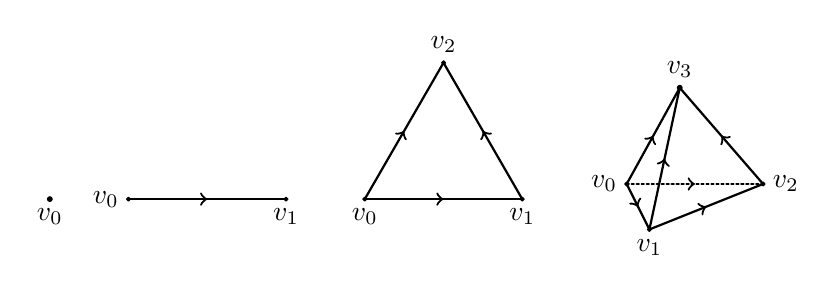
\begin{tikzpicture}[line join = round, line cap = round]

                        % 0-simplex
                        \coordinate [label=below:$v_0$] (0) at (0,0);
                        % 1-simplex
                        \coordinate [label=left:$v_0$] (1) at (1,0);
                        \coordinate [label=below:$v_1$] (2) at (3,0);
                        % 2-simplex
                        \coordinate [label=below:$v_0$] (3) at (4,0);
                        \coordinate [label=below:$v_1$] (4) at (6,0);
                        \coordinate [label=above:$v_2$] (5) at (5,{sqrt(3)});
                        % 3-simpex
                        \coordinate [label=above:$v_3$] (6) at (8,{sqrt(2)},0);
                        \coordinate [label=left:$v_0$] (7) at ({-.5*sqrt(3)+8},0,-.5);
                        \coordinate [label=below:$v_1$] (8) at (8,0,1);
                        \coordinate [label=right:$v_2$] (9) at ({.5*sqrt(3)+8},0,-.5);

                        \begin{scope}[decoration={markings,mark=at position 0.5 with
                            {\arrow{to}}}]
                            % 0-simplex
                            \draw[fill] (0) circle [radius=0.03];
                            % 1-simplex
                            \draw[fill] (1) circle [radius=0.025];
                            \draw[fill] (2) circle [radius=0.025];
                            \draw[thick, postaction={decorate}] (1)--(2);
                            % 2-simplex
                            \draw[fill] (3) circle [radius=0.025];
                            \draw[fill] (4) circle [radius=0.025];
                            \draw[fill] (5) circle [radius=0.025];
                            \draw[thick, postaction={decorate}] (3)--(4);
                            \draw[thick, postaction={decorate}] (3)--(5);
                            \draw[thick, postaction={decorate}] (4)--(5);
                            % 3-simplex
                            \draw[fill] (6) circle [radius=0.03];
                            \draw[fill] (7) circle [radius=0.025];
                            \draw[fill] (8) circle [radius=0.025];
                            \draw[fill] (9) circle [radius=0.025];
                            \draw[thick, densely dotted,postaction={decorate}] (7)--(9);
                            \draw[thick, postaction={decorate}] (7)--(8);
                            \draw[thick, postaction={decorate}] (7)--(6);
                            \draw[thick, postaction={decorate}] (8)--(9);
                            \draw[thick, postaction={decorate}] (8)--(6);
                            \draw[thick, postaction={decorate}] (9)--(6);
                        \end{scope}

                    \end{tikzpicture}
		      
		      
		      
		      The vectors $v_i$, determining  $ [v_0,... , v_n] $
		      are the \emph{vertices} of the simplex.
		      %
		      In our calculations we are going to work with a chosen \emph{ordering} of the vertices of the simplex. I.e., 
		      we are going to use  ``simplex'' when we  mean ``a simplex together with an ordering of the vertices''.
		      %
		      This has a number of consequences. First, it
              determines orientations of the edges $[v_i, v_j]$ according to increasing subscripts.
              Second, specifying an ordering of the vertices  determines
              a canonical linear homeomorphism from   
              $\Delta^n$ onto any $n$-simpex $ [v_0,... , v_n] $ preserving 
              the order of vertices, namely,
              $\sum_i t_i\be_i\mapsto \sum_i t_i \bv_i$.
	      %
	      Once we fix an ordering of the vertices, we also obtain  an orientation of the $n$-simplex, i.e., the sign of
	      $\det(v_0,\ldots,v_n)$. Two orderings determine the same orientation when they differ by an even permutation.
	      
	      By a \emph{face} of a $n$-simplex we shall mean an $(n-1)$-simplex spanned by some $n$-tuple of vertices of the simplex. That is,
	      the $i$-th face of $[v_0,\ldots,v_n]$ is
	       $[v_0,\ldots,\widehat{v_i},\ldots,v_n]$, where the hat indicates omission. Some sources refer to this face as an
	       $(n-1)$-face, and introduce, more generally  \emph{$k$-faces}, for $0\leq k\leq n-1$. These are $k$-simplices, obtained as
	       the convex hull of  a $k$-tuple of vertices. We always order the vertices of a face according to their order
	       in the larger simplex.
	       
	       \begin{Ex}
	       	Consider the (second) face $[v_0,v_1,v_3]$ of the $3$-simplex $[v_0,v_1,v_2,v_3]$ in $\RR^4$. The canonical order-preserving map
	       	$\Delta^2\to [v_0,v_1,v_3]$ is determined by $e_0\mapsto v_0$, $e_1\mapsto v_1$, $e_2\mapsto v_3$. The canonical order-preserving
	       	map from $\Delta^1$ to the edge $[v_1,v_3]$ is determined by $e_0\mapsto v_1$, $e_1\mapsto v_3$.
	       \end{Ex}

	      
		      
		     
                    
             The \emph{boundary} $\partial\Delta^n$ of the standard simplex is defined as the union of all the faces of $\Delta^n$, and
             $\mathring{\Delta}^n = \Delta^n - \partial\Delta^n $ denotes interior of $\Delta^n$. We define analogously the boundary and
             interior of an arbitary simplex in $\RR^n$.
             %
             Notice that with this definition  $\partial \Delta^0=\varnothing$ and $\mathring{\Delta}^0= \Delta^0$!
             
             We now equip $X$ with additional structure: ``parametrization'' of $X$ by simplices of various dimensions that satisfies a number of 
             compatibility conditions.
             
		      \begin{defn}[$\Delta$-complex]\label{Delta-complex}
		      	A $\Delta-complex$ structure on a topological space X is a collection of maps $\left\{\sigma_\alpha: \Delta^n \rightarrow X\right\}_\alpha $,
		      	with $n=n(\alpha)$ depending on the index $\alpha$, such that:
                    \begin{enumerate}
                        \item Each restriction $\sigma_\alpha | \mathring{\Delta}^n$ is                      injective, and each point of X is in the image of exactly one such
                        restriction $\sigma_\alpha | \mathring{\Delta}^n$.
                        \item Each restriction of $\sigma_\alpha$ to a face of $\Delta^n$ is one of the  maps
                        $\sigma_\beta: \Delta^{n-1} \rightarrow X $. Here a face of $\Delta^n$ is identified with $\Delta^{n-1}$ 
                        via the canonical order-preserving linear homeomorphism. 
                        \item A set $A \subset X$ is open iff $\sigma^{-1}_{\alpha}(A)$ is open in $\Delta^n$ for each $\sigma_\alpha$
                    \end{enumerate}

		      \end{defn}
		
		     
		     
		     
		     \begin{Ex}\label{circle_1}
        
        Consider   $ X = S^1 = \{ (x,y) \in \RR^2 \, | \, x^2 + y^2 = 1 \} $. 
        We are going to describe  explicitly two  maps $\sigma_0: \Delta^0 \rightarrow S^1$, $\sigma_1:\Delta^1\to S^1$, which equip
        $S^1$ with the structure of a $\Delta$-complex. 
        
        For the explicit description, keep in mind that $\Delta^0=\{1\}\subseteq \RR$ and that 
         \[ \Delta^1 = \left\{(t_0,t_1)\left| t_0+t_1=1\right.   \right\}  = \{ (t_0, 1-t_0) \, , \, t_0 \in [0, 1] \} \]
         So in particular, any (continuous) map
          $\Delta^1\to S^1$ is determined by and determines  a (continuous) map $[0;1]\to S^1$.
        
	
              
             
              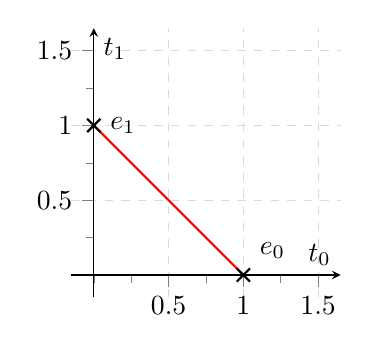
\begin{tikzpicture}
                    \tikzstyle{point}=[thick,draw=black,cross out,inner sep=0pt,minimum width=4pt,minimum height=4pt]
                    \begin{axis}[
                        legend pos=south west,
                        axis x line=middle,
                        axis y line=middle,
                        grid = major,
                        width=5cm,
                        height=5cm,
                        grid style={dashed, gray!30},
                        xmin=0,    % start the diagram at this x-coordinate
                        xmax=1.5,    % end   the diagram at this x-coordinate
                        ymin=0,    % start the diagram at this y-coordinate
                        ymax=1.5,    % end   the diagram at this y-coordinate
                        xlabel=$t_0$,
                        ylabel=$t_1$,
                        tick align=outside,
                        minor tick num=-3,
                        enlargelimits=true,
                        tension=0.08]
                    \addplot[domain=0:1, red, thick,samples=20] {-x+1};
                    \node[point,label={[label distance=0cm]45:$e_0$}] at (axis cs:1,0) {};
                    \node[point,label={[label distance=0cm]0:$e_1$}] at (axis cs:0,1) {};
                    \end{axis}
            \end{tikzpicture}
	      
	      
	            First, we define $\sigma_0: \Delta^0 \rightarrow S^1 $ by  $\sigma_0(1) = (1, 0)$. Next,
		       $\sigma_1: \Delta^1 \rightarrow S^1 $ is defined by  $\sigma_1(t_0,t_1) = (\cos(2\pi t_0), \sin(2\pi t_0))$, 
		       which is clearly continuous.
		       %
		       The map $\sigma_1$ is one-to-one on $\mathring{\Delta}^1$, and so is, trivially, $\sigma_0$ on $\mathring{\Delta}^0$.  The images of the two
		       maps cover the circle, with $\sigma_1\left( \mathring{\Delta}^1\right)=S^1\backslash\{(1,0)\}$ and
		        $\sigma_0\left( \mathring{\Delta}^0\right)=\{(1,0)\}$.
              
              	     
		       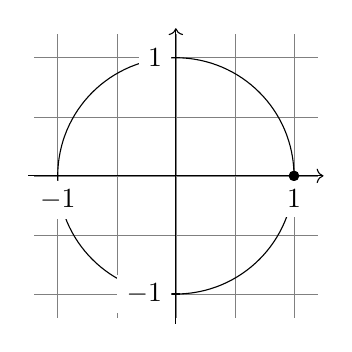
\begin{tikzpicture}[scale=1.5]
                \draw[step=.5cm, gray, very thin] (-1.2,-1.2) grid (1.2,1.2); 
                \draw[->] (-1.25,0) -- (1.25,0) coordinate (x axis);
                \draw[->] (0,-1.25) -- (0,1.25) coordinate (y axis);
                \draw (0,0) circle (1cm);
                \draw[fill] (1,0) circle (0.04);

                \foreach \x/\xtext in {-1, 1} 
                \draw (\x cm,1pt) -- (\x cm,-1pt) node[anchor=north,fill=white] {$\xtext$};
                \foreach \y/\ytext in {-1, 1} 
                \draw (1pt,\y cm) -- (-1pt,\y cm) node[anchor=east,fill=white] {$\ytext$};
                \end{tikzpicture}
              
              
		
              
              
            
              Finally, we check the compatibility property (2) of $\sigma_1$ and $\sigma_0$.
              %
              The restrictions of $\sigma_1$ to the two faces of $\Delta^1$ coincide with $\sigma_0$:
              
              \[
		  \sigma_1|_{[e_1]} = \sigma_1(0,1) = (\cos(0), \sin(0)) = (1, 0)=\sigma_0(1)
              \]
              \[
		  \sigma_1|_{[e_0]} = \sigma_1(1,0) = (\cos(2\pi), \sin(2\pi)) = (1, 0)=\sigma_0(1)
	      \]
              
              Property (3) holds as well.
              There are numerous other $\Delta$-complex structures on $S^1$, and we shall discuss some of them later on.
     \end{Ex}

     \begin{Ex}\label{sphere_1}
        Our next example is a $\Delta$-complex structure on $ X = S^2 = \{ (x,y,z) \in \RR^2 \, | \, x^2 + y^2 + z^2 = 1 \} $.
        
	  Notice first that there is a homeomorphism between the $L^1$-sphere
	  \[
	  	\left\{(x_0,x_1,x_2)\left|\, |x_0|+|x_1|+|x_2|=1 \right. \right\}\subseteq \RR^3
	  \]
	  and $S^2$, given by 
	  \[
	  	(x_0,x_1,x_2)\longmapsto \left(\frac{x_0}{\sqrt{x_0^2+ x_1^2 +x^2_2}}, \frac{x_1}{\sqrt{x^2_0 + x^2_1 + x^2_2}}, \frac{x_2}{\sqrt{x_0^2+ x^2_1 + x^2_2}}, \right),
	  \]
	  that is, by $\bx\longmapsto \frac{\bx}{\|\bx\|}$.
	  
	  On the other hand, the $L^1$-sphere is the union of eight $2$-simplices: one of them is the standard simplex $\Delta^2$ in $\RR^3$, 
	  while the others are obtained from $\Delta^2$ by reflection with respect to a coordinate plane, i.e.,  by multiplying one of the variables by $\pm 1$.
	   Composing with the map between the $L^1$ and $L^2$ sphere, we obtain the
	  eight continuous maps
	  %
	  \[
	  	\sigma_{s_0s_1s_2}:\Delta^2= [e_0, e_1, e_2] \longrightarrow S^2,
	  \]
	  $s_i\in \{\pm 1\}$, $i\in \{0,1,2\}$,
	  \[
	  	\sigma_{s_0s_1s_2}:\ (t_0,t_1,t_2)\longmapsto \left(s_0t_0, s_1t_1, s_2 t_2 \right) \longmapsto \frac{ \left(s_0t_0, s_1t_1, s_2 t_2 \right)  }{\sqrt{t_0^2+t_1^2+t_2^2}}.
	  \]
	  
	  Next, we have the three standard order-preserving homeomorphisms, identifying $\Delta^1$ with the three faces (edges) of
	  $\Delta^1$, $[e_1, e_2]$, $[e_0, e_2]$,  $[e_0, e_1]$. Each of these edges is contained in a coordinate plane in $\RR^3$, 
	  and performing a reflection with respect to the coordinates planes orthogonal to the plane containing the edge gives rise
	  to $12$ maps from $\Delta^1$ to the sphere.
	  
	  Explicitly, these are the 12 continuous maps
	  \[
	  	\lambda_{0s_0s_1}, \lambda_{s_00s_1},\lambda_{s_0s_10}: \Delta^1 \longrightarrow S^2,\ 
	  \]
	  where $s_i\in \{\pm 1\}$ and
	  \[
	  	\lambda_{0s_0s_1}: (t_0,t_1)\longmapsto (0,s_0t_0,s_1t_1)\longmapsto \frac{(0,s_0t_0,s_1t_1)}{\sqrt{t_0^2+t_1^2}}
	  \]
	  \[
	  	\lambda_{s_00s_1}: (t_0,t_1)\longmapsto (s_0t_0,0,s_1t_1)\longmapsto \frac{(s_0t_0,0,s_1t_1)}{\sqrt{t_0^2+t_1^2}}
	  \]
	  \[
	  	\lambda_{s_0s_10}: (t_0,t_1)\longmapsto (s_0t_0,s_1t_1,0)\longmapsto \frac{(s_0t_0,s_1t_1,0)}{\sqrt{t_0^2+t_1^2}}.
	  \]
	  
	  Finally, we have six maps $\Delta^0\to S^2$, obtained by composing the three inclusions of $\Delta^0$ as a $0$-face in $\Delta^2$, c
	  composed with reflections with respect to the coordinate planes. Explicitly, these are the 6 maps
	  \[
	  	\mu_{s00}, \mu_{0s0},\mu_{00s}: \Delta^1 \longrightarrow S^2,
	  \]
	  where $s\in \{\pm 1\}$ and
	  \[
	  	\mu_{s00}(1)=(s,0,0), \ \mu_{0s0}(1)=(0,s,0),\ \mu_{00s}(1)= (0,0,s).
	  \]
	  
	  The images of the maps cover $S^2$, they are injective when restricted to the interiors of the simplices
	  and are compatible. For example, $ \sigma_{s_0s_1s_2}\left|_{[e_1,e_2]}\right. = \lambda_{0s_1s_2}$, 
	  $\lambda_{s_0s_10}|_{[e_0]}=\mu_{s_000}$, etc. suppressing the canonical orientation-preserving 
	  homeomorphism between simplices.
	  %
	  Moreover, property (3) is satisfied. We do not check it explicitly, but it follows from the fact that
	  our maps are obtained as composition of inclusion of a face into a simplex, followed by a reflection and 
	  a homeomorphism between the $L^1$ and $L^2$ sphere.
	  
	  Altogether, this $\Delta$-complex structure on $S^2$ consists of the eight maps $\sigma_{s_0s_1s_2}$, 
	  the twelve maps $\lambda_{0s_0s_1}, \lambda_{s_00s_1},\lambda_{s_0s_10}$ and the six maps
	  $\mu_{s00}, \mu_{0s0},\mu_{00s}$.








		     
		      
              
              
            \tdplotsetmaincoords{70}{130}
            \begin{tikzpicture}[tdplot_main_coords, scale=2]
                    \def\laxis{2}
                    \def\ltriangle{1}
                    \def\ltick{.2}
                    %%% axes
                    \draw [->] (0,0,0) -- (\laxis,0,0) node [below] {$t_0$};
                    \draw [->] (0,0,0) -- (0,\laxis,0) node [right] {$t_1$};
                    \draw [->] (0,0,0) -- (0,0,\laxis) node [left] {$t_2$};
                    
                    \draw [->, ultra thick] (0,0,0) -- (\ltriangle,0,0) node [below] {$e_0$};
                    \draw [->, ultra thick] (0,0,0) -- (0,\ltriangle,0) node [right] {$e_1$};
                    \draw [->, ultra thick] (0,0,0) -- (0,0,\ltriangle) node [left] {$e_2$};
                    %%% axes ticks
                    \pgfmathtruncatemacro{\nticks}{floor(\laxis)-1}
                    \begin{scope}[
                        help lines,
                        every node/.style={inner sep=1pt,text=black}
                        ]
                        \foreach \coord in {1,...,\nticks} {
                        \draw (\coord,\ltick,0) -- ++(0,-\ltick,0) -- ++(0,0,\ltick)
                        node [pos=1,left] {\coord};
                        \draw (\ltick,\coord,0) -- ++(-\ltick,0,0) -- ++(0,0,\ltick)
                        node [pos=1,right] {\coord};
                        \draw (\ltick,0,\coord) -- ++(-\ltick,0,0) -- ++(0,\ltick,0)
                        node [at start,above right] {\coord};
                        }
                    \end{scope}
                    %%% figure
                    \filldraw [opacity=.33,red] (\ltriangle,0,0) -- (0,\ltriangle,0)
                    -- (0,0,\ltriangle) -- cycle;
            \end{tikzpicture}
              

     \end{Ex}
     
	  For completeness, we mention  some ``non-examples'': collections of maps $\sigma_\alpha:\Delta^n\to X$ that satisfy conditions (1) and (2), but not condition (3) from Definiton \ref{Delta-complex}.
     \begin{Ex}
     	Let $X=[0;1]$ or more generally, any other non-discrete space, having infinitely many points. Then the collection
     	of  maps $\{\sigma_x:\Delta^0\to X\}_{x\in X}$, $\sigma_x(1)=x$ 
     	satisfies (1) and (2), but not (3). We place  one $0$-simplex for each point of $X$, but  points in $[0;1]$ are not open.
     	
     	Another  example is as follows. Let $X$ be the unit square $X=[0;1]\times [0;1]$. Consider, for each $y\in [0;1]$, a  map
     	$\lambda_y:\Delta^0\to X$, $\lambda_y(1)=(0,y)$, a map $\rho_y:\Delta^0\to X$, $\rho_y(1)=(1,y)$ and a map
     	$\sigma_y:\Delta^1\to X$, $\sigma_y(t_0,t_1)= (t_0,y)$. In this way we place  at height $y$ one $1$-simplex (as a horizontal segment), 
     	and two $0$-simplices, as its left and right end. The collection of maps $\{\sigma_y, \lambda_y, \rho_y\}_{y\in[0;1]}$ satisfies (1) and (2), 
     	but not (3).
     \end{Ex}
	  Thus condition (3) precludes inadequate choices of maps $\sigma_\alpha$, for example, covering a manifold (with boundary) of dimension $n$ by simplices
	  of smaller dimension.
	  More generally, condition (3) is important when one needs to deal with  infinite collections of simplices, in particular, when dealing with
	  infinite-dimensional (in appropriate sense) spaces $X$.
	  
	  
	  
	  Given a $\Delta$-complex structure on $X$, we can recover the space just from the combinatorics of the maps $\left\{\sigma_\alpha:\Delta^{n(\alpha)}\to X\right\}_{\alpha\in A}$.
	  More precisely, we can consider the disjoint union of  simplices $\Delta_\alpha^n$, labelled by the respective maps $\sigma_\alpha$. We then impose an
	  equivalence relation $\sim$ on the disjoint union: the $i$-th face of $\Delta^n_\alpha$ is identified with $\Delta^{n-1}_\beta$ 
	  via the canonical order-preserving isomorphism
	  if $\left. \sigma_\alpha\right|_{[e_0,\ldots, \widehat{e_i},\ldots e_n]}$
	  coincides with $\sigma_\beta:\Delta^{n-1}\to X$ (under the canonical isomorphism).
	  
	  The properties (1), (2), (3) from Definition \ref{Delta-complex} guarantee that the quotient space is indeed homeomorphic to $X$:
	  
	  \[
	  	X \simeq \left. \coprod_{\alpha\in A}\Delta^{n}_\alpha\right/ \sim.
	  \]
	  
	  Turning this viewpoint backwords, we can consider $X$ as being built up, inductively, by simplices of dimension $0$, $1$, $2$, \ldots, 
	  by imposing an equivalence relation, encoded combinatorially.
	  
	  \begin{Ex}
	  	Consider the $\Delta$-complex structure on $S^1$, discussed in Example \ref{circle_1}. It gives an identification
	  	of $S^1$ as a quotient of $\Delta^0\sqcup \Delta^1$, i.e., 
	  	\[
	  		S^1\simeq \left. \Delta_0^0\coprod \Delta^1_1\right/\sim,
	  	\]
	  	where the equivalence relation identifies the point $\Delta_0^0$ with each of the endpoints of the $1$-simplex $\Delta_1^1$.
	  	
	  	Similarly, the $\Delta$-complex structure on $S^2$ from Example  \ref{sphere_1} identifies $S^2$ with a quotient of
	  	\[
	  		\underbrace{\Delta^0\sqcup \ldots \sqcup \Delta^0}_{6}\coprod \underbrace{\Delta^1\sqcup \ldots \sqcup\Delta^1}_{12}\coprod \underbrace{\Delta^2\sqcup \ldots \sqcup\Delta^2}_{8}.
	  	\]
	  	The equivalence relation is encoded in the maps, and can be made explicit by labelling each simplex with the respective map, 
	  	e.g., $\Delta^0_{\mu_{s00}}$, $\Delta^0_{\mu_{0s0}}$, $\Delta^0_{\mu_{00s}}$, $\Delta^1_{\lambda_{0s_0s_1}}$,\ldots, $\Delta^2_{\sigma_{s_0s_1s_2}}$.


	  \end{Ex}
	  
	  One often constructs topological spaces as quotients, i.e., we write $X=Y/\sim$, where $Y$ is a possibly simpler space. This is the case, for instance, for
	  $X=S^1\times S^1$, $X=\RR\PP^2$, the Klein bottle, etc. In all of these examples $Y=[0;1]\times [0;1]$. One can try to build a $\Delta$-complex structure
	  on $X$ by constructing first a $\Delta$-complex structure on $Y$. We are going to see such examples in Section \ref{homology_ex}.
	  
	  \subsection*{A Remark on Simplicial Complexes}
	  
	  The $\Delta$-complex structure on $S^1$ from Example \ref{circle_1} involves one $1$-simplex and one $0$-simplex, and the gluing identifies the two vertices of
	  $\Delta^1$. We could, however, choose different $\Delta$-structures, e.g., one involving two (or more) $1$-simplices -- see Section \ref{homology_ex}.
	  In that case each $1$-simplex in $X$ will have two distinct vertices -- i.e., the maps $\sigma_\alpha:\Delta^1\to S^1$ do not identify the vertices
	  of $\Delta^1$. (Equivalently, the equivalence relation $\sim$ does not identify distinct vertices.)
	  
	  More generally, we say that a $\Delta$-complex (structure on a topological space) $X$ is a \emph{simplicial complex} (structure on $X$) if all  simplices are
	  uniquely determined by their vertices. That is, for all $n\in \NN$ it is the case that each $n$-simplex in $X$ has $n+1$ 
	  distinct vertices and there are no other $n$-simplices with this set of vertices. 
	  %
	  %
	  Now, in such a situation, every face of an $n$-simplex in $X$ is an $(n-1)$-simplex in $X$, and so on. 
	  
	  But 
	  such a structure is  a  completely combinatorial object! It is specified by a finite set -- the $0$-complexes of our $\Delta$-structure,
	  together with finite subsets (corresponding to simplices in $X$), having the property that all of their subsets are also simplices.
	  
	  
	  
	  
	   Here is the formal combinatorial description of a simplicial complex, given as the definition of an \emph{abstract simplicial complex}. 


		     
		     
		     \begin{defn} [Abstract  Simplicial Complex] 
              Given a finite  set $  \{1, 2, \cdots, m\} (=[m])$ 
              an \emph{ abstract simplicial complex} is a collection $\mathcal{K}$ of subsets of $[m]$,  such that:
              \begin{enumerate}
              \item $\emptyset \in \mathcal{K}$
              \item $\{i\} \in \mathcal{K}$ (singletons are in $\cK$)
              \item If $ I \in \mathcal{K} $ and $J\subseteq I$, then $\mathcal{J} \in \mathcal{K}$
              \end{enumerate}
              The elements of $[m]$ are the \emph{vertices}, and the elements of $\cK$ are the \emph{simplices}, where $I\in \cK$ is
              an $(|I|-1)$-simplex.
		     \end{defn}
		     Sometimes, the condition $\varnothing\in \cK$ is omitted. Abstract simplices are subsets of the power set of the given set of vertices, 
		     which are partially ordered by inclusion.

            
%               $(\forall I \in \mathcal{K} (\forall J \subseteq I)) \Rightarrow \mathcal{J} \in \mathcal{K}$\\
            \begin{Ex}
              Consider the following partially ordereed set  $ V = \{1, 2, 3, 4\}$: 
              The simplicial complex 
              $\mathcal{K} = \{I = \{1, 2, 3\}, \{1, 2\}, \{1, 3\}, \{2, 3\}, \{1\}, \{2\}, \{3\}, \{4\}, \emptyset\}$
             
             \begin{center}
              

              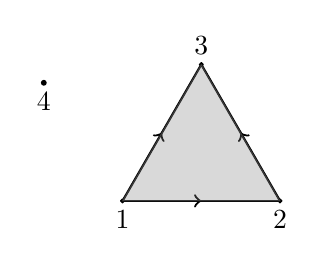
\begin{tikzpicture}[line join = round, line cap = round]

                % 0-simplex
                \coordinate [label=below:$4$] (0) at (3,1.5);
                % 2-simplex
                \coordinate [label=below:$1$] (1) at (4,0);
                \coordinate [label=below:$2$] (2) at (6,0);
                \coordinate [label=above:$3$] (3) at (5,{sqrt(3)});

                \begin{scope}[decoration={markings,mark=at position 0.5 with
                    {\arrow{to}}}]
                  % 0-simplex
                  \draw[fill] (0) circle [radius=0.03];
                  % 2-simplex
                  \draw[fill] (1) circle [radius=0.025];
                  \draw[fill] (2) circle [radius=0.025];
                  \draw[fill] (3) circle [radius=0.025];
                  \draw[thick, postaction={decorate}] (1)--(2);
                  \draw[thick, postaction={decorate}] (1)--(3);
                  \draw[thick, postaction={decorate}] (2)--(3);
                  \filldraw[opacity=.3, gray] (1) --  (2) --  (3) -- cycle;

                \end{scope}
              \end{tikzpicture}
             
             \end{center}
             
             Given an abstract simplex $\cK$, we can construct its
             \emph{topological realization}  as
             
              \[|\mathcal{K}| = \underset{\varnothing \neq I\in \cK }{\bigcup} (\textrm{Conv}(e_i),i\in I)\subseteq \RR^m\] 
              where $\{e_i\}$ is in the standard basis $e_1, \cdots e_m \in \mathbb{R}^m$. 
            \end{Ex}
            
            
            Classically, homology theories were introduced for simplicial complexes (while $\Delta$-complexes were also called semi-simplicial complexes).
            Simplicial complexes have simple combinatorial description and are widely used in computer implementations of homology calculations. For the purposes of human 
            understanding, however, $\Delta$-complexes are much more convenient.
            
            A subcomplex of $\mathcal{K}$ is a subset $L \subseteq \mathcal{K}$ that is also a simplicial complex.
            \label{complexfiltration}
            A \emph{filtration} of complex $\mathcal{K}$ is a nested subsequence of complexes: 
             \[
              \emptyset = \mathcal{K}^0 \subseteq \mathcal{K}^1 \subseteq \dots \mathcal{K}^m = \mathcal{K}  
             \]
             For generality, we let $\mathcal{K}^i = \mathcal{K}^m$ for all $i \geq m$. $\mathcal{K}$ is called a filetered complex, and below there is a short example of a filtered complex: 
             
             \begin{center}
              
            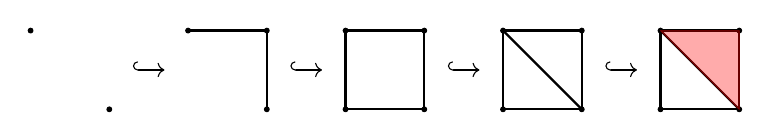
\begin{tikzpicture}[line join = round, line cap = round]
                % 1st
                \coordinate (0) at (0,1);
                \coordinate (1) at (1,0);
                % arrow 1st to 2nd
                \coordinate (a1) at (1.3, 0.5);
                \coordinate (a2) at (1.7, 0.5);
                % 2nd
                \coordinate (2) at (2,1);
                \coordinate (3) at (3,0);
                \coordinate (4) at (3,1);
                % arrow 2nd to 3rd
                \coordinate (a3) at (3.3, 0.5);
                \coordinate (a4) at (3.7, 0.5);
                % 3rd
                \coordinate (5) at (4,1);
                \coordinate (6) at (4,0);
                \coordinate (7) at (5,1);
                \coordinate (8) at (5,0);
                % arrow 3rd to 4th
                \coordinate (a5) at (5.3, 0.5);
                \coordinate (a6) at (5.7, 0.5);
                % 4th
                \coordinate (9) at (6,1);
                \coordinate (10) at (6,0);
                \coordinate (11) at (7,1);
                \coordinate (12) at (7,0);
                % arrow 4th to 5th
                \coordinate (a7) at (7.3, 0.5);
                \coordinate (a8) at (7.7, 0.5);
                % 5th
                \coordinate (13) at (8,1);
                \coordinate (14) at (8,0);
                \coordinate (15) at (9,1);
                \coordinate (16) at (9,0);

                \begin{scope}[decoration={markings,mark=at position 0.5 with {\arrow{to}}}]
                  \draw[fill] (0) circle [radius=0.03];
                  \draw[fill] (1) circle [radius=0.03];
                  \draw[fill] (2) circle [radius=0.03];
                  \draw[fill] (3) circle [radius=0.03];
                  \draw[fill] (4) circle [radius=0.03];
                  \draw[fill] (5) circle [radius=0.03];
                  \draw[fill] (6) circle [radius=0.03];
                  \draw[fill] (7) circle [radius=0.03];
                  \draw[fill] (8) circle [radius=0.03];
                  \draw[fill] (9) circle [radius=0.03];
                  \draw[fill] (10) circle [radius=0.03];
                  \draw[fill] (11) circle [radius=0.03];
                  \draw[fill] (12) circle [radius=0.03];
                  \draw[fill] (13) circle [radius=0.03];
                  \draw[fill] (14) circle [radius=0.03];
                  \draw[fill] (15) circle [radius=0.03];
                  \draw[fill] (16) circle [radius=0.03];
                  % hooks
                  \draw [right hook->] (a1) -- (a2);
                  \draw [right hook->] (a3) -- (a4);
                  \draw [right hook->] (a5) -- (a6);
                  \draw [right hook->] (a7) -- (a8);
                  % 2nd
                  \draw[thick] (3)--(4);
                  \draw[thick] (2)--(4);
                  % 3rd
                  \draw[thick] (5)--(6);
                  \draw[thick] (5)--(7);
                  \draw[thick] (6)--(8);
                  \draw[thick] (7)--(8);
                  % 4th
                  \draw[thick] (9)--(10);
                  \draw[thick] (9)--(11);
                  \draw[thick] (10)--(12);
                  \draw[thick] (11)--(12);
                  \draw[thick] (9)--(12);
                  % 5th
                  \draw[thick] (13)--(14);
                  \draw[thick] (13)--(15);
                  \draw[thick] (14)--(16);
                  \draw[thick] (15)--(16);
                  \draw[thick] (13)--(16);
                \end{scope}
                \filldraw [opacity=.33,red] (8,1) -- (9,1) -- (9,0) -- cycle;
              \end{tikzpicture}
             \end{center}

		      

		\section{Chain Complexes and Homology}

        One of the key algebraic notions that we need is the notion of \emph{chain complex}.
		
             \begin{defn}[Chain complex]
		      	   Complex of abelian groups. Homology of a complex.\\
		      	   A \emph{chain complex} $(C_\bullet,\partial_\bullet)$ is a sequence of homomorphisms of abelian groups:
		      	   \[
                        \xymatrix{
                            {...}  \ar[r] &
                            C_{n+1}  \ar[r]^{\partial_{n+1}} &
                            C_n  \ar[r]^{\partial_n} &
                            C_{n-1}  \ar[r]^{\partial_{n-1}} &
                            {...}  \ar[r] &
                            C_1  \ar[r]^{\partial_1} &
                            C_0  \ar[r]^{\partial_0 = 0}
                            & 0 \\ }
                   \]
		      	   where \(\partial_n\partial_{n+1}=0\) for each $n\in \NN$. The equation
		      	   \(\partial_n\partial_{n+1}=0\) is equivalent to the inclusion $ \Ima\partial_{n+1} \subset \ker\partial_n $. The elements of $\ker \partial _n$ are called \emph{$n$-cycles}, often denoted $Z_n$. The elements of $\Ima\partial_{n+1}\subseteq C_n$ are called \emph{$n$-boundaries}, often denoted $B_n$. The \emph{$n$-th homology group} of the complex is the quotient $H_n(C_\bullet)=\ker \partial_n/\Ima\partial_{n+1}$. The  maps $\partial_n$ are called \emph{the differentials} or \emph{the boundary maps} of the complex.
		      \end{defn}

		      One often considers a collection of groups $C_n$ labelled by $n\in \ZZ$ -- and in any case can extend from $n\in \NN$ to $n\in \ZZ$ by setting $C_n=(0)$ for $n<0$. The chain groups ($n$-chains) are often thought of as a single object, a \emph{graded group} $C_\bullet=\bigoplus_n C_n$. We denoted by $C_\bullet[k]$ the graded group, whose grading is shifted by $k$, i.e., $(C_\bullet[k])_n= C_{n+k}$. The differentials $\partial_n$ can be thought of as a map of graded groups $\partial: C_\bullet\to C_\bullet[-1]$, satisfying the condition $\partial^2=0$.
		      
		       In algebraic topology, we construct various complexes of abelian groups, associated with a space $X$ and study  their homology groups.
		       
		       We start with a space $X$, equipped with a $\Delta$-complex structure. We associate with it a collection of groups $C_n:=\Delta_n(X)$, $n\geq 0$ -- the simplicial $n$-chains -- as follows. The group $\Delta_n(X)$ is the free abelian group, generated by the (images of the) open simplices $e_\alpha^n:= \sigma_\alpha(\mathring{\Delta}^n)$.  Thus its elements are linear combinations with integer coefficients, $\sum_\alpha n_\alpha e_\alpha^n$. Equivalently, and more conveniently, we think of $\Delta_n(X)$ as the free group on the maps $\sigma_\alpha:\Delta^n\to X$.
		      
		      The boundary map
		      $\partial_n: \Delta_n(\mathcal{X}) \rightarrow \Delta_{n-1}(\mathcal{X})$ for the would-be chain complex $\Delta_\bullet(X)$ is defined as
		      \[
		         \partial_n(\sigma_\alpha) = \sum\limits_i (-1)^i \sigma_\alpha | [v_0, ... ,\widehat{v_i}, ... , v_n].
              \]

            \begin{Lemma}\label{delta2}
             The composition $\partial^2=0$ below is zero
             \[
                \xymatrix{
                    \Delta_n(X)  \ar[r]^{\partial_n} &
                    \Delta_{n-1}(X)  \ar[r]^{\partial_{n-1}} &
                    \Delta_{n-2}(X)   \\ }.
             \]
             That is, $(\Delta_\bullet(X),\partial_\bullet)$ is a chain complex.
            \end{Lemma}

            \emph{Proof}: As a preliminary illustration, let us prove that $\partial_2 \partial_3 = 0$:
             \[
                \xymatrix{
                    \Delta_3(X)  \ar[r]^{\partial_3} &
                    \Delta_2(X)  \ar[r]^{\partial_2} &
                    \Delta_1(X)   \\ }
             \]
             We have, for $\sigma\in \Delta_3(X)$, \[\partial_3\sigma = \sum\limits_i (-1)^i \sigma | [v_0, ... ,\widehat{v_i}, v_3] =
             \sigma | [v_1, v_2, v_3] - \sigma | [v_0, v_2, v_3] + \sigma | [v_0, v_1, v_3] - \sigma | [v_0, v_1, v_2]\]


            \begin{equation}
                \begin{aligned}
                    \partial_2 \partial_3(\sigma) &= \sigma | [v_2, v_3] - \sigma | [v_1, v_3] + \sigma | [v_1, v_2] \\
                    &= -\sigma | [v_2, v_3] + \sigma | [v_0, v_3] - \sigma | [v_0, v_2] \\
                    &= \sigma | [v_1, v_3] - \sigma | [v_0, v_3] + \sigma | [v_0, v_1] \\
                    &= -\sigma | [v_1, v_2] + \sigma | [v_0, v_2] - \sigma | [v_0, v_1] = 0
                \end{aligned}
            \end{equation}

        In case of arbitary  $n$ the proof proceeds analogously.

            \begin{equation}
                \begin{aligned}
                    \partial_{n-1} \partial_n(\sigma) &=  \partial_{n-1}(\sum\limits_i (-1)^i \sigma | [v_0, ... ,\hat{v_i}, ... , v_n]) \\
                    &=  \sum\limits_j (-1)^j ( \sum\limits_i (-1)^i \sigma | [v_0, ... ,\hat{v_i}, ... , v_n]) | [v_0, ... ,\hat{v_j}, ... , v_n] \\
                    &=  \sum\limits_{j<i} (-1)^i(-1)^j  \sigma_ | [v_0, ... ,\hat{v_j},... ,\hat{v_i} ... , v_n] +
                    \sum\limits_{j>i} (-1)^i(-1)^{j}  \sigma_ | [v_0, ... ,\hat{v_i},... ,\hat{v_j} ... , v_n] = 0
                \end{aligned}
            \end{equation}
            
            \qed
            
            The homology groups of the complex $(\Delta_\bullet(X), \partial_\bullet)$ are called \emph{the simplicial homology groups of $X$} and denoted by $H^\Delta_n(X)$, $n\geq 0$.

        The superscript $\Delta$ in $H^\Delta_n(X)$ indicates that, properly speaking, these groups are defined for a $\Delta$-complex $X$, i.e., for a topological space $X$ with some additional structure. In fact, it is a very important result that these groups \emph{do not} depend on the chosen $\Delta$-complex structure. We are going to discuss this more in the next chapter. See also the comparison theorem for simplicial and singular homology in \cite{hatcher}[2.1]. In view of this, we may occasionally drop the superscript $\Delta$ and write $H_n(X)$ for the $n$-th simplicial homology of $X$.
            
        \emph{Remark: } Chain complexes can be also defined over $R-modules$, where $R$ is a commutative ring:

        \begin{defn} (Chain complex of $R$-module)
        A Chain complex of $R$-modules is a sequence:
                \[ (C_\bullet, d_\bullet)= (
                        \xymatrix{
                            {...}  \ar[r] &
                            C_{n+1}  \ar[r]^{d_{n+1}} &
                            C_n  \ar[r]^{d_n} &
                            C_{n-1}  \ar[r]^{d_{n-1}} &
                            {...}
                             } )
                   \]
        where for each $n \in \ZZ$, $C_n$ is an $R$-module and $d_n \in Hom_{R}(C_n, C_{n-1})$ satisfies
        $d_n \circ d_{n+1} = 0$.
        \end{defn}

        %In chain complexes of $R-modules$, n is the degree of the $R-module \ C_n$. The $R-linear$ maps
        %$d_n (n \in \ZZ)$ are called differential maps. \\
        %Also, a complex $C_\bullet$ is called non-negative (resp. positive) if $C_n = 0$, for all $n \in \ZZ_{<0}$ (resp. $n \in \ZZ_{\leq 0}$)

        Chain complexes together with morphisms of chain complexes (and composition given by
        degreewise composition of $R$-morphisms) form a category, which we will denote by $Ch(_RMod)$

		 \section{Homology Calculations: Examples}\label{homology_ex}

		 \subsection{Homology of the circle $ S^1$}
		 We begin with computing the simplicial homology groups of the circle $S^1$. We will do so with respect to two different
                $\Delta$-complex structures and will observe that, while the complexes $\Delta_n(S^1)$ will be different, their homology will be isomorphic.
                
                \subsubsection{Method I: Triangulation}
                To compute the homolgy group of the circle $S^1$ we can triangulate the circle in the following way: \\

                \[
                       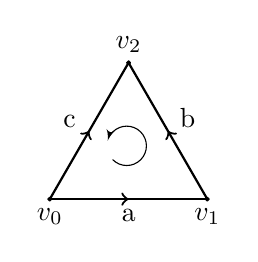
\begin{tikzpicture}[line join = round, line cap = round]

                                % 2-simplex
                                \coordinate [label=below:$v_0$] (3) at (4,0);
                                \coordinate [label=below:$v_1$] (4) at (6,0);
                                \coordinate [label=above:$v_2$] (5) at (5,{sqrt(3)});
                                \coordinate (0) at (4.8, 0.5);


                                \begin{scope}[decoration={markings,mark=at position 0.5 with {\arrow{to}}}]


                                    \draw[fill] (3) circle [radius=0.025];
                                    \draw[fill] (4) circle [radius=0.025];
                                    \draw[fill] (5) circle [radius=0.025];
                                    \draw[thick, postaction={decorate}] (3)--(4) node [midway, below] {a};
                                    \draw[thick, postaction={decorate}] (3)--(5) node [near start, above=10pt] {c};

                                    \draw[thick, postaction={decorate}] (4)--(5) node [near start, above=10pt] {b};
                                    \draw[->,>=latex'] (0) arc[radius=0.25,start angle=225,delta angle=300];

                                \end{scope}
                    \end{tikzpicture}
                    \]
                    We can construct the following chain complex which is a sequence of homomorphisms of abelian groups:

	\[
		\xymatrix{
			0  \ar[r]^{\partial_2 = 0} &
			C_1  \ar[r]^{\partial_1} &
			C_0  \ar[r]^{\partial_0 = 0}
			& 0 \\ }
	\]

 where \(\partial_n\partial_{n+1}=0\) for each n  in $\mathbb{Z}$ and

			\[
				\left|
				  \begin{array}{l}
				  	C_0= \langle v_0, v_1, v_2 \rangle \\
				  	C_1=\langle a, b, c \rangle \\
                    C_n=\{0\} \quad \forall n \geqslant 2
				  \end{array}
				\right.,
			\]

			\[
                \xymatrix{
                    0  \ar[r]^{\partial_2 = 0} &
                    \mathbb{Z}^{\oplus^3}  \ar[r]^{\partial_1} &
                    \mathbb{Z}^{\oplus^3}  \ar[r]^{\partial_0 = 0}
                    & 0 \\ }
	        \]
The n-th homology group is defined as $H_n = \frac{\ker\partial_n}{\Ima\partial_{n+1}}$. \\

\par
First, let's compute $H_0$: \\
$\ker\partial_0 = C_0 = \langle v_0, v_1, v_2 \rangle$ since $\partial_0 = 0$ \\
To calculate $\Ima\partial_1$, let's compute $\partial_1(\alpha a + \beta b + \gamma c) = \alpha (v_1-v_0) + \beta (v_2-v_1) - \gamma (v_2-v_0) \\ = (-\alpha + \gamma)v_0 + (\alpha - \beta)v_1 + (\beta - \gamma)v_2 = (\gamma -\alpha)v_0 + (\alpha - \beta)v_1 + (-(\gamma - \alpha)-(\alpha - \beta))v_2 $ \\
$\Ima\partial_1 = \left\{ \left(\begin{array}{c}
          		                 	( \gamma - \alpha )\\
          		                 	(\alpha - \beta)\\
          		                 	-(\gamma - \alpha)-(\alpha - \beta)\\
          		                 \end{array} \right), \quad \alpha, \beta, \gamma \subseteq \mathbb{Z} \right\} \subseteq \mathbb{Z}^{\oplus^3} $ \\

$Claim: $ There exist an isomorphism $\psi: \Ima\partial_1 \simeq \mathbb{Z}^2$\\
$\psi: \left(\begin{array}{c}
                    ( \gamma - \alpha )\\
                    (\alpha - \beta)\\
                    (\beta - \gamma)\\
            \end{array} \right) \mapsto
            \left(\begin{array}{c}
                    ( \gamma - \alpha )\\
                    (\alpha - \beta)\\
            \end{array} \right)$ \\
$\psi $ is one-to-one since if $ ( \gamma - \alpha  = 0 \; \& \; \alpha - \beta = 0) \Rightarrow \beta - \gamma = 0  \; \& \; \alpha = \beta = \gamma $ \\
$\psi $ is onto since given $\left(\begin{array}{c}
                    m\\
                    n\\
            \end{array} \right) \in \mathbb{Z}^2$
        there exist an element $\left(\begin{array}{c}
                    m\\
                    n\\
                    -m-n\\
            \end{array} \right) \in \Ima\partial_1 $ such that \\
$\psi \left(\begin{array}{c}
                    m\\
                    n\\
                    -m-n\\
            \end{array} \right) =
      \left(\begin{array}{c}
                    m\\
                    n\\
            \end{array} \right)$, since $\psi$ is one-to-one and onto, $\Ima\partial_1 \simeq \mathbb{Z}^2$

$H_0 = \frac{\ker\partial_0}{\Ima\partial_1} = \mathbb{Z}^{3} \left/ {
    \left(\begin{array}{c}
                    1\\
                    0\\
                    -1\\
            \end{array} \right)\mathbb{Z} \oplus
    \left(\begin{array}{c}
                    0\\
                    1\\
                    -1\\
            \end{array} \right)\mathbb{Z}} \right.$ \\

    Claim: $ \phi: \left( \mathbb{Z}^{3} \left/ {
    \left(\begin{array}{c}
                    1\\
                    0\\
                    -1\\
            \end{array} \right)\mathbb{Z} \oplus
    \left(\begin{array}{c}
                    0\\
                    1\\
                    -1\\
            \end{array} \right)\mathbb{Z}} \right. \right) \simeq \mathbb{Z}$ \\

            First, let us take the map $\varphi: \mathbb{Z}^{3} \rightarrow \mathbb{Z}^{3} \left/
            \left\langle \left( \begin{array}{c}
                    1\\
                    0\\
                    -1\\
            \end{array} \right), \left(\begin{array}{c}
                    0\\
                    1\\
                    -1\\
            \end{array} \right)  \right\rangle \right.$ \\
$\mathbb{Z}^{3} \ni  \left(\begin{array}{c}
                    p\\
                    q\\
                    r\\
            \end{array} \right) =
            p\left(\begin{array}{c}
                    1\\
                    0\\
                    -1\\
            \end{array} \right) +
            q\left(\begin{array}{c}
                    0\\
                    1\\
                    -1\\
            \end{array} \right) +
            (p+q+r)\left(\begin{array}{c}
                    0\\
                    0\\
                    1\\
            \end{array} \right) $ \\ where $
            p\left(\begin{array}{c}
                    1\\
                    0\\
                    -1\\
            \end{array} \right) +
            q\left(\begin{array}{c}
                    0\\
                    1\\
                    -1\\
            \end{array} \right) \in \left(\begin{array}{c}
                    1\\
                    0\\
                    -1\\
            \end{array} \right)\mathbb{Z} +
    \left(\begin{array}{c}
                    0\\
                    1\\
                    -1\\
            \end{array} \right)\mathbb{Z} $ \\

So, $\varphi: \left(\begin{array}{c}
                    p\\
                    q\\
                    r\\
            \end{array} \right) \mapsto \overline{\left(\begin{array}{c}
                    p\\
                    q\\
                    r\\
            \end{array} \right)} = (p+q+r) \overline{\left(\begin{array}{c}
                    0\\
                    0\\
                    1\\
            \end{array} \right)}$ \\

           Finally, $ \phi: \overline{\left(\begin{array}{c}
                    p\\
                    q\\
                    r\\
            \end{array} \right)} \mapsto (p+q+r) \in \mathbb{Z} $, Clearly, $\phi$ is injective and surjective.

          So, $H_0 \simeq \mathbb{Z} $ \\

\par
Second, let's compute $H_1$: \\
$\ker\partial_1 = \left\{ \left(\begin{array}{c}
                    m\\
                    m\\
                    m\\
            \end{array} \right), m \in \mathbb{Z} = \right\} = \left(\begin{array}{c}
                    1\\
                    1\\
                    1\\
            \end{array} \right) \mathbb{Z} \simeq \mathbb{Z}$ \\
$\Ima\partial_2 = \{0\}$ since $C_2 = \{0\}$ \\
$H_1 = \frac{\ker\partial_1}{\Ima\partial_2} =
		\frac{ \ker{\partial_1} }{ \{0\} } = \ker{\partial_1} \simeq \mathbb{Z}$ \\


Finally, the homology groups of the circle are:
		\[
	  		H_n^\Delta(S^1) \simeq \left\{
			      \begin{array}{rl}
			     \mathbb{Z}, & \textrm{for} \: n = 0, 1\\

                        0 & \textrm{for} \: n \geqslant 2
			      \end{array}
			 \right.
	  	\]

 \subsubsection{Method II}
                  To compute the homolgy group of the circle $S^1$ we can construct the circle, by two vertices and two edges, in the following way: \\

              \[
              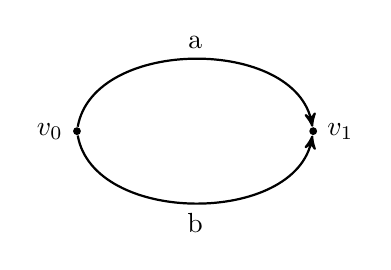
\begin{tikzpicture}[>=stealth',x=1cm, y=1cm]

                  \draw (0,0) node[circle, inner sep=1pt, fill=black, label={left:{$v_0$}}] (A) {};
                  \draw (3,0) node[circle, inner sep=1pt, fill=black, label={right:{$v_1$}}] (B) {};
                  \draw [thick, ->] (A) to [out=80, in=100] node[midway, above]{a} (B) ;
                  \draw [thick, ->] (A) to [out=280, in=260] node[midway, below]{b} (B) ;

                \end{tikzpicture}
                \]
                    We can construct the following chain complex which is a sequence of homomorphisms of abelian groups:

	\[
		\xymatrix{
			0  \ar[r]^{\partial_2 = 0} &
			C_1  \ar[r]^{\partial_1} &
			C_0  \ar[r]^{\partial_0 = 0}
			& 0 \\ }
	\]

 where \(\partial_n\partial_{n+1}=0\) for each n  in $\mathbb{Z}$ and

			\[
				\left|
				  \begin{array}{l}
				  	C_0= \langle v_0, v_1\rangle \\
				  	C_1=\langle a, b \rangle \\
                    C_n=\{0\} \quad \forall n \geqslant 2
				  \end{array}
				\right.,
			\]

			\[
                \xymatrix{
                    0  \ar[r]^{\partial_2 = 0} &
                    \mathbb{Z}^{\oplus^2}  \ar[r]^{\partial_1} &
                    \mathbb{Z}^{\oplus^2}  \ar[r]^{\partial_0 = 0}
                    & 0 \\ }
	        \]
The n-th homology group is defined as $H_n = \frac{\ker\partial_n}{\Ima\partial_{n+1}}$. \\

\par
First, let's compute $H_0$: \\
$\ker\partial_0 = C_0 = \langle v_0, v_1 \rangle$ since $\partial_0 = 0$ \\
To calculate $\Ima\partial_1$, let's compute $\partial_1(\alpha a + \beta b) = \alpha (v_1-v_0) + \beta (v_1-v_0) = (\alpha + \beta)(v_1 - v_0)$  \\
$\Ima\partial_1 = \langle v_1 - v_0 \rangle$ \\
$H_0 = \frac{\ker\partial_0}{\Ima\partial_1} = \frac{ \langle v_0, v_1 \rangle  }{ \langle v_1-v_0 \rangle } = \frac{ \langle v_1-v_0, v_1 \rangle  }{ \langle v_1-v_0 \rangle }
                                                             =\langle v_1 \rangle  \simeq \mathbb{Z}$ \\

\par
Second, let's compute $H_1$: \\
$\ker\partial_1 = \langle a-b \rangle$
		since $\partial_1(\alpha a + \beta b) = (\alpha + \beta)(v_1 - v_0) = 0 \implies \alpha = -\beta$ so the kernel is generated by the element $(a - b)$ \\
$\Ima\partial_2 = \{0\}$ since $C_2 = \{0\}$ \\
$H_1 = \frac{\ker\partial_1}{\Ima\partial_2} =
		\frac{ \ker{\partial_1} }{ \{0\} } = \ker{\partial_1} \simeq \mathbb{Z}$ \\


Finally, the homology groups of the circle with a different $\Delta- complex$ on it are the same:
		\[
	  		H_n^\Delta(S^1) \simeq \left\{
			      \begin{array}{rl}
			     \mathbb{Z}, & \textrm{for} \: n = 0, 1\\

                        0 & \textrm{for} \: n \geqslant 2
			      \end{array}
			 \right.
	  	\]

% ================================================================


		      \subsection{Torus}

One way to calculate the homology groups of a torus $T$ is by triangulating it into two 2-simplices A and B, upper triangle and lower one respectively.

	\[
		\xymatrix{
			v  \ar[r]^b \ar @{} [d]^(0.3) {\; A }
			& v \ar @{} [dl]^(0.55) {\; B} \\
			v \ar[u]^a \ar[r]_b \ar[ur]|{c}
			& v \ar[u]_a }
	\]

 We can construct the following chain complex which is a sequence of homomorphisms of abelian groups:

	\[
		\xymatrix{
			0  \ar[r]^{\partial_3 = 0} &
			C_2  \ar[r]^{\partial_2} &
			C_1  \ar[r]^{\partial_1} &
			C_0  \ar[r]^{\partial_0 = 0}
			& 0 \\ }
	\]

 where \(\partial_n\partial_{n+1}=0\) for each n  in $\mathbb{Z}$ and

			\[
				\left|
				  \begin{array}{l}
				  	C_0= \langle v\rangle \\
				  	C_1=\langle a, b, c \rangle \\
                                C_2=\langle A, B \rangle \\
				      C_n=\{0\} \quad \forall n \geqslant 3
				  \end{array}
				\right.,
			\]

			\[
                \xymatrix{
                    0  \ar[r]^{\partial_3 = 0} &
                    \mathbb{Z}^{\oplus^2}  \ar[r]^{\partial_2} &
                    \mathbb{Z}^{\oplus^3}  \ar[r]^{\partial_1} &
                    \mathbb{Z}  \ar[r]^{\partial_0 = 0}
                    & 0 \\ }
	        \]
The n-th homology group is defined as $H_n = \frac{\ker\partial_n}{\Ima\partial_{n+1}}$. \\

\par
First, let's compute $H_0$: \\
$\ker\partial_0 = C_0 = \langle v \rangle$ since $\partial_0 = 0$ \\
$\Ima\partial_1 = \{0\}$ since $\partial_1(\alpha a + \beta b + \gamma c) = \alpha (v-v) + \beta (v-v) + \gamma (v-v) = 0 $ \\
$H_0 = \frac{\ker\partial_0}{\Ima\partial_1} = C_0 \simeq \mathbb{Z}$ \\

\par
Second, let's compute $H_1$: \\
$\ker\partial_1 = C_1 = \langle a,b,c \rangle$
		since $\partial_1 = 0$ \\
$\Ima\partial_2 = \langle a+b-c \rangle $
		since $\partial_2(\alpha A + \beta B) = \alpha (a+b-c) + \beta (a+b-c) = (\alpha + \beta) (a+b-c)$ \\
$H_1 = \frac{\ker\partial_1}{\Ima\partial_2} =
		\frac{ \langle a,b,c \rangle  }{ \langle a+b-c \rangle }$ \\
The group $\langle a, b, c \rangle$ can be also generated by the elements
		$ m=a+b-c, b \: and \: c $ where $a = m-b+c$. So, \\
$H_1 = \frac{\langle a+b-c,b,c \rangle }{ \langle a+b-c \rangle} = \langle b,c \rangle \simeq \mathbb{Z} \oplus \mathbb{Z} $ \\

\par
Last, let's compute $H_2$: \\
$\ker\partial_2 = \langle A-B \rangle$
		since $\partial_2(\alpha A + \beta B) = (\alpha + \beta) (a+b-c) = 0  \implies \alpha = -\beta$ so the kernel is generated by the element A-B \\
$\Ima\partial_3 = \{0\}$ since $C_3 = \{0\}$ \\
$H_2 = \frac{\ker\partial_2}{\Ima\partial_3} =
		\frac{ \langle A-B \rangle  }{\{0\}} = \langle A-B \rangle \simeq \mathbb{Z}$ \\

Finally, the homology groups of the torus are:
		\[
	  		H_n^\Delta(T) \simeq \left\{
			      \begin{array}{rl}
			     \mathbb{Z}, & \textrm{for} \: n = 0, 2\\
			     \mathbb{Z} \oplus \mathbb{Z}, & \textrm{for} \: n = 1\\
                        0 & \textrm{for} \: n \geqslant 3
			      \end{array}
			 \right.
	  	\]


% ================================================================



 		\subsection{$\mathbb{R} \mathbb{P}^2$}

One way to calculate the homology groups of a projective plain $\mathbb{R} \mathbb{P}^2$ is by triangulating it into two 2-simplices A and B, upper triangle and lower one respectively.

	\[
		\xymatrix{
			w \ar @{} [d]^(0.3) {\;\, A }
			& v  \ar[l]_b \ar[d]^a  \\
			v \ar[u]^a \ar[r]_b \ar[ur]|{c}
			& w \ar @{} [u]^(0.3) {B \;\, } }
	\]

 We can construct the following chain complex which is a sequence of homomorphisms of abelian groups:

    \[
		\xymatrix{
			0  \ar[r]^{\partial_3 = 0} &
			C_2  \ar[r]^{\partial_2} &
			C_1  \ar[r]^{\partial_1} &
			C_0  \ar[r]^{\partial_0 = 0}
			& 0 \\ }
	\]

 where \(\partial_n\partial_{n+1}=0\) for each n  in $\mathbb{Z}$ and

			\[
				\left|
				  \begin{array}{l}
				  	C_0=\langle v,w \rangle\\
				  	C_1=\langle a, b, c \rangle\\
                                C_2=\langle A, B \rangle\\
				      C_n=\{0\} \quad \forall n \geqslant 3
				  \end{array}
				\right.,
			\]

    \[
		\xymatrix{
			0  \ar[r]^{\partial_3 = 0} &
			\mathbb{Z}^{\oplus^2}  \ar[r]^{\partial_2} &
			\mathbb{Z}^{\oplus^3}  \ar[r]^{\partial_1} &
			\mathbb{Z}^{\oplus^2}  \ar[r]^{\partial_0 = 0}
			& 0 \\ }
	\]
The n-th homology group is defined as % $H_n = \frac{\ker\partial_n}{\Ima\partial_{n+1}}$.
$H_n= \ker\partial_n\left/ \Ima \partial_n \right. $\\



\par
First, let's compute $H_0$: \\
$\ker\partial_0 = C_0 = \langle v,w \rangle$
		since $\partial_0 = 0$ \\
$\Ima\partial_1 = \langle w-v \rangle$
		since $\partial_1(\alpha a + \beta b + \gamma c) = \alpha (w-v) + \beta (w-v) + \gamma (v-v)  \\ =(\alpha + \beta)(w-v) $ \\
$H_0 = \frac{\ker\partial_0}{\Ima\partial_1} = \frac{ \langle v, w \rangle  }{ \langle w-v \rangle } = \frac{ \langle w-v, w \rangle  }{ \langle w-v \rangle }
                                                             =\langle w \rangle  \simeq \mathbb{Z}$ \\

\par
Second, let's compute $H_1$: \\
$\ker\partial_1 = \langle a-b,c \rangle$
		since $\partial_1(\alpha a + \beta b + \gamma c) = (\alpha + \beta)(w-v) = 0  \implies \alpha = -\beta$ \\
The general element in $C_1$: $ (\alpha a + \beta b + \gamma c)= \alpha(a-b) + \gamma c $,
so the $\ker\partial_1$ can be generated by the elements a-b and c \\
$\Ima\partial_2 = \langle -a+b+c,\, a-b+c \rangle $
		since $\partial_2(\alpha A + \beta B) = \alpha(-a+b+c) + \beta(a-b+c)$ \\
$H_1 = \frac{\ker\partial_1}{\Ima\partial_2} =
		\frac{ \langle a-b, \,c \rangle  }{ \langle -a+b+c,\, a-b+c \rangle }$\\
The group $\langle a-b, c \rangle$ can be also generated by the elements
		$ m=a-b+c, and \: c $ where $ a - b = m -c $. So, \\
$H_1 = \frac{ \langle a-b, \,c \rangle  }{ \langle -a+b+c,\, a-b+c \rangle } = \frac{ \langle a-b+c, \, c \rangle  }{ \langle a-b+c,\, -a+b+c \rangle } $ \\
If we let $t=a-b+c$ then $-a+b+c = -t + 2c $ then the group $\langle t,\, -t+2c \rangle$ can be also generated by the elements $ t \: and \: 2c $. \\
In terms of t and c, $H_1 = \frac{ \langle t, \,c \rangle  }{ \langle t,\, 2c \rangle } = \frac{  \langle c \rangle  }{ \langle 2c \rangle } \simeq \frac{\mathbb{Z}}{2\mathbb{Z}}$ \\

\par
Last, let's compute $H_2$: \\
$\ker\partial_2 = \{0\}$
		since $\partial_2(\alpha A + \beta B) = (-\alpha+\beta)a +  (\alpha-\beta)b + (\alpha+\beta)c = 0 $ only when $\alpha = \beta = 0$\\
$\Ima\partial_3 = \{0\}$ since $C_3 = \{0\}$ \\
$H_2 = \frac{\ker\partial_2}{\Ima\partial_3} =
		\frac{\{0\} }{\{0\}} = 0 $ \\

Finally, the homology groups of the projective plane are:
		\[
	  		H_n^\Delta(\mathbb{R} \mathbb{P}^2) \simeq \left\{
			      \begin{array}{rl}
			     \mathbb{Z}, & \textrm{for} \: n = 0\\
			     \frac{\mathbb{Z}}{2\mathbb{Z}}, & \textrm{for} \: n = 1\\
                        0 & \textrm{for} \: n \geqslant 2
			      \end{array}
			 \right.
	  	\]



    \section{Maps of Complexes}
    In the previous sections, we considered boundary homomorphisms between abelian groups as part of a chain complex. In this section, we will draw our attention to maps between chain complexes.

    \begin{defn}(Maps of Chain Complexes)

     Let $(C_\bullet, \partial)$ and $(D_\bullet, \delta)$ be two chain complexes.
     A map of chain complexes is a morphism $f$ that is a sequence of homomorphisms $(f_n)_{n  \in  Z}$:

            \[
                  \begin{tikzcd}[ampersand replacement=\&]
                    (C_\bullet, \partial) \& C_\bullet \ \ldots \arrow[r]  \& C_n \arrow[r, "\partial n"] \arrow[d, "{f_n}"]   \& C_{n-1} \arrow[r, "\partial {n-1}"] \arrow[d, "f_{n-1}"]   \& C_{n-2} \arrow[r, "\partial {n-2}"] \arrow[d, "f_{n-2}"]    \& \ldots \ C_\bullet \\
                    (D_\bullet, \delta) \& D_\bullet \ \ldots \arrow[r]    \& D_n \arrow[r, "\delta n"]    \& D_{n-1} \arrow[r, "\delta {n-1}"]    \& D_{n-2} \arrow[r, "\delta {n-2}"]   \& \ldots \ D_\bullet \\
                  \end{tikzcd}
                \]
            \[
                  f_n : C_n \rightarrow D_n \quad s.t, \quad   f_{n-1} \circ \partial n = \delta_n \circ f_n \; \forall n \in \mathbb{Z}
                  \]
                   \[
                  \begin{tikzcd}[ampersand replacement=\&]
                    \& C_n \arrow[r, "\partial n"] \arrow[d, "{f_n}"]    \& C_{n-1} \arrow[d, "{f_{n-1}}"] \\
                    \& D_n \arrow[r, "\delta n"]    \& D_{n-1} \\
                  \end{tikzcd}
                   \quad         commutes.
                \]


    \end{defn}



    \subsection{Maps on Homology}


                A homomorphism of chain complexes induces a homomorphism on the homology.
                The induced map can be defined as:
               \begin{align*}
                  H_n(f) &:  H_n(C_\bullet) \rightarrow H_n(D_\bullet)  \\
                  H_n(f) &: [x] \mapsto [f_n(x)]
                \end{align*}

                To prove the claim above it is enough to check that $H_n(f)$ is well-defined.
                We can prove well-defines by checking if cycles are send to cycles and boundaries to boundaries. \\

                (1) Let us take a cycle $x \in C_n$, so that $x \in \ker (\partial_n)$, $\partial_n(x) = 0$

                    \begin{align*}
                        \delta_n \circ f_n(x) = f_{n-1} \circ \partial n(x) = f_{n-1}(0) = 0
                        &\Rightarrow f_n(x) \in \ker \delta_n , f_n(x) \, is \, a \, cycle \\
                        &\Rightarrow f_n(\ker \partial n) \subseteq \ker \delta_n \\
                    \end{align*}
                So, cycles are send to cycles.

                (2) Let us take a boundary $y \in C_n$, so that $y \in \Ima\partial_{n+1}$
                $\Rightarrow \exists z \in C_{n+1}$ such that $\partial_{n+1}(z) = y$
                \begin{align*}
                  &\null f_n(y) = f_n(\partial_{n+1}(z))  = \delta_{n+1}(f_{n+1}(z)) \\
                  &\null \Rightarrow f_n(y) \in \Ima\partial_{n+1} f_n(y) \, is \, a \, boundary\\
                  &\null \Rightarrow f_n(Im\partial_{n+1}) \subseteq Im(\delta_{n+1})
                \end{align*}
                So, boundaries are send to boundaries.

                \begin{align*}
                   H_n(f) &:  H_n(C_\bullet) \rightarrow H_n(D_\bullet)  \\
                   H_n(f) &:  \ker{\partial_n} \left/ \Ima(\partial_{n+1}) \right. \rightarrow \ker{\delta_n} \left/ \Ima(\delta_{n+1}) \right. \\
                             & [x] \mapsto [f_n(x)] \\
                             & x + \Ima\partial_{n+1} \mapsto f_n(x) + f_n(\Ima\delta_{n+1}) =  f_n(x) + Im(\delta_{n+1}) = [f_n(x)]
                \end{align*} \qed

                Let us consider an example between maps of complexes defined by the three spaces below.



    \begin{center}

    $\mathcal{X}$  \hspace{3.5cm}  $\mathcal{Y}$  \hspace{3.5cm}  $\mathcal{Z}$ \\~\\


    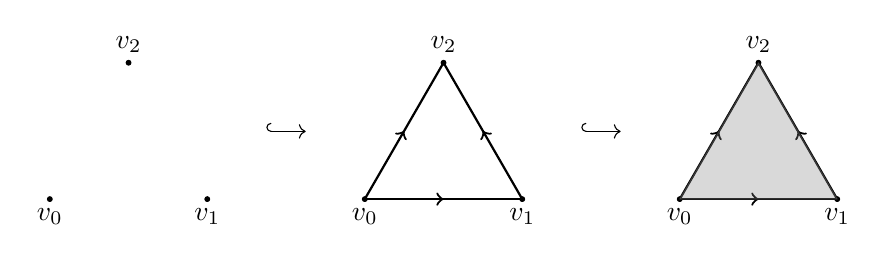
\begin{tikzpicture}[line join = round, line cap = round]

                        % first-simplex
                        \coordinate [label=below:$v_0$] (0) at (0,0);
                        \coordinate [label=below:$v_1$] (1) at (2,0);
                        \coordinate [label=above:$v_2$] (2) at (1,{sqrt(3)});

                         % second-simplex
                        \coordinate [label=below:$v_0$] (3) at (4,0);
                        \coordinate [label=below:$v_1$] (4) at (6,0);
                        \coordinate [label=above:$v_2$] (5) at (5,{sqrt(3)});

                        % third-simpex
                        \coordinate [label=below:$v_0$] (6) at (8,0);
                        \coordinate [label=below:$v_1$] (7) at (10,0);
                        \coordinate [label=above:$v_2$] (8) at (9,{sqrt(3)});

                        \begin{scope}[decoration={markings,mark=at position 0.5 with
                            {\arrow{to}}}]
                            % first-simplex
                            \draw[fill] (0) circle [radius=0.03];
                            \draw[fill] (1) circle [radius=0.03];
                            \draw[fill] (2) circle [radius=0.03];
                            \draw [thin, right hook->] (2.75, 0.86) -- (3.25, 0.86);
                            % second-simplex
                            \draw[fill] (3) circle [radius=0.03];
                            \draw[fill] (4) circle [radius=0.03];
                            \draw[fill] (5) circle [radius=0.03];
                            \draw[thick, postaction={decorate}] (3)--(4);
                            \draw[thick, postaction={decorate}] (3)--(5);
                            \draw[thick, postaction={decorate}] (4)--(5);
                           \draw [thin, right hook->] (6.75, 0.86) -- (7.25, 0.86);
                           % third-simpex
                            \draw[fill] (6) circle [radius=0.03];
                            \draw[fill] (7) circle [radius=0.03];
                            \draw[fill] (8) circle [radius=0.03];
                            \draw[thick, postaction={decorate}] (6)--(7);
                            \draw[thick, postaction={decorate}] (6)--(8);
                            \draw[thick, postaction={decorate}] (7)--(8);
                            \filldraw[opacity=.3, gray] (6) --  (7) --  (8) -- cycle;
                        \end{scope}

                    \end{tikzpicture}

            $C_\bullet^0  \longrightarrow   C_\bullet^1   \longrightarrow C_\bullet^2$  \\~\\


    \end{center}

    Maps between complexes:
    \[
        \begin{tikzcd}[ampersand replacement=\&]
                \& C_\bullet^0   \arrow[rr]                                     \&  \& C_\bullet^1 \arrow[rr]                               \&  \& C_\bullet^2                                                                 \\ \\
                \& 0 \arrow[d]                                         \&  \& 0 \arrow[d]                                         \&  \& 0 \arrow[d]                                                                 \\
                2 \& 0 \arrow[rr] \arrow[d, "\partial^0_2=0"]            \&  \& 0 \arrow[rr] \arrow[d, "\partial^1_2=0"]            \&  \& \mathbb{Z} \arrow[d, "\partial_2^2 = {\begin{pmatrix} 1 \\ 1  \\  -1  \end{pmatrix}}"] \\
                1 \& 0 \arrow[d, "\partial^0_1=0"] \arrow[rr]            \&  \& \mathbb{Z}^3 \arrow[rr] \arrow[d, "\partial_1^1 = \partial_1^2"]                   \&  \& \mathbb{Z}^3 \arrow[d, "\partial_1^2 = {\begin{pmatrix} -1 & 0 & -1 \\ 1 & -1 & 0 \\ 0 & 1 & 1 \end{pmatrix}}"]                                                      \\
                0 \& \mathbb{Z}^3 \arrow[d, "\partial^0_0=0"] \arrow[rr] \&  \& \mathbb{Z}^3 \arrow[rr] \arrow[d, "\partial^1_0=0"] \&  \& \mathbb{Z}^3 \arrow[d, "\partial^2_0=0"]                                    \\
                \& 0                                                   \&  \& 0                                                   \&  \& 0
    \end{tikzcd}
\]
        Induced maps on homology:
       \[
     \begin{tikzcd}[ampersand replacement=\&]
            \& H(C_\bullet^0)   \arrow[rr]                                     \&  \& H(C_\bullet^1) \arrow[rr]                               \&  \& H(C_\bullet^2)                                                                 \\ \\
            \& 0 \arrow[d]                                         \&  \& 0 \arrow[d]                                         \&  \& 0 \arrow[d]                                                                 \\
            2 \& 0 \arrow[rr] \arrow[d]            \&  \& 0 \arrow[rr] \arrow[d]            \&  \& 0 \arrow[d] \\
            1 \& 0 \arrow[d] \arrow[rr]            \&  \& \mathbb{Z} \arrow[rr] \arrow[d]                   \&  \& 0 \arrow[d]                                              \\
            0 \& \mathbb{Z}^3 \arrow[d] \arrow[rr] \&  \& \mathbb{Z} \arrow[rr] \arrow[d] \&  \& \mathbb{Z} \arrow[d]                                    \\
            \& 0                                                   \&  \& 0                                                   \&  \& 0
    \end{tikzcd}
         \]

     \chapter{Singular Homology and Homotopy Invariance}
        \label{SingularHomology}


     In the previous chapter, we considered a parameterization of a space by simplexes, where the maps $\sigma_\alpha: \Delta^n \rightarrow X$ had restrictions defined in \ref{Delta-complex}. If we only require that the $\sigma$ map is continous, then by definition that would be a singular $n-simplex$ in a space $X$.
     The lack of other restrictions on the map $\sigma: \Delta^n \rightarrow X$, convey that $\sigma$ does not need to be a `nice` embedding, in fact it can have singularities, where its image does not look like a simplex.

     $C_n(X)$ is a free abelian group with generators the set of singluar $n-simplexes$ in X: the continous maps $\sigma: \Delta^n \rightarrow X$. The elements of $C_n(X)$ are singular $n-chains$ defined as $\sum_i(n_i\sigma_i)$ for $n_i \in \ZZ$. The boundary operator $\partial_n: C_n(x) \rightarrow C_{n-1}(X)$ is defined the same way as in simplicial $n-chains$, by the formula:
     \[
		         \partial_n(\sigma) = \sum\limits_i (-1)^i \sigma | [v_0, ... ,\hat{v_i}, ... , v_n]
              \]
     By preserving the order of the vertices, the $\sigma |[v_0, ... ,\hat{v_i}, ... , v_n]$ is identified with the map $\Delta^{n-1} \rightarrow X$. The proof of lemma \ref{delta2}, $\partial_2 = 0$, holds true also for singular simplexes. Therefore, the singular homology group is defined the same way: $H_n(x) = \ker\partial_n \left/ \Ima \partial_{n+1} \right.$. The elements in the $\ker$ are singular cycles, and the elements in the $\Ima$ singular boundaries. \\

      Let us consider some explicit examples of $C_n(X)$:
      \begin{itemize}
       \item
      For a topological space $X$:
      $C_0(X)$ consists of all maps $\sigma: \Delta^0 \rightarrow X$, which means that $C_0(X)$ is a free group on the points of $X$.
      \item
      If X = $\RR$: $C_1(X)$ consists of all maps $\sigma: \Delta^1 \rightarrow \RR$, which means that $C_0(X)$ is a free group on continuous maps:
      \[
        [0, 1] \simeq \Delta^1 \rightarrow \\R
      \]
      In this case $C_1(X)$ can be considered as a vector space with vectors the maps: $[0, 1] \rightarrow \RR$.
      \end{itemize}

    From the examples above, it is clear that the groups $C_n(X)$ can be so large to the point where the number of singular $n-simplexes$ in a space $X$ is uncountable. It is not easy to see that even in singular homology where $X$ is generated by a finite number of simplexes, $H_n(X)$ should be finite generated for all n, and that $H_n(X)$ should be 0 for $n > dim(X)$.

    At first glance, singular homology seems to be more general than simplicial homology, however if for an arbitrary space X , we define the singular complex $S(X)$ as a $\Delta-complex$ with one $n-simplex \ \Delta_\sigma^n$ for each singular $n-simplex$ $\sigma: \Delta^n \rightarrow X$, then $H_n^\Delta(S(X))$ is the same as $H_n(X)$. In this case singular homology can be viewed as a special case of simplicial homology.


    \section{Homotopy invariance}

    A significant result that can be proven by singluar homology is that if two spaces $X, Y$ are homeomorphic, the singular homology groups are isomorphic $ H_n(X) \simeq H_n(Y)$.

    \emph{More generally},
    A continuous map $f: X \rightarrow Y$ induces a chain map: $f_\#: C_n(X) \rightarrow C_n(Y)$.
    \begin{gather*}
        f_\#(\sigma: \Delta^ n \rightarrow X) = f \circ \sigma \\
                    \xymatrix{
                        \Delta^n  \ar[r]^{\sigma} &
                        X  \ar[r]^{f} & Y  }
    \end{gather*}

    The boundary operator of $f_\#$ is equal to $\partial_n(f \circ \sigma) = f \circ \partial_n(\sigma)$.

    $H_n(f_\#) = f_*: H_n(X) \rightarrow H_n(Y)$ \\

    \par
    If we additionally require $f$ to be a bijection and have a continuous inverse $f^{-1}$, so $f$ is a homeomorphism, then $f_\#: C_n(X) \simeq C_n(Y)$
    \begin{align*}
        \sigma &\mapsto f \circ \sigma \\
        \mu \circ f^{-1} &\mapsfrom \mu
    \end{align*}
    Then the induced singular homology map $f_*: H_n(X) \simeq H_n(Y)$ defines an isomorphism.

    Moreover,
    \begin{gather}
        f_* \ preserves \ composition, (f \circ g)_* = f_* \circ g_* \\
        f_* \ preserves \ the \ identity, id: X \rightarrow Y \ goes \ to \ id_*:  H_n(X) \rightarrow H_n(Y)
    \end{gather}

    \emph{Category Theory Interpretation}: \label{functoriality} If we consider $Top$ to be the category of topological spaces where maps are continuous:
    \[{Hom}_{Top}(X, Y) = \{f: X \rightarrow Y, f \ is \ continous\},\] and $Ab$ the category of abelian groups were maps are group homomorphisms: \[{Hom}_{Ab}(G, H) = \{\phi: G \rightarrow H, \phi \ is \ group \ homomorphism\}\] then for each $n \geq 0$:
     \begin{align*}
        H_n: Top &\rightarrow Ab \\
            X &\rightsquigarrow H_n(X) \\
        f: X \rightarrow Y &\rightsquigarrow f_*:  H_n(X) \rightarrow H_n(Y)
    \end{align*}
    $H_n$ is a functor and (2.1) (2.2) hold.  \\
    If we also consider the category, Homotopic Topology $HoTop$ of topological spaces where maps are continuous up to homotopy, then we obtain the following commutative diagram:

	\[
		\xymatrix{
			Top  \ar[r]^{H_n} \ar[d]
			& Ab  \\
			HoTop \ar@{.>}[ur] }
	\]

	\[ {Hom}_{HoTop}(X, Y) = {Hom}_{Top}(X, Y) \left/ \simeq \right. \]

    \emph{Remark}: The continous maps $f, g: X \rightarrow Y$ are homotopic if
    \begin{align*}
     &\exists \ H: X \times [0, 1] \rightarrow Y , \\
     &for \ x \in X \ and \ t \in [0, 1]: H(x, t) = H_t(x) \\
     &s.t \ H(x, 0) = f(x) \ and \ H(x, 1) = g(x) \\
     &i.e \ H|_{x \times \{0\}} = f \ and \ H|_{x \times \{1\}} = g
     \end{align*}

     Let us consider some explicit homotopic maps:

     \begin{itemize}
      \item $f, g: \RR \rightarrow \RR$ where $f = id, f(x) = x \ \forall \ x \in X$, and $g = 0, \ g(x) = 0 \ \forall \ x \in X$ \\
      $H: \RR \times [0, 1] \rightarrow \RR$ \\
      $H(x, t) = (1-t)x$, clearly $H(x, 0) = x$ and $H(x, 1) = 0$
      \item $f, g: S^1 \rightarrow \RR^2$ where $f \ is \ an \ inclusion, f(x,y) = (x,y) \ \forall \ (x, y) \in S^1$, and $g = 0, \ g(x,y) = 0 \ \forall \ (x, y) \in S^1$ \\
      $H: S^1 \times [0, 1] \rightarrow \RR^2$ \\
      $H(x, y, t) = (1-t)\langle x, y \rangle$, clearly $H(x, y, 0) = \langle x, y \rangle$ and $H(x, y, 1) = 0$
     \end{itemize}

     \label{homotopicSpaces}If $f, g: X \rightarrow Y$ are homotopic, then the induced maps on homology
     $f_*, g_*: H_n(X) \rightarrow H_n(X)$, are the same $f_* = g_* \ \forall{n}$

     Define $p_n: C_n^{sing}(X) \rightarrow C_{n+1}^{sing}(Y) $ s.t $f_\# - g_\# = \partial p + p\partial$ \\

        \begin{equation*}
                    \xymatrix@+3em{
                        & C_{n + 1}(X)
                            \ar[r]^{\partial_{n + 1}}
                            \ar@<0.5ex>[d]^{g_{n + 1}}
                            \ar@<-0.5ex>[d]_{f_{n + 1}}
                        & C_n(X)
                            \ar[r]^{\partial_n}
                            \ar@<0.5ex>[d]^{g_n}
                            \ar@<-0.5ex>[d]_{f_n}
                            \ar[dl]|*+<1ex,1ex>{\scriptstyle p_n}
                        & C_{n - 1}(X)
                            \ar@<0.5ex>[d]^{g_{n - 1}}
                            \ar@<-0.5ex>[d]_{f_{n - 1}}
                            \ar[dl]|*+<1ex,1ex>{\scriptstyle p_{n - 1}}
                            \\
                        & C_{n + 1}(Y) \ar[r]^{\delta_{n + 1}}
                        & C_n(Y) \ar[r]^{\delta_n}
                        & C_{n - 1}(Y)
                    }
            \end{equation*}





        For $\sigma: \Delta^n \rightarrow X$ the map $p_n(\sigma): \Delta^{n+1} \rightarrow Y$ should be a continous map. \\
        $H: X \times [0, 1] \rightarrow Y$, $H|_{x \times \{0\}} = f \ and \ H|_{x \times \{1\}} = g $
        \[
         \xymatrix{
                        \Delta^n \times[0, 1] \ar[r]^{\sigma \times 1} &
                        {X \times [0, 1]} \ar[r]^{H} & Y  }
        \]
        The idea is to write $\Delta^n \times[0, 1]$ as union of $\Delta^{n+1}$.
        Let us consider some explicit examples of the $p$ maps:
        \begin{itemize}
         \item $p_0: C_0(X) \rightarrow C_1(Y)$ \\
         $p_0(\sigma) = H_0(\sigma \times 1) |_{[v_0w_0]}: \Delta^1 \rightarrow Y$ \\
         We can parameterize $\Delta^1$, as $\Delta^1 = \{ (t_0, t_1) | \ t_0 + t_1 = 1, \ t_0, t_1 \geq 1 \}$ \\
         $\Delta^1 = \{1\} \subseteq \RR$, $\sigma(1) = q$ \\
         \begin{align*}
             \Delta^0 \times [0, 1] &\simeq \Delta^{1} \\
             \{1\} \times \{t\} &\mapsto (1-t, t) \\
             \sigma \times 1: (1, t) &\mapsto (\sigma(1), t) \\
            H_0( \sigma \times 1): (1, t) &\mapsto H(q, t), \ where \ H(q, 0) = f(q), \  H(q, 1) = g(q)\\
         \end{align*}
         \item $p_1: C_1(X) \rightarrow C_2(Y)$ \\
         $p_1(\sigma) = \sum_{i = 0}^1 H_0(\sigma \times 1) |_{[v_0 ... w_1]} = H_0(\sigma \times 1) |_{[v_0 w_0 w_1]} - H_0(\sigma \times 1) |_{[v_0 v_1 w_1]}$ \\
         \begin{align*}
             \Delta^1 \times [0, 1] &\simeq [0, 1] \times [0, 1] \\
             ((t_0, t_1), t) &\mapsto (t_0, t) \\
             \sigma \times 1: (1, t) &\mapsto (\sigma(1), t) \\
            H_0( \sigma \times 1): (1, t) &\mapsto H(q, t), \ where \ H(q, 0) = f(q), \  H(q, 1) = g(q)\\
         \end{align*}
                 \begin{equation*}
                    \xymatrix@+3em{
                        & C_2(X)
                            \ar[r]^{\partial_2}
                        & C_1(X)
                            \ar[r]^{\partial_1}
                            \ar@<0.5ex>[d]^{g}
                            \ar@<-0.5ex>[d]_{f}
                            \ar[dl]|*+<1ex,1ex>{\scriptstyle p_1}
                        & C_0(X)
                            \ar[r]^{\partial_0}
                            \ar[dl]|*+<1ex,1ex>{\scriptstyle p_{0}}
                        & 0
                            \\
                        & C_2(Y) \ar[r]^{\delta_{2}}
                        & C_1(Y) \ar[r]^{\delta_1}
                        & C_0(Y) \ar[r]^{\delta_0}
                        & 0
                    }
            \end{equation*}

            From the diagram above: $\delta_2p_1 + p_0\partial_1: C_1(X) \rightarrow C_1(Y)$ \\
             \begin{align*}
                (p_0 \circ \partial_1)(\sigma) &= p_0(\sigma|_{[v_1]} - \sigma|_{[v_0]}) \\
                &= H_0(\sigma \times 1)|_{[v_1w_1]} - H_0(\sigma \times 1)|_{[v_0w_0]} \\
                &= H_0(\sigma|_{[v_1]} \times 1)|_{[v_1w_1]} - H_0(\sigma|_{[v_0]} \times 1)|_{[v_0w_0]} \\
                &= H_0(\sigma \times 1)|_{[v_1] \times [0, 1]} - H_0(\sigma \times 1)|_{[v_0] \times [0, 1]} \\
           \end{align*}
           \begin{align*}
                (\delta_2 \circ p_1)(\sigma) &= \delta_2(H_0(\sigma \times 1)|_{[v_0w_0w_1]} - H_0(\sigma \times 1)|_{[v_0v_1w_1]}) \\
                &= H_0 (\sigma \times 1)|_{[w_0w_1]} - H_0 (\sigma \times 1)|_{[v_0w_1]} + H_0 (\sigma \times 1)|_{[v_0w_0]} \\
                &- H_0 (\sigma \times 1)|_{[v_1w_1]} + H_0 (\sigma \times 1)|_{[v_0w_1]} - H_0 (\sigma \times 1)|_{[v_0v_1]} \\
           \end{align*}
         So , $(\delta_2p_1 + p_0\partial_1)(\sigma) = H_0 (\sigma \times 1)|_{[w_0w_1]} - H_0 (\sigma \times 1)|_{[v_0v_1]} = g \circ \sigma - f \circ \sigma = (g-f) \circ \sigma$ \\
         \[ \Rightarrow \delta_2p_1 + p_0\partial_1 = g-f \]
        \end{itemize}


     \begin{thm} \label{homotopicChainSameHomology}
      If two chain maps $f_\bullet, g_\bullet: (C_\bullet, \partial) \rightarrow (D_\bullet, \delta) $ are chain-homotopic then they induce the same homomorphism on homology:
     \end{thm}
     More explicitly:
                \begin{equation*}
                    \xymatrix@+3em{
                    {\dots} \ar[r]^{\partial_{n + 2}}
                        & C_{n + 1}
                            \ar[r]^{\partial_{n + 1}}
                            \ar@<0.5ex>[d]^{g_{n + 1}}
                            \ar@<-0.5ex>[d]_{f_{n + 1}}
                            \ar[dl]|*+<1ex,1ex>{\scriptstyle p_{n + 1}}
                        & C_n
                            \ar[r]^{\partial_n}
                            \ar@<0.5ex>[d]^{g_n}
                            \ar@<-0.5ex>[d]_{f_n}
                            \ar[dl]|*+<1ex,1ex>{\scriptstyle p_n}
                        & C_{n - 1}
                            \ar[r]^{\partial_{n - 1}}
                            \ar@<0.5ex>[d]^{g_{n - 1}}
                            \ar@<-0.5ex>[d]_{f_{n - 1}}
                            \ar[dl]|*+<1ex,1ex>{\scriptstyle p_{n - 1}}
                        & {\dots}
                            \ar[dl]|*+<1ex,1ex>{\scriptstyle p_{n - 2}}\\
                    {\dots} \ar[r]^{\delta_{n + 2}}
                        & D_{n + 1} \ar[r]^{\delta_{n + 1}}
                        & D_n \ar[r]^{\delta_n}
                        & D_{n - 1} \ar[r]^{\delta_{n - 1}}
                        & {\dots}
                    }
            \end{equation*}



            \begin{align*}
                  H_n(f) &:  H_n(C_\bullet) \rightarrow H_n(D_\bullet)  \\
                  H_n(f) &: [x] \mapsto [f_n(x)]
                \end{align*}

        If $f_n - g_n = \delta_{n+1}p_n + p_{n-1}\partial_n \Rightarrow H_n(f) = H_n(g)$

        \emph{Proof}: Let us proof that the maps $f_n, g_n$ induce the same homology.\\
        For any $x \in \ker\partial_n \Rightarrow \partial_nx = 0$, \\
        $(f_n - g_n)(x) = \delta_{n+1}p_n(x) + p_{n-1}\delta_n(x) = \delta_{n+1}(p_n(x)) \in \Ima(\partial_{n+1})$ \\
        $\Rightarrow (f_n - g_n)(x) \in \Ima(\partial_{n+1})$
            \[
				\left|
				  \begin{array}{l}
				  	H_n(f) ([x]) = [f_n(x)] \\
				  	H_n(g) ([x]) = [g_n(x)] \\
				  \end{array} \Rightarrow [f_n(x)] - [g_n(x)] = [f_n(x) - g_n(x)] = [\delta_{n+1}p_n(x)] = [0]
				\right.
			\]
			since $\delta_{n+1}(p_n(x)) \in \Ima(\partial_{n+1})$. \\
			So, $[f_n(x)] = [g_n(x)] \Rightarrow H_n(f) = H_n(g) \qed$ \\

        \begin{Ex}
         Let $X$ be a $1-simplex$ and $Y$ a $2-simplex$:
         \begin{center}


                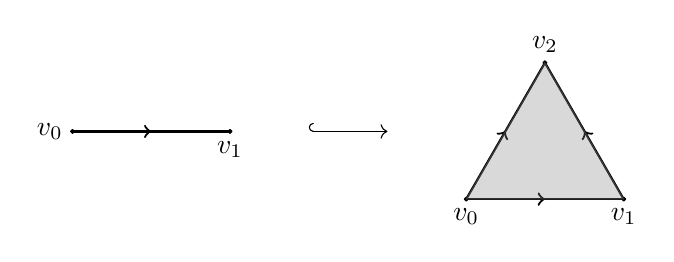
\begin{tikzpicture}[line join = round, line cap = round]

                  1-simplex
                  \coordinate [label=left:$v_0$] (1) at (1,0.86);
                  \coordinate [label=below:$v_1$] (2) at (3,0.86);

                  2-simplex
                  \coordinate [label=below:$v_0$] (3) at (6,0);
                  \coordinate [label=below:$v_1$] (4) at (8,0);
                  \coordinate [label=above:$v_2$] (5) at (7,{sqrt(3)});

                  \begin{scope}[decoration={markings,mark=at position 0.5 with {\arrow{to}}}]
                   \draw [thin, right hook->] (4, 0.86) -- (5, 0.86);
                    1-simplex
                    \draw[fill] (1) circle [radius=0.025];
                    \draw[fill] (2) circle [radius=0.025];
                    \draw[thick, postaction={decorate}] (1)--(2);
                    2-simplex
                    \draw[fill] (3) circle [radius=0.025];
                    \draw[fill] (4) circle [radius=0.025];
                    \draw[fill] (5) circle [radius=0.025];
                    \draw[thick, postaction={decorate}] (3)--(4);
                    \draw[thick, postaction={decorate}] (3)--(5);
                    \draw[thick, postaction={decorate}] (4)--(5);
                     \filldraw[opacity=.3, gray] (3) --  (4) --  (5) -- cycle;
                  \end{scope}

                \end{tikzpicture}
                \end{center}
          \begin{equation*}
                    C_\bullet(X, \partial):
                    \xymatrix@+3em{
                        & 0
                            \ar[r]^{\partial_2}
                        & \ZZ
                            \ar[r]^{\partial_1}
                        & \ZZ^{\oplus^2}
                            \ar[r]^{\partial_0 = 0}
                        & 0
                    }
            \end{equation*}
         \begin{equation*}
                    D_\bullet(Y, \delta):
                    \xymatrix@+3em{
                        & \ZZ
                            \ar[r]^{\delta_2}
                        & \ZZ^{\oplus^3}
                            \ar[r]^{\delta_1}
                        & \ZZ^{\oplus^3}
                            \ar[r]^{\delta_0 = 0}
                        & 0
                    }
            \end{equation*}

        Let's introduce maps on the chain complexes:
         \begin{align*}
        f_n: C_n(X, \partial) \rightarrow C_n^{\prime}(Y, \delta) \\
        g_n: C_n(X, \partial) \rightarrow C_n^{\prime}(Y, \delta)
         \end{align*}

         \begin{equation*}
                    \xymatrix@+3em{
                        & 0
                            \ar[r]^{\partial_2}
                        & \ZZ
                            \ar[r]^{\partial_1 = \left[\begin{smallmatrix} -1 \\ 1 \end{smallmatrix}\right]}
                            \ar@<-0.5ex>[d]_{f_1 = \left[\begin{smallmatrix}0 \\
                            0  \\
                            1 \\ \end{smallmatrix}\right]}
                            \ar@<0.5ex>[d]^{g_1 = \left[\begin{smallmatrix} 0 \\
                                1 \\
                                0 \\ \end{smallmatrix}\right]}
                            \ar[dl]_{\scriptstyle p_1 = id}
                        & \ZZ^{\oplus^2}
                            \ar[r]^{\partial_0 = 0}
                            \ar@<-0.5ex>[d]_{f_0 = \left[\begin{smallmatrix}1 & 0 \\
                            0 & 0 \\
                            0 & 1 \\ \end{smallmatrix}\right]}
                            \ar@<0.5ex>[d]^{g_0 = \left[\begin{smallmatrix}1 & 0 \\
                            0 & 1 \\
                            0 & 0 \\ \end{smallmatrix}\right]}
                            \ar[dl]
                        & 0
                            \\
                        & \ZZ \ar[r]_{\delta_2 = \left[\begin{smallmatrix}1  \\
                            -1 \\
                            1 \\ \end{smallmatrix}\right]}
                        & \ZZ^{\oplus^3}
                            \ar[r]_{\delta_1 = \left[\begin{smallmatrix}0 & -1 & -1 \\
                                -1 & 0 & 1 \\
                                1 & 1 & 0 \\ \end{smallmatrix}\right]}
                        & \ZZ^{\oplus^3}
                        \ar[r]_{\delta_0 = 0}
                        & 0
                    }
            \end{equation*}
            We can define $p_0 = \begin{bmatrix} 0 & 1 \\ 0 & 0 \\ 0 & 0 \\ \end{bmatrix}$
            and $p_1 = id_\ZZ$ \\
            For $n = 0$:
             \begin{align*}
            f_0 - g_0 &= \begin{bmatrix} 1 & 0 \\
                            0 & 0 \\
                            0 & 1 \\ \end{bmatrix} -
            \begin{bmatrix}1 & 0 \\
                            0 & 1 \\
                            0 & 0 \\ \end{bmatrix} =
                            \begin{bmatrix}0 & 0 \\
                            0 & -1 \\
                            0 & 1 \\ \end{bmatrix} \\
           \delta_{1}p_0 + 0 \circ \partial_0 &= \begin{bmatrix} 0 & -1 & -1 \\
                                -1 & 0 & 1 \\
                                1 & 1 & 0 \\ \end{bmatrix} \begin{bmatrix} 0 & 1 \\ 0 & 0 \\ 0 & 0 \\ \end{bmatrix} = \begin{bmatrix} 0 & 0 \\
                            0 & -1 \\
                            0 & 1 \\ \end{bmatrix}
            \end{align*}

         For the choice of the maps $p_0, f_0, g_0$: $f_0 \simeq g_0 \rightarrow$ homotopic equivalent \\
         For $n = 1$:
           \begin{align*}
            f_1 - g_1 &= \begin{bmatrix} 0 \\
                            0  \\
                            1 \\  \end{bmatrix} -
            \begin{bmatrix} 0 \\
                            1  \\
                            0 \\ \end{bmatrix} =
                            \begin{bmatrix}0 \\
                            -1 \\
                            1 \\ \end{bmatrix} \\
           \delta_{2}p_1 + p_0 \circ \partial_1 &= \begin{bmatrix} 1  \\
                            -1 \\
                            1 \\  \end{bmatrix} \begin{bmatrix} 1 \\ \end{bmatrix}
                            + \begin{bmatrix} 0 & 1 \\ 0 & 0 \\ 0 & 0 \\   \end{bmatrix} \begin{bmatrix} -1 \\ 1 \end{bmatrix}
                            = \begin{bmatrix} 0 \\
                            -1 \\
                            1 \\\end{bmatrix}
            \end{align*}
             For the choice of the maps $p_1, p_0, f_1, g_1$: $f_1 \simeq g_1 \rightarrow$ homotopic equivalent \\
             By theorem \ref{homotopicChainSameHomology}, $H_0(f) = H_0(g)$ and $H_1(f) = H_1(g)$. \\
             More precisely, $H_0(f) = H_0(g) = id_\ZZ$ and $H_1(f) = H_1(g) = 0$, since
             $H_0(X) = H_0(Y) = \\Z$ and $H_n(X) = H_n(Y) = 0 \ \forall \ n > 0$
        \end{Ex}
        \begin{Lemma}
         A chain complex $(C_\bullet, \partial)$ is contractable if $ id_C \ is \ homotopic \ equivalent \ to \ 0_C$
        \end{Lemma}
        If $ id_C \simeq 0_C$, then $H_n(C_\bullet) = 0 \ \forall n$ \\
        Examples:
        \begin{itemize}
         \item $C_\bullet: \ \xymatrix{
                        \ZZ  \ar[r]^{0} &
                        \ZZ  \ar[r] & 0  }$ \\
        $H_0(C_\bullet) = \ZZ = H_1(C_\bullet)$ implies that $C_\bullet$ is not contractable
        \item $D_\bullet: \ \xymatrix{
                        \ZZ  \ar[r]^{2} &
                        \ZZ  \ar[r] & 0  }$ \\
        $H_0(D_\bullet) = \ZZ / 2\ZZ$, $H_1(D_\bullet) = 0$ implies that $D_\bullet$ is not contractable
        \item $E_\bullet: \ \xymatrix{
                        \ZZ  \ar[r]^{1} &
                        \ZZ  \ar[r] & 0  }$ \\
        $H_0(E_\bullet) = 0 = H_1(E_\bullet) \Rightarrow$ need to check that $ id_E \simeq 0_E$

        \begin{equation*}
                    \xymatrix@+3em{
                        & 0
                            \ar[r]
                        & \ZZ
                            \ar[r]^{\partial_1 = 1}
                            \ar[d]|*+<1ex,1ex>{\scriptstyle id - 0}
                            \ar[dl]|*+<1ex,1ex>{\scriptstyle p_1}
                        & \ZZ
                            \ar[r]^{\partial_0 = 0}
                             \ar[d]|*+<1ex,1ex>{\scriptstyle id - 0}
                            \ar[dl]|*+<1ex,1ex>{\scriptstyle p_{0}}
                        & 0
                            \\
                        & 0 \ar[r]
                        & \ZZ \ar[r]^{\partial_1 = 1}
                        & \ZZ \ar[r]^{\partial_0 = 0}
                        & 0
                    }
            \end{equation*}
        We can assign $p_0 = id$, $p_1 = 0$. \\
        For a cycle $\sigma  \in E_1 = \ZZ$: \\
        $(\partial_2p_1 + p_0\partial_1)(\sigma) = \partial_2p_1(\sigma) + p_0\partial_1(\sigma) = 0 + \sigma = \sigma = id - 0(\sigma) \Rightarrow id_E \simeq 0_E \Rightarrow (E_\bullet, \partial)$ is contractable

        \item $F_\bullet: \ \xymatrix{
                        \dots  \ar[r]^{2} &
                        \ZZ/4  \ar[r]^{2} &
                        \ZZ/4  \ar[r]^{\partial = 2} &
                        \ZZ/4  \ar[r]^{2} &
                        \ZZ/4  \ar[r]^{2} & \dots  }$ \\
        $\ker\partial = \Ima\partial = (2) \Rightarrow H_n(F_\bullet) = 0 \ \forall \ n \Rightarrow$ need to check that $ id_F \simeq 0_F$

        \begin{equation*}
                    \xymatrix@+3em{
                        & \dots
                            \ar[r]^{2}
                        & \ZZ/4
                            \ar[r]^{2}
                            \ar[d]|*+<1ex,1ex>{\scriptstyle id - 0}
                            \ar[dl]|*+<1ex,1ex>{\scriptstyle p_1}
                        & \ZZ/4
                            \ar[r]^{2}
                             \ar[d]|*+<1ex,1ex>{\scriptstyle id - 0}
                            \ar[dl]|*+<1ex,1ex>{\scriptstyle p_{0}}
                        &  \dots
                            \\
                        & \dots \ar[r]^{2}
                        & \ZZ/4 \ar[r]^{2}
                        & \ZZ/4 \ar[r]^{2}
                        & \dots
                    }
            \end{equation*}
        In $\ZZ / 4$ we have four classes $\overline{0}, \overline{1}, \overline{2}, \overline{4}$.
        The boundary operator $\partial = mult(2)$ maps the four classes only in two maps $\overline{0}, \overline{2}$. So, the $\partial$ cannot be surjective. \\
        For a cycle $\sigma \in \ZZ / 4$: \\
        Since $((2)p_1 + p_0(2))(\sigma) \in (2), \  ((2)p_1 + p_0(2))(\sigma) \neq \sigma \Rightarrow (F_\bullet, \partial)$ is not contractable
        \end{itemize}

        \begin{thm} \label{homotopic}
         Given topological spaces $X, Y$ with maps $f: X \rightarrow Y$ and $g: Y \rightarrow X$ \\
%          and maps of complexes: $f_\#: C_n^{sing}(X) \rightarrow C_n^{sing}(Y) $ and $g_\#: C_n^{sing}(Y) \rightarrow C_n^{sing}(X) $: \\
         If
         \begin{align*}
         f \circ g \simeq id_Y \\
         g \circ f \simeq id_X
         \end{align*}
         where $\simeq$ denotes homotopic equivalence, then
        \[
                    \xymatrix{
                        H_n(X) \ar@/^/[rr]|{f_*}
                        && H_n(Y) \ar@/^/[ll]|{g_*} }
                       \quad  \forall \ n \in \ZZ
          \] $H_n(X)$ is isomorphic to $H_n(Y)$, $ \Rightarrow f_* = (g_*)^{-1} $where $f_*, g_*$ are the induced maps on homology.
        \end{thm}
        \begin{Ex}
         Let $X$ be the n-dimensional sphere and $Y$ the (n+1)-dimensional real coordinate space without the origin, $X = S^n$ and $Y = \RR^{n+1} / \{0\}$
         \[
          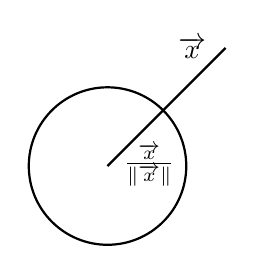
\begin{tikzpicture}[>=stealth',x=1cm,y=1cm]
                \coordinate (A) at (0,0);
                \coordinate (B) at (1.5,1.5);

                \draw[thick, -] (A)--(B);
                \draw[thick, -] (A) circle [radius=1];

                \node at (A) {};
                \node[label={left:$\overrightarrow{x}$}] at (B) {};

                \tkzInterLC[R](A,B)(A,0.75cm) % line (A,B) and circle(A,2cm)
                \tkzGetPoints{E}{F} % intersection points
                \node[label={below:$\frac{\overrightarrow{x}}{\lVert \overrightarrow{x} \rVert}$}] at (F) {};
             \end{tikzpicture}
            \]
         \begin{align*}
         &f: S^n \hookrightarrow \RR^{n+1} / \{0\} \ is \ the  \ usual \ inclusion \\
         &g: \RR^{n+1} / \{0\}  \rightarrow S^n \ s.t \ g(\overrightarrow{x}) = \frac{\overrightarrow{x}}{\lVert \overrightarrow{x} \rVert}
         \end{align*}

         Clearly, $g \circ f \simeq id_S^n$ while $f \circ g: \overrightarrow{x} \mapsto \frac{\overrightarrow{x}}{\lVert \overrightarrow{x} \rVert} \neq id_{\RR^{n+1} / \{0\}}$ \\
         Let's prove that $f \circ g$ is homotopic equivalent to $id_{\RR^{n+1} / \{0\}}$:
         We can construct a function
         \begin{align*}
            F: [0, 1] &\times \RR^{n+1} / \{0\}  \longrightarrow \RR^{n+1} / \{0\} \\
            F(t, \overrightarrow{x}) &= (t( f \circ g) + (1-t)1_{\RR^{n+1} / \{0\}})\overrightarrow{x} \\
            &= t(\frac{\overrightarrow{x}}{\lVert \overrightarrow{x} \rVert}) + (1-t)\overrightarrow{x}
         \end{align*}
         Clearly, $F(0, \overrightarrow{x}) = \overrightarrow{x} = id_{\RR^{n+1} / \{0\}}$  and
         $F(1, \overrightarrow{x}) = (\frac{\overrightarrow{x}}{\lVert \overrightarrow{x} \rVert}) = f \circ g$. \\
         So, $f \circ g \simeq id_{\RR^{n+1} / \{0\}}$, and by theorem \ref{homotopic} $\Rightarrow f_* = (g_*)^{-1}$.
        \end{Ex}
        \begin{Ex}
         Let $X$ be a $1-simplex$ and $Y$ a $0-simplex$:
          \begin{equation*}
                    C_\bullet(X, \partial):
                    \xymatrix@+3em{
                        & 0
                            \ar[r]^{\partial_2}
                        & \ZZ
                            \ar[r]^{\partial_1}
                        & \ZZ^{\oplus^2}
                            \ar[r]^{\partial_0 = 0}
                        & 0
                    }
            \end{equation*}
         \begin{equation*}
                    C_\bullet^{\prime}(Y, \partial^{\prime}):
                    \xymatrix@+3em{
                        & 0
                            \ar[r]^{0}
                        & 0
                            \ar[r]^{\partial_1^\prime = 0}
                        & \ZZ
                            \ar[r]^{\partial_0^\prime = 0}
                        & 0
                    }
            \end{equation*}

        Let's introduce maps on the chain complexes:
         \begin{align*}
        f_n: C_n(X, \partial) \rightarrow C_n^{\prime}(Y, \partial^{\prime}) \\
        g_n: C_n^{\prime}(Y, \partial^{\prime}) \rightarrow C_n(X, \partial)
         \end{align*}

         \begin{equation*}
                    \xymatrix@+3em{
                        & 0
                            \ar[r]^{\partial_2}
                        & \ZZ
                            \ar[r]^{\partial_1}
                            \ar[d]|*+<1ex,1ex>{\scriptstyle 0}
                            \ar[dl]_{\scriptstyle p_1}
                        & \ZZ^{\oplus^2}
                            \ar[r]^{\partial_0 = 0}
                            \ar@<0.5ex>[d]^{f_0 = \left[\begin{smallmatrix}1 & 1 \end{smallmatrix}\right]}
                            \ar[dl]_{\scriptstyle p_{0}}
                        & 0
                            \\
                        & 0 \ar[r]^{0}
                        & 0 \ar[r]^{\partial_1^\prime = 0}
                        & \ZZ
                        \ar[r]^{\partial_0^\prime = 0}
                        \ar@<0.5ex>[u]^{\left[\begin{smallmatrix} 1 \\ 0 \end{smallmatrix}\right] = g_0}
                        & 0
                    }
            \end{equation*}
            For $n = 0$:
             \begin{align*}
            &f_0 \circ g_0 = \begin{bmatrix} 1 & 1 \end{bmatrix} \begin{bmatrix} 1 \\ 0 \end{bmatrix} = id_\ZZ \\
            &g_0 \circ f_0 = \begin{bmatrix} 1 \\ 0 \end{bmatrix} \begin{bmatrix} 1 & 1 \end{bmatrix} = \begin{bmatrix} 1 & 1 \\ 0 & 0 \end{bmatrix} \neq id_{\ZZ^{\oplus^2}}
         \end{align*}

         Let's prove that $g_0 \circ f_0$ is homotopic equivalent to $id_{\ZZ^{\oplus^2}}$:\\
         For an arbitrary element
         $\begin{bmatrix} x \\ y \end{bmatrix} \in \ZZ^{\oplus^2}$: \\
         $(g_0 \circ f_0 - id_{\ZZ^{\oplus^2}})\begin{bmatrix} x \\ y \end{bmatrix} =
         \begin{bmatrix} 0 & 1 \\ 0 & -1 \end{bmatrix}\begin{bmatrix} x \\ y \end{bmatrix} = 0 $ and
          $(\partial_1^\prime p_0 + 0 \circ \partial_0) \begin{bmatrix} x \\ y \end{bmatrix} = 0 \Longrightarrow g_0 \circ f_0 \simeq id_{\ZZ^{\oplus^2}}$ \\
%          For $n = 1$:
%          \begin{align*}
%             &f_1 \circ g_1 \simeq id_0 = 0 \\
%             &g_1 \circ f_1 \, is \, not \,  homotopic \, equivalent \, to \, id_\ZZ \; since \; g_1 \circ f_1 = 0
%          \end{align*}
         To be continued and rechecked
        \end{Ex}


        \section{Exact Sequences}

        \begin{defn}
         A sequence of homomorphisms:
                 \[
                 \xymatrix@+3em{
                        & \dots
                            \ar[r]
                        & A_{n+1}
                            \ar[r]^{\alpha_{n+1}}
                        & A_n
                            \ar[r]^{\alpha_n}
                        & A_{n-1}
                            \ar[r]^{\alpha_{n-1}}
                        & \dots }
                    \]

        is $\underline{exact}$ if $ \ker\alpha_n = \Ima\alpha_{n+1} \ \forall \ n $.
        \end{defn}

                 $ \Ima\alpha_{n+1} \subseteq \ker\alpha_n$ is equivalent to $\alpha_n\alpha_{n+1} = 0$ since $(A_\bullet, \alpha)$ is a chain complex.\\
                 \& $ \ker\alpha_n \subset \Ima\alpha_{n+1} \Rightarrow H_{n} \ is\ trivial: \ H_{n} = 0 \ \forall \ n $ \\

                Examples of short exact sequences:

                \begin{enumerate}
                \item $ 0 \rightarrow A \xrightarrow{\alpha} B \ is\ exact\ \iff \ker\alpha = 0, \alpha \ is\ injective $
                \item $ A \xrightarrow{\alpha} B \rightarrow 0 \ is\ exact\ \iff \Ima\alpha = B, \alpha \ is\ surjective $
                \item
                  $
                    0 \rightarrow A \xrightarrow{\alpha} B \rightarrow 0 \ is\ exact\ \iff \Ima\alpha = B \ and \ \ker\alpha = \{0\}, \alpha \ is \ an \ isomorphism$
                \item
                  $ 0 \rightarrow A \xrightarrow{\alpha} B \xrightarrow{\beta} C \rightarrow 0 \ is\ exact\ \iff $
                   \begin{enumerate}
                    \item
                     $\ker \alpha = \Ima(0 \rightarrow A) = 0\ \Rightarrow \alpha\ is\ injective$
                    \item
                    $\Ima\beta = C \Rightarrow \beta \ is\ surjective$
                    \item
                    $\ker \beta = \Ima\alpha $

                   \end{enumerate}

                    So, $\beta$  induces an isomorphism $C \simeq \frac{B}{\Ima\alpha}$.
                    $C$ can written as $C \simeq B/A$ if $\alpha$ is an inclusion of A as a subgroup of B.
                \end{enumerate}


                Let us consider a short exact sequence of chain complexes: \\
                \[
                0 \rightarrow A_\bullet \xrightarrow{i} B_\bullet \xrightarrow{\pi} C_\bullet \rightarrow 0
                \]

                $A_\bullet, \ B_\bullet, \ C_\bullet$ are chain complexes and $i, \pi$ are maps between chain complexes where \\
                $\ker \pi = \Ima i, \quad \pi:surjective \ and \ i: injective$\\
                \[
                  \begin{tikzcd}[ampersand replacement=\&]
                    \& \            \& \& 0 \arrow[d]                   \&  \& 0      \arrow[d]                 \&  \& 0 \arrow[d] \\
                    \& A_\bullet: \quad \arrow[rr] \& \& A_n \arrow[rr, "\partial"] \arrow[d, "i_n"] \&  \& A_{n-1} \arrow[rr, "\partial"] \arrow[d, "i_{n-1}"] \&  \& A_{n-2} \arrow[d, "i_{n-2}"] \arrow[rr] \& \& \ \\
                    \& B_\bullet: \quad \arrow[rr] \& \& B_n \arrow[rr, "\partial"] \arrow[d, "\pi_n"] \&  \& B_{n-1} \arrow[rr, "\partial"] \arrow[d, "\pi_{n-1}"] \&  \& B_{n-2} \arrow[d, "\pi_{n-2}"] \arrow[rr] \& \& \ \\
                    \& C_\bullet: \quad \arrow[rr] \& \& C_n \arrow[rr, "\partial"] \arrow[d] \&  \& C_{n-1} \arrow[rr, "\partial"] \arrow[d] \&  \& C_{n-2} \arrow[d] \arrow[rr] \& \& \ \\
                    \& \            \& \& 0                             \&  \& 0                                 \&  \& 0\\
                  \end{tikzcd}
                \]


                The induced sequence on homology: \\
                \begin{align}
                H_n(A_\bullet) \xrightarrow{i_*} H_n(B_\bullet) \xrightarrow{\pi_*} H_n(C_\bullet) \ \forall \  n
                \end{align}
                $\pi \circ i = 0 \Rightarrow \pi_* \circ i_* = 0, \quad H_n(\pi \circ i) = H_n(\pi) \circ H_n(i)$\\
                (2.3) \underline{need not} be a short exact sequence. However, we can create a long exact sequence of homology: \\

                 \begin{align*}
                H_{n+1}(C_\bullet) \xrightarrow{\partial n+1} H_n(A_\bullet) \xrightarrow{i_*} H_n(B_\bullet) \xrightarrow{\pi_*} H_n(C_\bullet) \xrightarrow{\delta} H_{n-1}(A_\bullet) \rightarrow H_{n-1}(B_\bullet) \rightarrow H_{n-1}(C_\bullet) \\
                \end{align*}
                \begin{align*}
                0 \rightarrow \Ima \delta_{n+1} \rightarrow H_n(A) \xrightarrow{i_*} H_n(B) \xrightarrow{\pi_*} H_n(C) \rightarrow \ker \delta_n \rightarrow 0 \\
                \\
                \end{align*}


%                 The short exact sequence of chain complexes above induces a long exact sequence on the homology:
%
%                 \begin{align*}
%                   \cdots \rightarrow H_n(A) \rightarrow H_n(B) \rightarrow H_n(C) \xrightarrow{\delta} H_{n-1}(A) \rightarrow H_{n-1}(B) \rightarrow H_{n-1}(C) \\ \xrightarrow{\delta} H_{n-2}(A) \rightarrow H_{n-2}(B) \rightarrow H_{n-2}(C) \rightarrow \cdots
%                 \end{align*}
                where the $\delta$ map is defined as:
                \begin{align*}
                  \delta: H_n(C) &\rightarrow H_{n-1}(A)\\
                  [c] &\mapsto [a]
                \end{align*}
                For a element $b \in B_n$ there exists $c = \pi_n(b)$ since $\pi$ is onto. \\
                If we apply the boundary map $\partial: B_{n} \rightarrow B_{n-1}$ on $b$, then
                $\partial b \in B_{n-1}$,  $\pi_n(\partial b) = \partial(\pi_n(b)) = 0$\\
                We can take an element $a \in A_{n-1}$ such that $i(a) = \partial(b)$\\
                $
                  \partial (\partial b) = \partial (i(a)) = i(\partial a) \Rightarrow \partial a = 0\ since\ i\ is\ injective \ \Rightarrow \partial b = (0) \in A_{n-1}
                $


                \begin{Ex} Let consider $X$ to be a $1-simplex$ and $Y$ a $2-simplex$ \\

                \begin{center}


                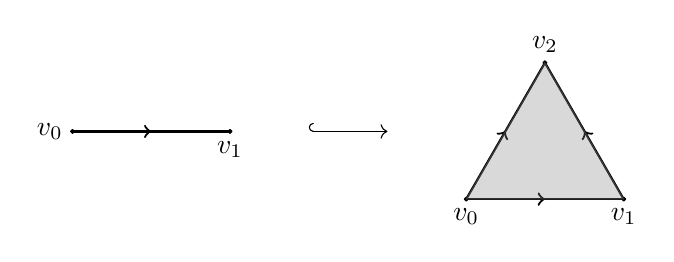
\begin{tikzpicture}[line join = round, line cap = round]

                  1-simplex
                  \coordinate [label=left:$v_0$] (1) at (1,0.86);
                  \coordinate [label=below:$v_1$] (2) at (3,0.86);

                  2-simplex
                  \coordinate [label=below:$v_0$] (3) at (6,0);
                  \coordinate [label=below:$v_1$] (4) at (8,0);
                  \coordinate [label=above:$v_2$] (5) at (7,{sqrt(3)});

                  \begin{scope}[decoration={markings,mark=at position 0.5 with {\arrow{to}}}]
                   \draw [thin, right hook->] (4, 0.86) -- (5, 0.86);
                    1-simplex
                    \draw[fill] (1) circle [radius=0.025];
                    \draw[fill] (2) circle [radius=0.025];
                    \draw[thick, postaction={decorate}] (1)--(2);
                    2-simplex
                    \draw[fill] (3) circle [radius=0.025];
                    \draw[fill] (4) circle [radius=0.025];
                    \draw[fill] (5) circle [radius=0.025];
                    \draw[thick, postaction={decorate}] (3)--(4);
                    \draw[thick, postaction={decorate}] (3)--(5);
                    \draw[thick, postaction={decorate}] (4)--(5);
                     \filldraw[opacity=.3, gray] (3) --  (4) --  (5) -- cycle;
                  \end{scope}

                \end{tikzpicture}
                \end{center}
                A short exact sequence of chain complexes for $X, Y$:

                \[
                  \begin{tikzcd}[ampersand replacement=\&, sep=large]
                        \& \            \&  \& 0 \arrow[d] \&  \& 0 \arrow[d] \& \& \\
                    A_\bullet: \& 0 \arrow[rr] \&  \& \mathbb{Z} \arrow[rr, "\partial = {\left[\begin{smallmatrix}-1\\1\end{smallmatrix}\right]}"] \arrow[d,swap,"i_1 = {\left[\begin{smallmatrix}0\\0\\1\end{smallmatrix}\right]}"] \&  \& \mathbb{Z}^{\oplus^{2}} \arrow[rr] \arrow[d, "i_0 = {\left[\begin{smallmatrix}1&0\\0&0\\0&0\end{smallmatrix}\right]}"] \&  \& 0\\
                    B_\bullet: \& 0 \arrow[rr] \&  \& \mathbb{Z}^{\oplus^{3}} \arrow[rr, "\partial = {\left[\begin{smallmatrix}0&-1&-1\\-1&0&1\\1&1&0\end{smallmatrix}\right]}"] \arrow[d, "\pi_1"] \&  \& \mathbb{Z}^{\oplus^{3}} \arrow[d, "\pi_0"] \arrow[rr] \&  \& 0\\
                    C_\bullet: \& 0 \arrow[rr] \&  \& C_1        \arrow[rr] \arrow[d] \&  \& C_0               \arrow[d] \arrow[rr] \&  \& 0\\
                        \& \            \&  \& 0                               \&  \& 0\\
                  \end{tikzcd}
                \]
                The short exact sequence of complexes induces a long exact sequence on homology:
                \[
                0 \rightarrow H_1(A) \rightarrow H_1(B) \rightarrow H_1(C) \xrightarrow{\delta} H_0(A) \rightarrow H_0(B) \rightarrow H_0(C) \rightarrow 0 \]
                Explicitly, the long exact sequence is:

                \[
                0 \rightarrow 0 \rightarrow \mathbb{Z} \rightarrow H_1(C) \xrightarrow{\delta} \mathbb{Z} \xrightarrow{1} \mathbb{Z} \xrightarrow{\alpha} H_0(C) \rightarrow 0
                \]
                \begin{align*}
                  &\ker(1) = \{0\} = \Ima \delta\\
                  &\ker(\alpha) = \Ima(1) = \mathbb{Z}
                \end{align*}
                \begin{align*}
                  C_1 &= \mathbb{Z}^{\oplus^{3}} / \Ima i_1 \simeq \mathbb{Z}^{\oplus^{2}}\\
                  C_0 &= \mathbb{Z}^{\oplus^{3}} / \Ima i_0 \simeq \mathbb{Z}
                \end{align*}
                The boundary operator between $C_1, C_0$:
                  \begin{align*}
                 &\partial: C_1 \rightarrow C_0 \\
                 &\partial: \begin{bmatrix}
                    a\\b
                  \end{bmatrix}
                  \mapsto (a+b)
                \end{align*}


%                 \begin{align*}
%                   \begin{bmatrix}
%                     1\\0
%                   \end{bmatrix}
%                   \mapsto
%                   \begin{bmatrix}
%                     1\\0\\0
%                   \end{bmatrix}
%                   \begin{bmatrix}
%                     a\\b
%                   \end{bmatrix}
%                   \mapsto (a+b)
%                   \\
%                   \begin{bmatrix}
%                     a\\b
%                   \end{bmatrix}
%                   =
%                   \begin{bmatrix}
%                     a\\-a+a+b
%                   \end{bmatrix}
%                   =
%                   \begin{bmatrix}
%                     a\\-a
%                   \end{bmatrix}
%                   +
%                   \begin{bmatrix}
%                     0\\a+b
%                   \end{bmatrix}
%                 \end{align*}

                \begin{align*}
                  \begin{bmatrix}
                    a\\b
                  \end{bmatrix}
                  =
                  \begin{bmatrix}
                    a\\b\\0
                  \end{bmatrix} mod(\Ima i_1) \xmapsto{\partial = \left[\begin{smallmatrix}0&-1&-1\\-1&0&1\\1&1&0\end{smallmatrix}\right]} \begin{bmatrix}
                    -b\\-a\\a+b
                  \end{bmatrix}
                  =
                  \begin{bmatrix}
                    0\\0\\a+b
                  \end{bmatrix}
                \end{align*}

                \begin{align*}
                  H_1(C) = \left\{\begin{bmatrix}a\\-a\end{bmatrix}\right\} \simeq \mathbb{Z} \\
                  H_0(C) = C_0 / C_0 = 0
                \end{align*}
                \\
                \end{Ex}
                Let us take an example when $Y \subseteq X$ subspace, the short exact sequence of chain complexes is: \\
                \[
                0 \rightarrow C_n(Y) \rightarrow C_n(X) \rightarrow C_n(X) / C_n(Y) \rightarrow 0
                \]
                We get a long exact sequence on homology: \\
                \[ H_n(Y) \rightarrow H_n(X) \rightarrow H_n(X, Y) \xrightarrow{\delta} H_{n-1}(Y) \rightarrow H_{n-1}(X) \rightarrow \cdots \]

                \begin{Ex} Consider $X$ to be the annulus, and the shaded area $Y \subseteq X$
                \[
                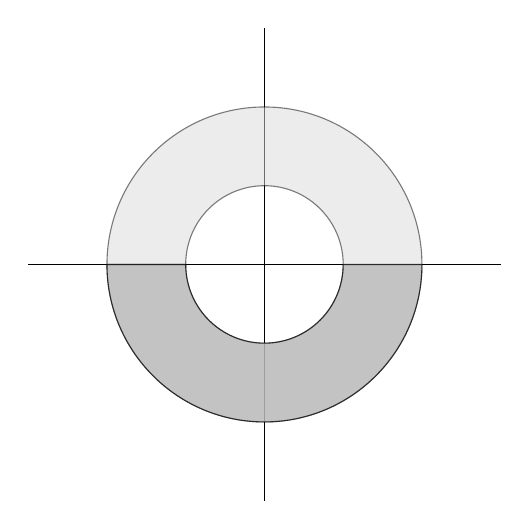
\begin{tikzpicture}
                    \draw (-3,0) -- (3,0);
                    \draw (0,-3) -- (0,3);
                    \filldraw[fill=gray!30,opacity=0.5] (-180:1) arc (-180:180:1) -- (180:2) arc (180:-180:2) -- cycle;
                    \filldraw[fill=black!30,opacity=0.7] (0:1) arc (0:-180:1) -- (-180:2) arc (-180:0:2) -- cycle;

                \end{tikzpicture}
                \]
                    \begin{align*}
                    &X = \{(x,y) | 1 \le x^2 + y^2 \le 2\}\\
                    &Y = \{(x,y) | 1 \le x^2 + y^2 \le 2, y \le 0\}\\
                    &\delta\ :\ H_1(X,Y) \rightarrow H_0(Y)\\
                    &\delta([\sigma]) = [\partial \sigma] = [\sigma(1) - \sigma(0)]
                    \end{align*}
                \end{Ex}

                In "good cases" $H_n(X,Y) = H_n(X/Y)$ \\


                For two topological spaces $Y \subseteq X$ ``pairs of spaces''.\\
                We can construct the following chain complex: \\
                $0 \rightarrow C_n(Y) \xrightarrow{i} C_n(X) \xrightarrow{\pi} C_n(X) / C_n(Y) \rightarrow 0, \quad C_n(X, Y)\ are\ relative\ chains$ \\
                Elements of $C_n$: $\sigma: \Delta^n \rightarrow Y \subseteq X$ \\

                \newcommand{\Mod}[1]{\ (\mathrm{mod}\ #1)}
                \begin{align*}
                  \partial: C_n(X,Y) &\rightarrow C_{n-1}(X, Y)\\
                  \delta \Mod{C_n(Y)} &\mapsto \partial \delta \Mod{C_{n-1}(Y)}\\
                  H_n(X, Y) \equiv H_n(C_\bullet(X, Y)) &= Z_n(X, Y) / B_n(X, Y),\quad cycle / boundary\\
                \end{align*}


                \begin{defn}[Retraction]
                  Consider $Y \subseteq X $, a retraction of $X$ onto $Y$ is a map $r: X \rightarrow Y$ such that, $ r(X) = Y$ and $r^2 = r$.\\
                \end{defn}
                  i.e. $r(y) = Y$ if $y \in Y$\\
                  $i: Y \rightarrow X \quad r \circ i = id_Y \quad i \circ r \ne id_x$
                  but $r_* \circ i_* = id$ in homology\\

                \begin{defn} [Deformation retract]
                  Consider $Y \subseteq X: subspace$\\
                  $Y$ is a deformation retract of $X$ if there is a \underline{homotopy} between $id_X$ and a retraction $r: X \rightarrow Y$\\
                  \begin{align*}
                    \left.
                    \begin{array}{cl}
                      (F_t) \quad F_t: X \rightarrow X \quad &F_0: id_X\\
                                           &F_1: X \rightarrow Y \quad F_1|_Y = id_Y\\
                                           &F_1(X) = Y
                    \end{array}
                                             \right| F_0 \simeq F_1\ homotopic,\ id_X \simeq r\\
                  \end{align*}
                \end{defn}
                $(X, Y)$ is a "good pair" if
                \begin{itemize}
                \item $Y \subseteq X$ -\ closed
                \item There is open $V \subseteq X,\ such \ that \ V$ is a deformation retracts on $Y$.
                \end{itemize}

                \begin{Ex}
                \begin{align*}
                  &(\mathbb{R}^{n+1}, S^n) \textrm{ is a good pair}\\
                  &S^n \subseteq \mathbb{R}^{n+1} \textrm{ - closed}\\
                  &S^n \subseteq (\mathbb{R}^{n+1} / \{0\}) \textrm{ and is a deformation retracted of it}
                \end{align*}
                \end{Ex}

               \begin{Ex} Consider $X$ to be a torus, and $Y$ a point on its surface: \\

               \[
               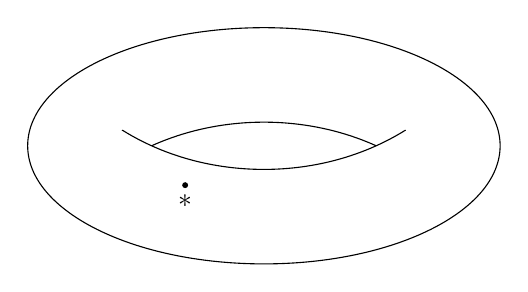
\begin{tikzpicture}
                        \useasboundingbox (-3,-1.5) rectangle (3,1.5);
                        \draw (0,0) ellipse (3 and 1.5);
                        \coordinate [label=below:$\ast$] (0) at (-1,-0.5);
                        \draw[fill] (0) circle [radius=0.03];
                        \begin{scope}
                            \clip (0,-1.8) ellipse (3 and 2.5);
                            \draw (0,2.2) ellipse (3 and 2.5);
                        \end{scope}
                        \begin{scope}
                            \clip (0,2.2) ellipse (3 and 2.5);
                            \draw (0,-2.2) ellipse (3 and 2.5);
                        \end{scope}
                \end{tikzpicture}
                \]
                \begin{align*}
                  &Y = \underset{pt}{\{*\}} \hookrightarrow X\\
                  &0 \rightarrow C_n(Y) \rightarrow C_n(X) \rightarrow C_n(X/\ast) \rightarrow 0\\
                  &H_n(Y) = \left\{ \begin{array}{cc}0&n\ne0\\\mathbb{Z}&n=0\end{array} \right. \quad \\
                  &\cdots \rightarrow H_n(Y) \rightarrow H_n(X) \rightarrow H_n(X,\ast) \rightarrow H_{n-1}(Y) \rightarrow \cdots\\
                  &\cdots \rightarrow H_0(Y) \rightarrow H_0(X) \rightarrow H_0(X,\ast) \rightarrow 0\\
                  &n > 0: \quad H_n(X,\star) = H_n(X)\\
                  &n = 0: \quad 0 \rightarrow \mathbb{Z} \rightarrow H_0(X) \rightarrow H_0(X,\ast) \rightarrow 0\\
                  &H_0(X,\star) = H_0(x)/\mathbb{Z}, \quad i.e. \left.\begin{array}{l}H_0(X) = \mathbb{Z}^d\\H_0(X) = \mathbb{Z}^{d-1}\end{array} \right.\\
                \end{align*}
               \end{Ex}

                \emph{Remark:} Sometimes one introduces ``reduced homolgy''
                \begin{align*}
                  &\dots \rightarrow C_n(X) \rightarrow C_{n-1} \rightarrow \cdots \xrightarrow{\partial_1} C_0(X) \xrightarrow{\epsilon} \mathbb{Z} \rightarrow 0, \quad \tilde{H_n}(X) \textrm{ - reduced homology}\\
                  & \sum n_i\sigma_ i \mapsto \sum_in_i \in C_0(X)\\
                  &\tilde{H_n}(X) = \left\{\begin{array}{l}H_n(X), n > 0\\H_0^{sing}(X) = H_0(X)\oplus\mathbb{Z}\end{array} \right.\\
                  & H_n(X,\ast) \rightarrow \tilde{H_n}(X)\\
                \end{align*}

              Let us consider some examples of Reduced Homology: \\

              \begin{Ex}

               Consider $X = S^1 \times [0, 1]$, and $Y = S^1 \times \{0\}$: \\

                \begin{center}


              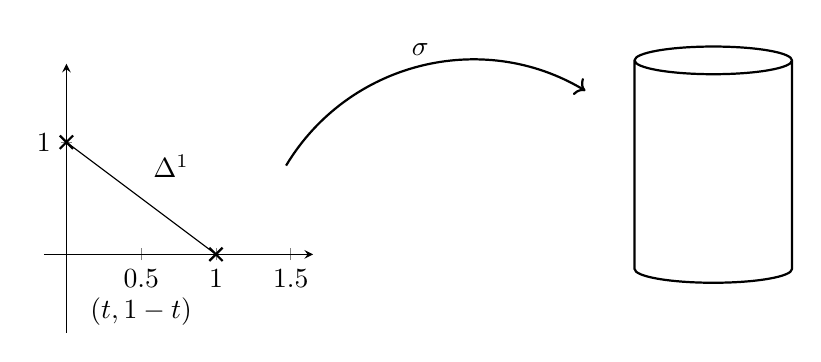
\begin{tikzpicture}
                \tikzstyle{point}=[thick,draw=black,cross out,inner sep=0pt,minimum width=4pt,minimum height=4pt]
                \begin{axis}[
                  legend pos=south west,
                  axis x line=middle,
                  axis y line=middle,
                  width=5cm,
                  height=5cm,
                  xmin=0,    % start the diagram at this x-coordinate
                  xmax=1.5,    % end   the diagram at this x-coordinate
                  ymin=-0.5,    % start the diagram at this y-coordinate
                  ymax=1.5,    % end   the diagram at this y-coordinate
                  enlargelimits=true,
                  tension=0.08]
                  \addplot[domain=0:1] {-x+1};
                  \node[point] at (axis cs:1,0) {};
                  \node[point] at (axis cs:0,1) {};
                  \node[above] at (axis cs:0.7,0.6) {$\Delta^1$};
                  \node[below] at (axis cs:0.5,-0.3) {$(t, 1-t)$};
                \end{axis}
                \draw (3,2) node (A) {};
                \draw (7,3) node (B) {};
                \draw [thick, ->] (A) to [bend left=45] node[midway, above]{$\sigma$} (B) ;

                \draw (8.5,2) node[cylinder,draw=black,thick,aspect=1.5,minimum height=3cm,minimum width=2cm,shape border rotate=90] {};
              \end{tikzpicture}

                \end{center}
                    \begin{align*}
                        &\sigma: \Delta^1 \mapsto S^1 \times [0, 1] \\
                        &\sigma: t \mapsto (\cos 2\pi t, \sin 2\pi t, 1)\\
                    \end{align*}

                The boundary operator on $\sigma$: $\partial\sigma = 0 \rightsquigarrow [\sigma] \in H_1(X)$ \\ The space $X$ is homotopic equivalent to $S^1$ so, $H_1(X) \simeq H_1(S^1) \simeq \ZZ$, considered in \ref{homotopicSpaces}. \\
              Let us take the quotient map $X/Y$. The space $Y$ will contract into a point creating a cone.

            \begin{center}

              \begin{tikzpicture}
                \tikzstyle{point}=[thick,draw=black,cross out,inner sep=0pt,minimum width=4pt,minimum height=4pt]
                \begin{axis}[
                  legend pos=south west,
                  axis x line=middle,
                  axis y line=middle,
                  width=5cm,
                  height=5cm,
                  xmin=0,    % start the diagram at this x-coordinate
                  xmax=1.5,    % end   the diagram at this x-coordinate
                  ymin=-0.5,    % start the diagram at this y-coordinate
                  ymax=1.5,    % end   the diagram at this y-coordinate
                  enlargelimits=true,
                  tension=0.08]
                  \addplot[domain=0:1] {-x+1};
                  \node[point] at (axis cs:1,0) {};
                  \node[point] at (axis cs:0,1) {};
                  \node[above] at (axis cs:0.7,0.6) {$\Delta'$};
                \end{axis}
                \draw (3,2) node (A) {};
                \draw (7,3) node (B) {};
                \draw [thick, ->] (A) to [bend left=45] node[midway, above]{$\sigma$} (B) ;

                \def\rx{1}    % horizontal radius of the ellipse
                \def\ry{0.25}  % vertical radius of the ellipse
                \def\z{1.5}     % distance from center of ellipse to origin

                \pgfmathparse{asin(\ry/\z)}
                \let\angle\pgfmathresult

                \coordinate (h) at (8.5, 1 + \z);
                \coordinate (O) at (8.5, 1);
                \coordinate (A) at ({8.5 + -\rx*cos(\angle)}, {\z-\ry*sin(\angle) + 1});
                \coordinate (B) at ({8.5 + \rx*cos(\angle)}, {\z-\ry*sin(\angle) + 1});

                \draw[fill=white!50] (A) -- (O) -- (B) -- cycle;
                \draw[fill=white!30] (h) ellipse ({\rx} and {\ry});
              \end{tikzpicture}
            \end{center}

              In $H_1(X, Y)$ the class $[\sigma] \in H_1(X)$ goes to 0 and the long exact sequence on homology is:

              \[
                H_1(Y) \rightarrow H_1(X) \rightarrow H_1(X, Y) \rightarrow H_0(X, Y) \rightarrow H_0(Y) \rightarrow H_0(X) \rightarrow 0
              \]
              where $H_1(Y), H_1(X), H_0(Y), H_0(X) \simeq \ZZ$.

             \begin{center}
              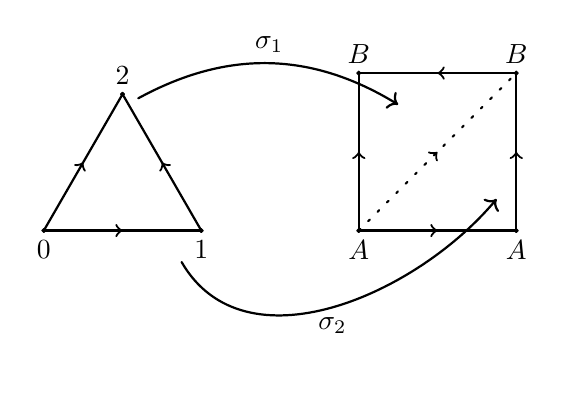
\begin{tikzpicture}[line join = round, line cap = round]

                \coordinate [label=below:$0$] (1) at (1,0);
                \coordinate [label=below:$1$] (2) at (3,0);
                \coordinate [label=above:$2$] (3) at (2,{sqrt(3)});
                \coordinate [label=above:$B$] (sb1) at (5,2);
                \coordinate [label=above:$B$] (sb2) at (7,2);
                \coordinate [label=below:$A$] (sa1) at (5,0);
                \coordinate [label=below:$A$] (sa2) at (7,0);
                \coordinate (ip1) at (2.2, 1.68);
                \coordinate (ip2) at (2.75, -0.4);
                \coordinate (ip3) at (5.5, 1.6);
                \coordinate (ip4) at (6.75, 0.4);

                \begin{scope}[decoration={markings,mark=at position 0.5 with {\arrow{to}}}]
                  \draw[fill] (1) circle [radius=0.025];
                  \draw[fill] (2) circle [radius=0.025];
                  \draw[fill] (3) circle [radius=0.025];
                  \draw[fill] (sb1) circle [radius=0.025];
                  \draw[fill] (sb2) circle [radius=0.025];
                  \draw[fill] (sa1) circle [radius=0.025];
                  \draw[fill] (sa2) circle [radius=0.025];
                  \draw[thick, postaction={decorate}] (1)--(2);
                  \draw[thick, postaction={decorate}] (1)--(3);
                  \draw[thick, postaction={decorate}] (2)--(3);
                  \draw[thick, postaction={decorate}] (sb2)--(sb1);
                  \draw[thick, postaction={decorate}] (sa1)--(sb1);
                  \draw[thick, postaction={decorate}] (sa1)--(sa2);
                  \draw[thick, postaction={decorate}] (sa2)--(sb2);
                  \draw[thick, postaction={decorate}, loosely dotted] (sa1)--(sb2);
                  \draw [thick, ->] (ip1) to [bend left=30] node[midway, above]{$\sigma_1$} (ip3) ;
                  \draw [thick, ->] (ip2) to [out=300, in=230] node[midway, below]{$\sigma_2$} (ip4) ;
                \end{scope}
              \end{tikzpicture}
             \end{center}


              \begin{align*}
               &\partial \sigma_1 = \sigma_1 |_{[12]}  - \sigma_1 |_{[02]}  + \sigma_1 |_{[01]}  \\
               &\partial \sigma_2 = \sigma_2 |_{[12]}  - \sigma_2 |_{[02]}  + \sigma_2 |_{[01]}  \\
               &\partial (\sigma_1 + \sigma_2) = \sigma_1 |_{[12]} + \sigma_2 |_{[01]}
              \end{align*}
              We can choose $\sigma = \sigma_1 |_{[12]} = \partial (\sigma_1 + \sigma_2) - \sigma_2 |_{[01]} $, $\sigma_2 |_{[01]} \in C_1(Y)$ \\
              $\sigma \in B_1(X, Y) \Rightarrow [\sigma] = 0 \in H_1(X, Y)$





              \end{Ex}

%               Notes on 4 November
%               \\
%               Gradient Ring and Module.
%               \\
%               R. Gradient ring $R = \underset{i \in \mathbb{Z}}{\oplus} R_i, \quad R_i \subseteq R$, Ab subgroups\\
%               Ex.
%               \begin{align*}
%                 &R = A[t], (A \textrm{ - commutative ring})\\
%                 &R_0 = A, R_1 = \{at, a \in A\}, \cdots, R_i = \{at', a \in A\}
%               \end{align*}
%               Ex. $R = R[x,y,z], \quad R_i = \{cx^{d_{1}}y^{d_{2}}z^{d_{3}} | \sum^3_{k=1}d_k = i\}$\\
%               Ex. $R_1 \approxeq \mathbb{R}^3$ as a vector space $\{ax + by + cz\}$\\
%               \\
%               \begin{align*}
%                 &\mathbb{N} \textrm{ - graded}, \quad \underset{i \ge 0}{\oplus}R_i, \quad M = \underset{i \in \mathbb{Z}}{\oplus} M \in R \textrm{ - mod}\\
%                 &\textrm{Graded module over } R_i, \ni M_i \subseteq M \textrm{ - ab. subgroups}\\
%                 &R_i: M_k \subseteq M_{k+1}\\
%                 &\textrm{Reminder: } R \textrm{ is a PID if it's a domain (no zero divizors)}\\
%               \end{align*}
%               Ex.
%               \begin{align*}
%                 &R = \mathbb{Z},\ or\ = (n),\ n \in \mathbb{Z}\\
%                 &R = k[1],\ b\ -\ field\\
%               \end{align*}
%               $\ast$ Check classification then for modules over PID. Thm 21. ZC and Artiin.\\
%               $\oplus D^\beta \oplus \underset{i}{\oplus} (D/d_1D)$\\
%               Graded version, $\underset{i}{\oplus} \sum^{\alpha_i}D \oplus(\underset{i}{\oplus}\sum^{\alpha_i}D/d_iD), \quad \sum^{\alpha_i}$ shift by $\alpha_i$\\
%               Ex. $D = h[t], \quad (e.g. \mathbb{R}[t])$\\
%               We can think of $D$ as module over itself\\
%               $K \oplus Kt \oplus Kt^2 \oplus \cdots$\\
%               It's also a graded module over itself\\
%               $\sum^\alpha D = t^\alpha K[t] \subseteq k[t]$, idea of $D \Rightarrow D$ - module\\
%               $M = M_\alpha \oplus M_{\alpha+1} \oplus \cdots$\\
%               $(\sum^\alpha D)_i = D_{\alpha+i}$\\
%               Comment or reduction (on the index that changes the basis): $\partial_k: \underset{\{e_i\}}{C_k} \rightarrow \underset{\{e_i^n\}}{C_{k-1}}$\\
%               $(C_{k}, C_{k1}: $ free ab groups or free R module)\\
%               \begin{align*}
%                 &\textrm{Get} M_K: \textrm{ matrix of } \partial_K. \quad e_n: {\begin{pmatrix}e_1, \cdots, e_{mk}\end{pmatrix}}{\begin{pmatrix}u_1\\\vdots\\u_{mk}\end{pmatrix}} \in C_k\\
%                 &\partial_k(eu) = \overset{n}{e}(H_u)\\
%                 &\mathcal{U}
%               \end{align*}
%               \\
%               Simplicial Complexes Combinatorically:
%               $l = \{1, 2, \cdots, m\} (=[m])$ partially ordered\\
%               Simplicial Complex is a collection $\mathcal{K}$ of subsetsof $V$\\
%               \begin{enumerate}
%               \item $\emptyset \in \mathcal{K}$
%               \item $\{i\} \in \mathcal{K}$ (simplicial)
%               \item $I \in \mathcal{K}$ and $\mathcal{J} \subseteq I \Rightarrow \mathcal{J} \in \mathcal{K}$
%               \end{enumerate}
%               $(\forall I \in \mathcal{K} (\forall J \subseteq I)) \Rightarrow \mathcal{J} \in \mathcal{K}$\\
%               Example: $\{1, 2, 3, 4\} = V$\\
%               $\mathcal{K} = \{\{1, 2, 3\} = I, \{1, 2\}, \{1, 3\}, \{2, 3\}, \{1\}, \{2\}, \{3\}, \{4\}, \emptyset\}$
%               \\
%               \\
%               \begin{tikzpicture}[line join = round, line cap = round]
%
%                 0-simplex
%                 \coordinate [label=below:$4$] (0) at (3,1.5);
%                 2-simplex
%                 \coordinate [label=below:$1$] (1) at (4,0);
%                 \coordinate [label=below:$2$] (2) at (6,0);
%                 \coordinate [label=above:$3$] (3) at (5,{sqrt(3)});
%
%                 \begin{scope}[decoration={markings,mark=at position 0.5 with
%                     {\arrow{to}}}]
%                   0-simplex
%                   \draw[fill] (0) circle [radius=0.03];
%                   2-simplex
%                   \draw[fill] (1) circle [radius=0.025];
%                   \draw[fill] (2) circle [radius=0.025];
%                   \draw[fill] (3) circle [radius=0.025];
%                   \draw[thick, postaction={decorate}] (1)--(2);
%                   \draw[thick, postaction={decorate}] (1)--(3);
%                   \draw[thick, postaction={decorate}] (2)--(3);
%                 \end{scope}
%               \end{tikzpicture}
%               \\
%               $\underset{I\in K \ne \emptyset}{\cup} (Conv(e_i)) = |\mathcal{K}|$ topology realization of $e_1, \cdots e_n \in \mathbb{R}^n$ standard basis\\
%               $X$ - top. sp\\
%               $\mathcal{U} = \{\mathcal{U}_\alpha\}_{\alpha\in A}$ - cover indexes, $\mathcal{U} = \{\mathcal{U}_1, \mathcal{U}_2, \cdots, \mathcal{U}_n\}$\\
%               $\underset{\alpha}{\cup} \quad \mathcal{U}_\alpha = X$\\
%               $\underset{"nerve\ of\ the\ cover"}{\mathcal{N}(\mathcal{U})}$: simplix of $cx$\\
%               Vertices of $\mathcal{N}(\mathcal{U}), \quad (\mathcal{N}(\mathcal{U}) = \{1, 2, \cdots, m\})$\\
%               $(k - 1)$ - faces, $\quad \{i_1, \cdots, i_k \} \in \mathcal{N}(\mathcal{U}), \quad i1 U_{1_{i}} \cap \cdots \cap \mathcal{U}_{i_{k}} \ne \emptyset$\\
%               Examples:
%               \begin{align*}
%                 &S^1 = \mathcal{U} \cup V\\
%                 &\textrm{Cover} \mathcal{U} = {U, V}\\
%               \end{align*}
%               \begin{tikzpicture}
%                 \node[circle,draw] (a) at (0,0) {};
%                 \draw[thick,-] (a) to[in=220,out=330,looseness=20] (a);
%                 \node[circle,draw] (b) at (2,-1) {};
%                 \draw[thick,-] (b) to[in=140,out=40,looseness=20] node[midway,above] {$V$} (b);
%               \end{tikzpicture}
%               \\
%               $\mathcal{U} = S' \backslash \{0, 0\}$\\
%               \begin{tikzpicture}
%                 \node[circle,draw] (a) at (0,0) {};
%                 \node[circle,draw] (b) at (0,-2) {};
%                 \draw[thick,-] (b) to[in=180,out=180] node[midway,left] {$\underset{U_1}{\mathcal{U}} \cap \underset{U_2}{V} = $} (a);
%                 \draw[thick,-] (b) to[in=0,out=0] (a);
%               \end{tikzpicture}
%               \\
%               $\{\{1, 2\}, \{1\},\{2\}, \emptyset\} = \mathcal{N}(\mathcal{U})$\\
%               Thm: (Alexandroff, ``nerve thm'') of $X$ - paracompact\\
%               $\mathcal{U} = \{\mathcal{U}_2\}$ - open cover ($\mathcal{V}_2 \subseteq X$ - open) and a good cover ($all\ \mathcal{V}_2 \&\ all\ \mathcal{V}_i \cap \cdots \cap \mathcal{V}_{i_{k}}$ are contractable or $\emptyset$)\\
%               $\underset{\underset{redirohan}{topological}}{\mathcal{N}(\mathcal{U})}$ is homotopic eq to $X$\\
%               Yes can recover $X$ by the homotopic equivalence of the nerve $(\mathcal{U})$\\


             \chapter{Persistent Homology}

                Persistent homology (PH) is a method used in topological data analysis (TDA) to study
                qualitative features of data that persist across multiple scales. Due to its construction, persistent homology computations are
                robust to perturbation of the data. Also, PH is used to extract relevant features of the data, and separate them from noise. \\

                An important result in computing persistent homology is that the persistent homology of a filtered d-dimensional simplicial
                complex is simply the standard homology of a particular graded module over a polynomial ring \cite{Zomorodian_Carlsson_2005}.\\
                Before introducing Persistent homology and understanding its calculation, we need to provide some preliminary concept from algebra.

                We begin by reviewing graded modules and rings and then stating the structure of finitely generated modules over principal
                ideal domains. Then, referring to the notions introduced in Chapter \ref{chapter1}, we provide some
                comments of the reduction algorithm used for computing simplicial homology. We conclude this chapter by describing persistent
                homology.


                \section{Background}
              \subsection{Graded Rings and Modules}

              A graded ring is a ring $\langle R, +, \cdot \rangle$ equipped with a direct sum decomposition of Abelian
              groups $R \cong \underset{i \in \mathbb{Z}}{\oplus} R_i$, so multiplication is defined by bilinear pairings $R_n \otimes R_m \rightarrow R_{n+m}$. \\

              Elements in a single $R_i$ are called homogeneous and have degree i, $\deg e = i$ for all $e \in R_i$.

              \begin{Ex}
                $ R = A[t]$, where  $(A \textrm{ - commutative ring})$
              \begin{align*}
                R_0 = A, \quad R_1 = \{at, a \in A\}, \quad \dots \ , R_i = \{at^i, a \in A\}
              \end{align*}
              \end{Ex}
              \begin{Ex}
                $R = \RR[x,y,z]$
                \[
                R_i = \{cx^{d_{1}}y^{d_{2}}z^{d_{3}} | \sum^3_{k=1}d_k = i\}\\
                \]
              For example $R_1 \simeq \mathbb{R}^3$ as a vector space $\{ax + by + cz\}$\\
              \end{Ex}

%               $\mathbb{N}$ - graded $\underset{i \ge 0}{\oplus}R_i$\\

               A graded module $M$ over a graded ring $R$ is a module equipped with a direct sum decomposition $M \cong \underset{i \in \mathbb{Z}}{\oplus} M_i$, so that the action of R on M is defined is bilinear pairings $R_n \otimes M_m \rightarrow M_{n+m}$. \\

              A graded ring (module) is non-negatively graded if $R_i = 0 \ (M_i = 0)$ for all $i < 0$.

              \emph{Note:} $R$ is a PID if it's a domain (no zero divisors) \& all its ideal are principal\\

             For example:
              \begin{align*}
                &R = \ZZ, \ I = (n),\ n \in \mathbb{Z} \\
                &R = k[t],\ k\ -\ field\\
              \end{align*}

              The structure theorem describes finitely generated modules and graded modules over PIDs.
              \begin{thm} [Structure Theorem] \label{Structure}
              If $D$ is a PID, then every finitely generated D-module is isomorphic to a direct sum of cyclic D-module. That is, it decomposes uniquely into the form
              \begin{align}
                D^\beta \oplus (\underset{i}{\oplus} D/d_iD)),
              \end{align}
              for $d_i \in D$, $\beta \in \ZZ$, such that $d_i| d_{i+1}.$ Similarly, every graded module $M$ over a graded PID D decomposes uniquely into the form
               \begin{align}
                (\underset{i}{\oplus} \Sigma^{\alpha_i} D) \oplus (\underset{i}{\oplus} \Sigma ^{\gamma_j} D/d_jD)),
              \end{align}
              where $d_j \in D$ are homogeneous elements so that $d_j|d_{j+1}$, $\alpha_i, \gamma_j in \ZZ$, and $\Sigma^\alpha$ denotes an $\alpha$-shift upward in grading.
              \end{thm}
              The free portion on the left is a vector includes generators that may generate an infinite number of elements. Decomposition (3.1) has a vector space of dimension $\beta$. The torsional portion on the right includes generators that
               may generate a finite number of elements. These torsional elements are also homogeneous. Intuitively then, the theorem describes finitely generated modules and graded modules as structures that look like vector spaces but also
                have some dimensions that are "finite" in size.


              \begin{Ex}
               Let us take $D = k[t] - \textrm{graded ring} (\textrm{e.g. } \mathbb{R}[t])$
               then:
               \[
                D = \equalto{k}{M_0} \oplus \equalto{kt}{M_1} \oplus \equalto{kt^2}{M_2} \oplus \cdots
                \]
                is also a graded module over itself.
              \begin{align*}
                &M = \sum^\alpha D = t^\alpha k[t] \subseteq k[t] \textrm{  is an ideal of } D \Rightarrow D \textrm{ - module}\\
                &M = \simequalto{M_\alpha}{k} \oplus \simequalto{M_{\alpha+1}}{kt} \oplus \cdots\\
                &(\sum^\alpha D)_i = D_{\alpha+i}\\
              \end{align*}
              \end{Ex}

              \subsection{Reduction}

              The reduction algorithm is the standard method used in computing homology. For simplicity,
              we describe the method for integer coefficients. However, the method applies also to modules over arbitrary PIDs. \\

              Given $C_k$, we can use as standard basis the oriented k-simplices:
              \begin{align*}
                &\partial_k: \underset{\{e_i\}}{C_k} \rightarrow \underset{\{\hat{e_i}\}}{C_{k-1}}\\
                &(C_{k}, C_{k-1}: \textrm{free abelian groups or free R-module})\\
                & M_k: \textrm{standard matrix representation of } \partial_k\\
                &e \cdot u: {\begin{pmatrix}e_1, \cdots, e_{m_k}\end{pmatrix}}{\begin{pmatrix}u_1\\\vdots\\u_{m_k}\end{pmatrix}} \in C_k\\
                &\partial_k(eu) = \hat{e}(M_u)\\
              \end{align*}

               The null-space of $M_k$ corresponds to $Z_k$ and its range-space to
                $B_{k?1}$. The reduction algorithm derives alternate bases for the
                chain groups, relative to which the matrix for $\partial_k$ is diagonal. The algorithm utilizes the following elementary column operations on $M_k$:

                \begin{itemize}
                 \item exchange column i, and column j,
                 \item multiply column i by -1
                 \item replace column i by (column i) + q(column j), where $q \in \ZZ$ and $i \ne j$
                \end{itemize}

                The algorithm also uses elementary row operation that are similarly defined. The idea of the reduction algorithm is to systematically modify the bases of $C_k$ and $C_{k?1}$ using elementary operations so that it reduce $M_k$ to its Smith normal form:

              Row-operation
              \begin{align*}
                &R_i \mapsto R_i + qR_j \textrm{ on } M\\
                &M \mapsto i\underbrace{\begin{pmatrix}1&&&& \\ & \ddots &&& \\ && 1 & \cdots & q \\ &&& \ddots & \\ &&&& 1 \end{pmatrix}}_\text{A} M\\
                &R_2 \mapsto R_2 + 2R_3\\
                &\begin{pmatrix}1&0&0\\0&1&2\\0&0&1\end{pmatrix} M\\
                &\begin{pmatrix}e_1 & e_2 & e_3\end{pmatrix}\begin{pmatrix}1&0&0\\0&1&2\\0&0&1\end{pmatrix} \mapsto \begin{pmatrix}e_1 & e_2 & 2e_2 + e_3\end{pmatrix}
              \end{align*}
              Column operations:
              \begin{align*}
                M \mapsto MB, B_2\begin{pmatrix}1&&&& \\ & \ddots &&& \\ && 1 && \\ && \vdots & \ddots & \\ && q && 1 \end{pmatrix}
              \end{align*}
              \\
              Interpretation of row/column operations on a matrix of a map in terms of changing bases.
              \begin{align*}
                &\partial: \xi = \underline{e}u \mapsto \hat{e} M u
                \ where\ u = [\xi]\underline{e}
              \end{align*}
              \\
              Suppose we perform a column-operation $M \mapsto MB$. This is supposed to change the matrix of a map - keeping the map unchanged
              \begin{align*}
                &\xi = \equalto{\underline{e}u}{\underline{e} B (B^{-1}u)} \mapsto \hat{e} M u = \hat{e} M B (B^{-1}u)\\
                &\textrm{If we set } \underline{e}' = \underline{e}B\\
                &\partial: \xi = \underline{e}' v \mapsto \underline{\hat{e}} MB v\\
                &v = [\xi]_{\underline{e}'}
              \end{align*}
              \\
              Similarly, suppose we perform a row-operation $M \mapsto AM$. Then
              \begin{align*}
                \xi = \underline{e}u \mapsto \underline{\hat{e}}Mu &= \underline{\hat{e}}A^{-1}AMu\\
                                                           &= \underline{\hat{e}}'AMu\\
              \end{align*}
              That is, if $M = [\partial]_{\underline{e}\underline{\hat{e}}}$, then
              \begin{align*}
                &AMB = [\partial]_{\underline{e}B, \underline{\hat{e}}A^{-1}}\\
                &A = I + qE_{ij}: R_i \mapsto R_i + qR_j \ (\textrm{via } M \mapsto AM)\\
                &A^{-1} = I - qE_{ij}\\
                &\underline{\hat{e}} A^{-1} = (\hat{e}_1, \cdots, \hat{e}_{m_{k-1}})\begin{pmatrix}1 &&&& \\ & 1 &&& \\ && \ddots & \cdots & q\\ &&& 1 &\\ &&&& 1\end{pmatrix}i =\\
                &= (\hat{e}_1, \cdots, \hat{e}_j - q\hat{e}_i, \cdots), \textrm{i.e. } \hat{e}_j \mapsto \hat{e}_j - q\hat{e}_i\\
              \end{align*}

              \begin{align*}
                &B = I + qE_{ji}: C_i \mapsto C_i + qC_j (\textrm{via } M \mapsto MB)\\
                &\underline{e}B = (e_1, \cdots, e_{m_{k}})\begin{pmatrix}1 &&&& \\ & 1 &&& \\ && \ddots & \cdots & q\\ &&& 1 &\\ &&&& 1\end{pmatrix}j = (e_1, \cdots, e_i + qe_j, \cdots)\\
              \end{align*}
              \begin{align*}
                &\textrm{Let } V \simeq \mathbb{\RR}^n (\textrm{be a vector space})\\
                &B = \{e_1, \cdots, e_n\}\\
                &V = \underline{e}X = (e_1, \cdots, e_a)\begin{pmatrix}x_1\\\vdots\\x_n\end{pmatrix}= \sum_{i=1}^nx_ie_i \quad (e_i \in V, x_i \in \mathbb{R})\\
                &B^1 = \{f_1, \cdots, f_n\}\\
                &v = \underline{e}X = \underbrace{\underline{e} T^{-1}}_\text{\underline{f}}(\underbrace{TX}_\text{Y})= (f_1, \cdots, f_n) Y\\
                &(f_1, \cdots, f_n) = (l_1, \cdots, l_n) T^{-1}\\
                &Y = TX \\
                \end{align*}
              \\
              Smith normal form (for PID):
              \begin{align*}
                &\exists A, B:\\
                &\partial_k \equiv AMB = \left(\begin{array}{c|c}
                               \begin{pmatrix}b_1 && \\ & \ddots & \\ && b_l\end{pmatrix}& \overbrace{0}^\text{}\\
                               \hline
                               0 & 0 \\
                             \end{array}\right)^{b_{i} | b_{ix1}}
                \\
                &rank Z_k = m_k - e_k\\
                &rank\ H_k = m_k - e_k - e_{k+1}
              \end{align*}
              \\





              \section{The Persistence Module}

              In this section we will combine the homology of all the complexes in the filtration
            into a single algebraic structure. We then establish a correspondence that reveals a simple
            description over fields. Most significantly, we illustrate that the persistent homology of
            a filtered complex is simply the standard homology of a particular graded module over
            a polynomial ring.

              Taking into consideration the construction of a filtered simplicial complex introduced in section \ref{complexfiltration}, we can construct a filtered chain complex: \\
              \[
                    \equalto{(0)}{C_\bullet^0} \subseteq C_\bullet^1 \subseteq C_\bullet^2 \subseteq \cdots \subseteq \equalto{C_\bullet^m}{C_\bullet}
              \]

              \begin{defn} (Persistent Homology Group). Given a filtered complex, the i-th complex $K^i$ has associated boundary operators
                $\partial^i_k$, matrices $M^i_k$ , and groups $C^i_k$, $Z^i_k$, $B^i_k$, and $H^i_k$ for all $i, k \geq 0$
                The p-persistent k-th homology group of $K^i$ is
                        \[
                        H_k^{i, p} = Z_k^i \left/ (B_k^{i+p} \cap Z_k^i) \right.
            \]
            \end{defn}

              For $p = 0$, this is the usual homology formula:
               \[ H_k(C_\bullet^i) = Z_k^i / {(B_k^i \cap Z_k^i}) = Z_k^i / B_k^i \]
             \begin{defn} (Persistence Complex)

             A persistence complex $\mathcal{C}$ is a family of chain complexes $\{C_*^i\}_{i \geq 0}$ over R, together with a chain map's $f_i: C_*^i \rightarrow C_*^{i+1}$ so that we have the following diagram:

             \[
               C_*^0 \xrightarrow{f^0} C_*^1 \xrightarrow{f^1} C_*^2 \xrightarrow{f^2} \dots
             \]


             \end{defn}

             \begin{Ex}

              Let us consider the following filtered simplicial complex, and the filtered chain complex: \\

              \begin{center}


              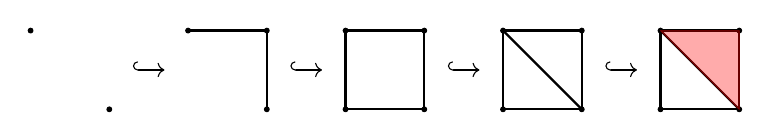
\begin{tikzpicture}[line join = round, line cap = round]
                % 1st
                \coordinate (0) at (0,1);
                \coordinate (1) at (1,0);
                % arrow 1st to 2nd
                \coordinate (a1) at (1.3, 0.5);
                \coordinate (a2) at (1.7, 0.5);
                % 2nd
                \coordinate (2) at (2,1);
                \coordinate (3) at (3,0);
                \coordinate (4) at (3,1);
                % arrow 2nd to 3rd
                \coordinate (a3) at (3.3, 0.5);
                \coordinate (a4) at (3.7, 0.5);
                % 3rd
                \coordinate (5) at (4,1);
                \coordinate (6) at (4,0);
                \coordinate (7) at (5,1);
                \coordinate (8) at (5,0);
                % arrow 3rd to 4th
                \coordinate (a5) at (5.3, 0.5);
                \coordinate (a6) at (5.7, 0.5);
                % 4th
                \coordinate (9) at (6,1);
                \coordinate (10) at (6,0);
                \coordinate (11) at (7,1);
                \coordinate (12) at (7,0);
                % arrow 4th to 5th
                \coordinate (a7) at (7.3, 0.5);
                \coordinate (a8) at (7.7, 0.5);
                % 5th
                \coordinate (13) at (8,1);
                \coordinate (14) at (8,0);
                \coordinate (15) at (9,1);
                \coordinate (16) at (9,0);

                \begin{scope}[decoration={markings,mark=at position 0.5 with {\arrow{to}}}]
                  \draw[fill] (0) circle [radius=0.03];
                  \draw[fill] (1) circle [radius=0.03];
                  \draw[fill] (2) circle [radius=0.03];
                  \draw[fill] (3) circle [radius=0.03];
                  \draw[fill] (4) circle [radius=0.03];
                  \draw[fill] (5) circle [radius=0.03];
                  \draw[fill] (6) circle [radius=0.03];
                  \draw[fill] (7) circle [radius=0.03];
                  \draw[fill] (8) circle [radius=0.03];
                  \draw[fill] (9) circle [radius=0.03];
                  \draw[fill] (10) circle [radius=0.03];
                  \draw[fill] (11) circle [radius=0.03];
                  \draw[fill] (12) circle [radius=0.03];
                  \draw[fill] (13) circle [radius=0.03];
                  \draw[fill] (14) circle [radius=0.03];
                  \draw[fill] (15) circle [radius=0.03];
                  \draw[fill] (16) circle [radius=0.03];
                  % hooks
                  \draw [right hook->] (a1) -- (a2);
                  \draw [right hook->] (a3) -- (a4);
                  \draw [right hook->] (a5) -- (a6);
                  \draw [right hook->] (a7) -- (a8);
                  % 2nd
                  \draw[thick] (3)--(4);
                  \draw[thick] (2)--(4);
                  % 3rd
                  \draw[thick] (5)--(6);
                  \draw[thick] (5)--(7);
                  \draw[thick] (6)--(8);
                  \draw[thick] (7)--(8);
                  % 4th
                  \draw[thick] (9)--(10);
                  \draw[thick] (9)--(11);
                  \draw[thick] (10)--(12);
                  \draw[thick] (11)--(12);
                  \draw[thick] (9)--(12);
                  % 5th
                  \draw[thick] (13)--(14);
                  \draw[thick] (13)--(15);
                  \draw[thick] (14)--(16);
                  \draw[thick] (15)--(16);
                  \draw[thick] (13)--(16);
                \end{scope}
                \filldraw [opacity=.33,red] (8,1) -- (9,1) -- (9,0) -- cycle;
              \end{tikzpicture}
              \end{center}

              \[
                \begin{tikzcd}[ampersand replacement=\&]
                  \& 0 \arrow[rr] \arrow[d]                      \&\& 0 \arrow[rr] \arrow[d]                                \&\& 0 \arrow[rr] \arrow[d]                            \&\& 0 \arrow[rr] \arrow[d]                            \&\& \mathbb{Z} \arrow[d]\\
                  \& 0 \arrow[hookrightarrow]{rr}{f^0} \arrow[d] \&\& \mathbb{Z}^2 \arrow[hookrightarrow]{rr}{f^2} \arrow[d] \&\& \mathbb{Z}^4 \arrow[hookrightarrow]{rr}{f^3} \arrow[d] \&\& \mathbb{Z}^5 \arrow[d] \arrow[hookrightarrow]{rr} \&\& \mathbb{Z}^4 \arrow[d]\\
                  \& \mathbb{Z}^2 \arrow[hookrightarrow]{rr}{f^0} \arrow[d] \&\& \mathbb{Z}^3 \arrow[hookrightarrow]{rr} \arrow[d] \&\& \mathbb{Z}^4 \arrow[hookrightarrow]{rr} \arrow[d] \&\& \mathbb{Z}^4 \arrow[d] \arrow[hookrightarrow]{rr} \&\& \mathbb{Z}^4 \arrow[d]\\
                  \& 0 \arrow[hookrightarrow]{rr}{f^0}           \&\& 0 \arrow[hookrightarrow]{rr}         \&\& 0 \arrow[hookrightarrow]{rr}          \&\& 0 \arrow[hookrightarrow]{rr} \&\& 0 \\
                  \& C_\bullet^0 \arrow[hookrightarrow]{rr}{f^0}       \&\& C_\bullet^1 \arrow[hookrightarrow]{rr}{f^1} \&\& C_\bullet^2 \arrow[hookrightarrow]{rr}{f^2} \&\& C_\bullet^3 \arrow[hookrightarrow]{rr}{f^3} \&\& C_\bullet^4 \\
                \end{tikzcd}
              \]
             \end{Ex}

             \begin{defn} (Persistence Module). A persistence module $\mathcal{M}$ is a family of $R-modules$, $M^i$, together
             with homomorphism $\varphi^i: M^i \rightarrow M^{i+1}\}$
             \end{defn}

             Suppose we have a persistence module  $\mathcal{M} = \{M^i, \varphi^i: M^i \rightarrow M^{i+1}\}$ over a
             ring $R$, We can equip $R[t]$ with the standard grading and define a graded module over $R[t]$ by
                \[ \alpha(M) = \underset{i \ge 0}{\oplus} M_i \],
                where the $R-module$ structure is the sum of the structures on the individual components, and where the action of t is given by:

              \begin{align*}
                &t \cdot(m^0,m^1, \cdots) = (0, \varphi^0(m^0), \varphi^1(m^1), \cdots)\\
                &\left(\begin{array}{c|c|c|c}
                        0 &&& \\ \hline \varphi^0 & 0 && \\ \hline & \varphi^1 & 0 & \\ \hline && \varphi^2 &
                      \end{array}\right)
              \end{align*}

              $t$ simply shift elements of the module up in gradation.

            \begin{Ex}

              \begin{align*}
                &\varphi: \mathbb{R}^n \rightarrow \mathbb{R}\\
                &\varphi: \begin{pmatrix}x_1\\\vdots\\x_n\end{pmatrix} \mapsto (A_1, \cdots, A_n)\begin{pmatrix}x_1\\\vdots\\x_n\end{pmatrix} = A_1x_1 + \cdots + A_nx_n\\
                &(\varphi_1, \cdots, \varphi_{n-1}) \mathbb{R}^n \rightarrow \mathbb{R}^{n-1}\\
                &\underline{x} \mapsto \begin{pmatrix}A_{11} & \cdots & A_{m-1}\\ \cdots&\cdots&\cdots\end{pmatrix}\begin{pmatrix}x_1\\\vdots\\x_n\end{pmatrix}\\
                &\textrm{e.g.} \begin{pmatrix}1&0&0\\0&1&0\end{pmatrix}:\begin{pmatrix}x\\y\\z\end{pmatrix} \mapsto \begin{pmatrix}x\\y\end{pmatrix}\\
              \end{align*}

            \end{Ex}


              \begin{thm} (Correspondence) The correspondence $\alpha$ defines an equivalence of categories between the category of persistence modules of finite type over $R$ and the category of finitely generated non-negatively graded modules over $R[t]$.
              \end{thm}

            The Correspondence theorem gives us a simple decomposition when the ground ring is a field $F$. In this case the graded ring $F[t]$ is a PID and its only graded ideals are homogeneous of form $(t_n)$, so the structure of the $F[t]-module$ is described by sum (3.2) in structure theorem \ref{Structure}:

            \begin{align}
                (\underset{i}{\oplus} \Sigma^{\alpha_i} F[t]) \oplus (\underset{j}{\oplus} \Sigma ^{\gamma_j} F[t]/(t^{n^j})).
              \end{align}
              
              
              
              \section{\v{C}ech and Vietoris-Rips Complex}
              \label{CechRips}
              
              In a ever-increasing world of data, the need for data analysis techniques and method is very high. 
              Topological Data Analysis is a relatively new sphere in Data Analysis, that is bringing new insights in the study of data. 
              
              The principal themes is previous surveys from Carlsson, de Silva, Harer, Zomorodian and other, are:
              \begin{enumerate}
               \item It is useful to replace a set of data points with a family of simplicial complexes, indexed by a 
               procimity parameter. 
               \item It is beneficial to use persistent homology to calculate these topological complexes.
               \item It is helpful to encode the persistent homology of a data set in the form
of a parameterized version of a Betti number: a barcode
              \end{enumerate}
              
              Data is collected from different number of sources, and comes in a variety of form and shapes. Often data is represented as a unordered sequence of points in a Euclidean $n-dimentional$ space $\mathbb{E}^n$. The overall shape of data might provide important information about the underlying phenomena that
              the data repesents. A \textbf{point cloud data} is the type of dataset where global feature are present and important. It is exaclty this type of data that is tackled by persistent homology. \cite{Ghrist_2007}
              
              Naturally, the question of how to represent a collection of points $\{x_\alpha\}$, rises. 
              A straightforward approach would be to use the point cloud as vertices of a combinatorial graph whose
              edges are determined by proximity, for example within a specific distance $\epsilon$. A graph of this type can capture the connection of the point cloud,
              but it will fail to detect any higher order features beyond clustering. 
              A good way to tackle this issue, it to complete the graph to a simplicial complex. The choice of how to fill in the higher dimensional simplices of the proximity graph will result in different global representaions. 
              
              Two more prominant ways on how to fill in the higher dimensional simplices are:  \v{C}ech and Vietoris-Rips Complex: 
              
              \begin{defn} \label{cech} (\v{C}ech Complex)
           Given a collection of points $\{x_\alpha\}$ in Euclidean space $\mathbb{E}^n$, the \v{C}ech Complex, $\mathcal{C}_\epsilon$, is the abstract simplicial complex whose k-simplices are determined by unordered (k+1)-uple of points $\{x_\alpha\}_0^k$ whose closed $\epsilon/2-ball$ neighborhoods have a point of common intersection. 
              \end{defn}
           

            For example: 
             \begin{center}
              


            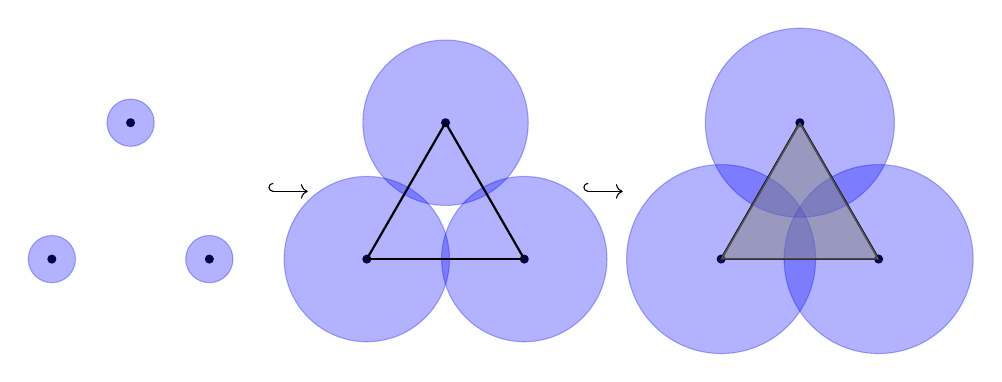
\begin{tikzpicture}[line join = round, line cap = round]

                        % first-simplex
                        \coordinate (0) at (0,0);
                        \coordinate (1) at (2,0);
                        \coordinate (2) at (1,{sqrt(3)});
                       
                         % second-simplex
                        \coordinate  (3) at (4,0);
                        \coordinate  (4) at (6,0);
                        \coordinate  (5) at (5,{sqrt(3)});
                        
                        % third-simpex
                        \coordinate  (6) at (8.5,0);
                        \coordinate  (7) at (10.5,0);
                        \coordinate  (8) at (9.5,{sqrt(3)});

                        \begin{scope}[decoration={markings,mark=at position 0.5 with
                            {\arrow{to}}}]
                            
                            % first-simplex
                            \draw[fill] (0) circle [radius=0.05];
                            \draw[fill, opacity=0.3, blue] (0) circle [radius=0.3];
                            \draw[fill] (1) circle [radius=0.05];
                            \draw[fill, opacity=0.3, blue] (1) circle [radius=0.3];
                            \draw[fill] (2) circle [radius=0.05];
                            \draw[fill, opacity=0.3, blue] (2) circle [radius=0.3];
                            \draw [thin, right hook->] (2.75, 0.86) -- (3.25, 0.86);  
                            
                            % second-simplex
                            \draw[fill] (3) circle [radius=0.05];
                            \draw[fill, opacity=0.3, blue] (3) circle [radius=1.05];
                            \draw[fill] (4) circle [radius=0.05];
                            \draw[fill, opacity=0.3, blue] (4) circle [radius=1.05];
                            \draw[fill] (5) circle [radius=0.05];
                            \draw[fill, opacity=0.3, blue] (5) circle [radius=1.05];
                            \draw[thick] (3)--(4);
                            \draw[thick] (3)--(5);
                            \draw[thick] (4)--(5);
                            \draw [thin, right hook->] (6.75, 0.86) -- (7.25, 0.86);  
            
                            
                           % third-simpex
                            \draw[fill] (6) circle [radius=0.05];
                            \draw[fill, opacity=0.3, blue] (6) circle [radius=1.2];
                            \draw[fill] (7) circle [radius=0.05];
                            \draw[fill, opacity=0.3, blue] (7) circle [radius=1.2];
                            \draw[fill] (8) circle [radius=0.05];
                            \draw[fill, opacity=0.3, blue] (8) circle [radius=1.2];
                            \draw[thick] (6)--(7);
                            \draw[thick] (6)--(8);
                            \draw[thick] (7)--(8);
                            \filldraw[opacity=.5, gray] (6) --  (7) --  (8) -- cycle;
                        \end{scope}

                    \end{tikzpicture} 
                    

             \end{center}

           \begin{defn} (Vietoris-Rips Complex) \label{rips}
              Given a collection of points $\{x_\alpha\}$ in Euclidean space $\mathbb{E}^n$, the Rips Complex, $\mathcal{R}_\epsilon$, is the abstract simplicial complex whose k-simplices correspond to unordered (k+1)-uple of points $\{x_\alpha\}_0^k$ which are pairwise within distance $\epsilon$. 
            \end{defn}
            
            For example: 
            \begin{center}
             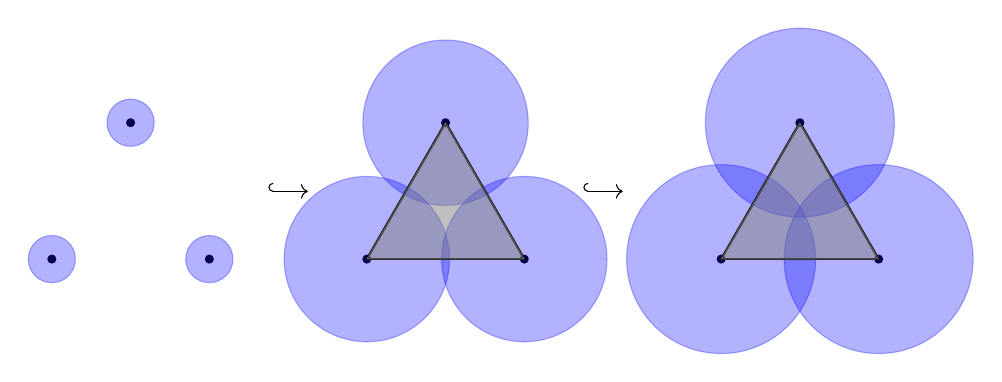
\begin{tikzpicture}[line join = round, line cap = round]

                       % first-simplex
                        \coordinate (0) at (0,0);
                        \coordinate (1) at (2,0);
                        \coordinate (2) at (1,{sqrt(3)});
                       
                         % second-simplex
                        \coordinate  (3) at (4,0);
                        \coordinate  (4) at (6,0);
                        \coordinate  (5) at (5,{sqrt(3)});
                        
                        % third-simpex
                        \coordinate  (6) at (8.5,0);
                        \coordinate  (7) at (10.5,0);
                        \coordinate  (8) at (9.5,{sqrt(3)});

                        \begin{scope}[decoration={markings,mark=at position 0.5 with
                            {\arrow{to}}}]
                            % first-simplex
                            \draw[fill] (0) circle [radius=0.05];
                            \draw[fill, opacity=0.3, blue] (0) circle [radius=0.3];
                            \draw[fill] (1) circle [radius=0.05];
                            \draw[fill, opacity=0.3, blue] (1) circle [radius=0.3];
                            \draw[fill] (2) circle [radius=0.05];
                            \draw[fill, opacity=0.3, blue] (2) circle [radius=0.3];
                            \draw [thin, right hook->] (2.75, 0.86) -- (3.25, 0.86);  
                            % second-simplex
                            \draw[fill] (3) circle [radius=0.05];
                            \draw[fill, opacity=0.3, blue] (3) circle [radius=1.05];
                            \draw[fill] (4) circle [radius=0.05];
                            \draw[fill, opacity=0.3, blue] (4) circle [radius=1.05];
                            \draw[fill] (5) circle [radius=0.05];
                            \draw[fill, opacity=0.3, blue] (5) circle [radius=1.05];

                            \draw[thick] (3)--(4);
                            \draw[thick] (3)--(5);
                            \draw[thick] (4)--(5);
                           \draw [thin, right hook->] (6.75, 0.86) -- (7.25, 0.86);  
                            \filldraw[opacity=.5, gray] (3) --  (4) --  (5) -- cycle;
                           % third-simpex
                            \draw[fill] (6) circle [radius=0.05];
                            \draw[fill, opacity=0.3, blue] (6) circle [radius=1.2];
                            \draw[fill] (7) circle [radius=0.05];
                            \draw[fill, opacity=0.3, blue] (7) circle [radius=1.2];
                            \draw[fill] (8) circle [radius=0.05];
                            \draw[fill, opacity=0.3, blue] (8) circle [radius=1.2];
                            \draw[thick] (6)--(7);
                            \draw[thick] (6)--(8);
                            \draw[thick] (7)--(8);
                            \filldraw[opacity=.5, gray] (6) --  (7) --  (8) -- cycle;
                        \end{scope}

                    \end{tikzpicture} 
            \end{center}
            
             If $X$ is a topological space, and $X = \underset{\alpha}{\cup} \quad \mathcal{U}_\alpha$ 
             where $\mathcal{U} = \{\mathcal{U}_\alpha\}_{\alpha\in A}$ are cover indexes, $\mathcal{U} = \{\mathcal{U}_1, \mathcal{U}_2, \cdots, \mathcal{U}_n\}$, given a cover $\mathcal{U}$ (not necessarily open) of a space $X$, the nerve of $\mathcal{U}$ is a simplicial complex  $\mathcal{N}(\mathcal{U})$ whose n-simplices consist of sets of $n+1$ elements of $\mathcal{U}$ with non-empty intersections.
              Vertices of $\mathcal{N}(\mathcal{U})= \{1, 2, \cdots, m\}$ are 
              $(k - 1)$ - faces if $\ \mathcal{U}_{i_{1}} \cap \cdots \cap \mathcal{U}_{i_{k}} 
              \ne \emptyset$ for $ \{i_1, \cdots, i_k \} \in \mathcal{N}(\mathcal{U})$\\
              
              \begin{Ex} Let's break the circle $S^1$ into the following spaces $U, V$: \\
              \begin{center}
              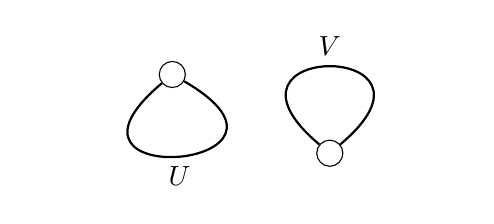
\begin{tikzpicture}
                \node[circle,draw] (a) at (0,0) {};
                \draw[thick,-] (a) to[in=220,out=330,looseness=20] node[midway,below] {$U$}(a);
                \node[circle,draw] (b) at (2,-1) {};
                \draw[thick,-] (b) to[in=140,out=40,looseness=20] node[midway,above] {$V$} (b);
                
              \end{tikzpicture}
            \end{center}
               \begin{align*}
                &S^1 = \mathcal{U} \cup V\\
                &\textrm{The cover } \mathcal{U} = \{U, V\}\\
              \end{align*}
              \\
%               $\mathcal{U} = S' \backslash \{0, 0\}$\\
                \begin{center}
 

              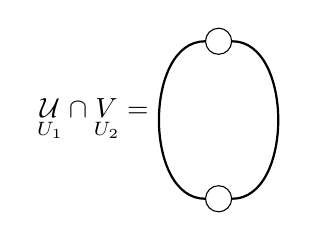
\begin{tikzpicture}
                \node[circle,draw] (a) at (0,0) {};
                \node[circle,draw] (b) at (0,-2) {};
                \draw[thick,-] (b) to[in=180,out=180] node[midway,left] {$\underset{U_1}{\mathcal{U}} \cap \underset{U_2}{V} = $} (a);
                \draw[thick,-] (b) to[in=0,out=0] (a);
              \end{tikzpicture}
                \end{center}
              
              \[
              \{\{1, 2\}, \{1\},\{2\}, \emptyset\} = \mathcal{N}(\mathcal{U})
              \]
              \end{Ex}

              
              The $\check{C}$ech complex $\mathcal{C}_\epsilon$ is the nerve of the collection of closed discs of radius $\epsilon/2$ around the points of the cloud, thought of as a cover of its union.
              \begin{thm}(The Nerve Theorem)
              
            If $X$ is a paracompact space, and $U$ is an open cover of $X$ such that the
            intersection of any finite subfamily of $U$ is either empty or contractible,
            then the realization of the nerve of $U$ is homotopy equivalent to X.\cite{hatcher}
            
              \end{thm}

    

%             \begin{align*}
%                 \xymatrix{
%                 X
%                 \\
%                 & V \amalg U \ar@<0ex>[ul]|-{!}
%                 & V \ar@/_/[ull]_{i_{v}} \ar@{_{(}->}[l]
%                 \\
%                 & U \ar@/^/[uul]^{i_{u}} \ar@{_{(}->}[u]
%                 & U \cap V \ar@{_{(}->}[l] \ar@{_{(}->}[u]
%                   }
%               \end{align*}
% 
%               \begin{align*}
%                 \xymatrix{
%                 H_n(X)
%                 \\
%                 & H_n(V) \oplus H_n(U) \ar@<0ex>[ul]
%                 & H_n(V) \ar@/_/[ull] \ar[l]
%                 \\
%                 & H_n(U) \ar@/^/[uul] \ar[u]
%                 & H_n(U \cap V) \ar[l] \ar[u]
%                   }
%               \end{align*}
%               \\
%               $X$ - topological spaces, $X = \cup_i \mathcal{U}_i$\\
%               Say $\{i_0, \cdots, i_k\}$ form a $k$ - simplex, $\mathcal{U}_{i_{m}} \cap \mathcal{U}_{i_{n}} \ne \emptyset, \quad \forall i_m, i_n \in \{i_0, \cdots, i_k\}$\\
%               Variants:\\
%               1) $x$  - metric space $\{B_{\epsilon}(p), p\in x\}$, $VR_\epsilon(x)$\\
%               2) $x$ - finite metric space. $x = \{p_1, \cdots, p_N\}$, $x \le \mathbb{R}^N$\\
%               $[p_{i_{0}}, \cdots, p_{i_{k}}]$ is a $k$ - simplex, when $dist(p_{i_{j_{1}}}, p_{i_{j_{2}}}) \le 2 \epsilon$\\
%               $\check{C}_\epsilon\cdot(x) \hookrightarrow VR_\epsilon\cdot(x) \hookrightarrow \check{C}_{2\epsilon}\cdot(x)$ improved to $\sqrt{2}$\\
%               Good news:\\
%               Both $cxs$ (complexes) are functorial in $\epsilon$ \& $x$. If $\epsilon_1 < \epsilon_2$ we get simplical map $VR_{\epsilon_{1}}\cdot (x) \rightarrow VR_{\epsilon_{2}}(x)$\\
%               ie $VR(x) \cdot R \rightarrow $ simplicial\\
%               If $f: x\rightarrow y$ Lipschitz with constant k\\
%               $d(f(p), f(q)) < kd(p,q), \quad \forall p,q \in x$\\
%               $VR_\epsilon(x) \rightarrow VR_{k\epsilon}(y)$
%               \\
%               Compose with $H_n$\\
%               $H_n(VR_{(-)}(x)): R \rightarrow Ab$\\
%               $H_n(VR_\epsilon(-)):$ {finite metric space} $\rightarrow$ Al\\
%               \\
%               Have finite set $\epsilon_1 < \epsilon_2 < \cdots$ where $H_n$ "jumps"\\
%               ie
%               \begin{align*}
%                 H_n(VR_\epsilon(x)) = \left\{\begin{array}{cc}G_1& \epsilon\in[0, \epsilon)\\G_2& \epsilon\in[\epsilon_1, \epsilon_2)\end{array}\right.
%               \end{align*}
%               \\
%               Get maps $VR_{\epsilon_{1}}(x) \rightarrow VR_{\epsilon_{2}}(x) \rightarrow H_n(VR_{\epsilon_{1}}(x)) \rightarrow H_n(VR_{\epsilon_{2}}(x))$\\
%               \\



              
              
              
            \chapter{Computing Persistent Homology}

            So far we have build the following setup to compute persistence homology on persistence chain complex:
              \begin{align*}
                &Persistence \ complex: C_\bullet^0 \hookrightarrow C_\bullet^1 \hookrightarrow C_\bullet^2 \hookrightarrow \cdots\\
                &Persistent \ Homology \ Group: \ H_k^{i,p} = Z_k^i / B_k^{i+p} \cap Z_k^i\\
                & where \ Z_k^i = \ker (\partial_k^i : C_k^i \rightarrow C_{k-1}^i)
                =\Ima ((H_k^i = H_k ( C_\bullet^i) \rightarrow (H_k ( C_\bullet^{i+p}))\\
              \end{align*}
              \section*{Remarks on Computing Persistent Homology}
              
              \begin{itemize}
               \item 

              
              Any ideal $\omega \subseteq R$ in a commutative ring in as R - module in a natural way: $\forall a \in \omega, \forall r \in R, r\cdot a \in \omega$ and $\omega \subseteq R$ is an ab\. group\. (R is a module over itself \& $\omega$ is a submodule)\\
              Hence, for any
              \begin{align*}
                n \in \mathbb{N}\\
                \equalto{(t^n)}{\{\equalto{t^n}{t^nk[t]} P(t), P \in k[t]\}} \subseteq k[t]
              \end{align*}
              is a $k[t]$ - module. This is a free $k[t]$ - module.\\
              \item 
              $R = k[t]$ has a natural structure of \underline{graded ring}. The deg $i$ - elements are the (non-zero) elements of the line $R_i := kt^i \subseteq k[t]$ (in general: $R = \oplus R_i, R_iR_j \subseteq R_{i+j}$).
              The ideal $(t^n) \subseteq k[t]$ is then a graded $k[t]$ - module (in general, this means $M = \underset{i}{\oplus} M_j, R = \underset{i}{\oplus} R_i, R_i \cdot M_j \subseteq M_{i+j}$) $(t^n) = t^n, k[t] = \underset{i \ge 0}{\oplus} \underbrace{kt^{n+i}}_{(t^{n})}$\\
              i.e.\\
              degree - i elements of $(t^n)$ are the monomials of degree $(n+i)$\\
              \item 
              While $(t^n) \subseteq k[t]$ is an ideal, so $k[t]$ - module - and so $k[t]$ - submodule; and a graded $k[t]$ - module, it is \underline{not} a graded $k[t]$ - submodule!\\
              \item
              The grading of $(t^n)$ is \underline{not} the grading that is induced by the \underline{ambient} $k[t]$: it is \underline{shifted up} by $n$: $t^{n+i}$, as an alternative of $(t^n) = t^nk[t]$, has degree $i$, not degree $(n+i)$.\\
              \item 
              In general, for a graded module $M$ over a graded ring $R$ we can define the \underline{twist of $M$ by $n$}, $M[n]$, also denoted by $\sum^nM$, is defined by $(\sum^nM)_i = M_{n+i}$.\\
              i.e., by redefining/shifting the grading up by $n$. We see that we can identify $\sum^nk[t]$ with $(t^n) = t^nk[t]$ as \underline{graded modules} $(\sum^nk[t])_i = k[t]_{n+i} = kt^{n+i} \xrightarrow{id} kt^n\cdot t^i$\\
              \item
              A map of free $k[t]$ - modules $k[t] \rightarrow k[t]$ is multiplication by some polynomial $p(t)$ ie of the kind $p(t) \mapsto p(t)q(t)$ ($p(t)$ is the image of $1 \in k[k]$). More generally, a map of free $k[t]$ - module, $k[t]^{\oplus m} \rightarrow k[t]^{\oplus r}$ is given by some $r \times m$ matrix with $k[t]$ - entries.\\
              \item
              A map (morphism) if \underline{graded R-modules} $\varphi: M \rightarrow N$ is a map of R - modules (ie: R - linear, ie: $\varphi(rm) = r \varphi(m), \varphi(m_1 + m_2) = \varphi(m_1) + \varphi(m_2)$) which \underline{preserves the degrees}. That is $\varphi(M_i) \subseteq N_i, \forall i$.\\
              In particular, a map of graded modules $\varphi: \sum^n\simequalto{k[t]}{(t^n)} \rightarrow \sum^p\simequalto{k[t]}{(t^p)}$ must send $(t^n)_i = kt^{n+i}$ to $(t^p)_i = kt^{p+i}$.\\
              \item
              As the shifts $\sum^nk[t]$ are still free modules, any $k[t]$ - module homomorphism $\varphi: (t^n) \rightarrow (t^n)$ is determined by some polynomial $p(t) \in k[t]$, ie by the image of a generator: $\varphi(t^n) = p(t)t^p$ as $\varphi(t^nq(t)) = q(t)\varphi(t^n)$. \underline{However} if $\varphi$ is a \underline{graded} module homomorphism, we must have that $\varphi(t^n) = \underbrace{(mt^p)}_{p(t)}t^p$, ie, that $p(t)$ be homogeneous. Similarly, for direct sums $\underset{i}{\oplus}(t^{ni}) \rightarrow \underset{i}{\oplus}(t^{pj})$.\\
              \item
              \underline{In particular:} if $n \ge p$, any map of modules $\varphi: k[t] \rightarrow k[t], 1 \mapsto p(t)$ determines a map of \underline{graded} modules
              \begin{align*}
                &(t^n) = \sum^nk[t] \rightarrow (t^p) = \sum^pk[t]\\
                &t^n \mapsto (p(t)t^{n-p})t^p
              \end{align*}
              \\
              E.g, the identity map on $k[t]$ induces $t^n \mapsto t^{n-p} \cdot t^p$ (The "matrix element" of the identity on $k[t]$ is $t^{n-p}$).
              \end{itemize}

              \begin{Ex} Consider $X$ to be a space consisting of two points and $Y$, of an edge.
              Then we can construct the following persistence complex: \\

              \begin{center}
                \begin{tikzpicture}[line join = round, line cap = round]
                  \coordinate (0) at (0,0);
                  \coordinate (1) at (1,0);
                  \coordinate (2) at (3,0);
                  \coordinate (3) at (4,0);
                  \begin{scope}[decoration={markings,mark=at position 0.5 with {\arrow{to}}}]
                    \draw[fill] (0) circle [radius=0.03];
                    \draw[fill] (1) circle [radius=0.03];
                    \draw[fill] (2) circle [radius=0.03];
                    \draw[fill] (3) circle [radius=0.03];
                    \draw[thick] (2)--(3);
                  \end{scope}
                \end{tikzpicture}
              \end{center}
              \begin{align*}
                \\
                \begin{tikzcd}[ampersand replacement=\&, sep=large]
                  \& C_\bullet^0 \arrow[hookrightarrow]{rr}{f_0} \&\& C_\bullet^1 \\
                  1 \& (0) \arrow[hookrightarrow]{rr} \arrow[d,swap,"\partial_1=0"]          \&\& \mathbb{Z} \arrow[d,"\partial_1={\begin{bmatrix}-1\\1\end{bmatrix}}"]\\
                  0 \& \mathbb{Z}^2 \arrow[hookrightarrow]{rr} \arrow[d,swap,"\partial_0=0"] \&\& \mathbb{Z}^2 \arrow[d,"\partial_0={\begin{bmatrix}0&0\end{bmatrix}}"]\\
                  \& 0 \arrow[hookrightarrow]{rr}              \&\& 0\\
                \end{tikzcd}
              \end{align*}
              \\
              \underline{$p = 0$}
              \begin{align*}
                &H_k^{i,0} = Z_k^i / B_k^i \cap Z_k^i\\
                &H_1^{0,0} = (0) \quad H_1^{1,0} = (0)\\
                &H_0^{0,0} = \mathbb{Z}^2 \quad H_0^{1,0} \simeq \mathbb{Z}\\
              \end{align*}
              \\
              \underline{$p = 1$}
              \begin{align*}
                &H_k^{i,1} = Z_k^i / B_k^{i+1} \cap Z_k^i\\
                &H_1^{0,1} = Z_0^1 / B_1^{1} \cap Z_1^0 = (0) \quad H_1^{1,1} = (0)\\
                &H_0^{0,1} = Z_0^0 / B_0^{1} \cap Z_0^0 = \mathbb{Z}^2 / \Ima \begin{bmatrix}-1\\1\end{bmatrix} \simeq \mathbb{Z}\\
              \end{align*}
              
              \begin{center}
              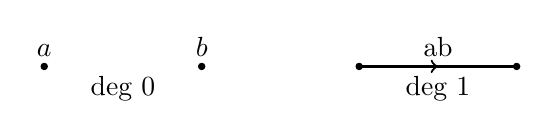
\begin{tikzpicture}[line join = round, line cap = round]
                \coordinate [label=above:$a$] (a) at (0,0);
                \coordinate [label=above:$b$] (b) at (2,0);
                \coordinate (c) at (4,0);
                \coordinate (d) at (6,0);
                \begin{scope}[decoration={markings,mark=at position 0.5 with {\arrow{to}}}]
                  \draw[fill] (a) circle [radius=0.04];
                  \draw[fill] (d) circle [radius=0.04];
                  \draw[fill] (b) circle [radius=0.04];
                  \draw[fill] (c) circle [radius=0.04];
                  \draw[draw=none] (a)--(b) node[midway,below] {deg 0};
                  \draw[thick, postaction={decorate}] (c)--(d) node[midway,above] {ab} node[midway,below] {deg 1};
                \end{scope}
              \end{tikzpicture}
              \end{center}
              
              The final complex is $0 \rightarrow \mathbb{Z} \xrightarrow{\partial_1} \mathbb{Z}^{\oplus2} \rightarrow 0$. The matrix of $\partial_1$ is \begin{align*}M_1 = \begin{bmatrix}-1\\1\end{bmatrix}.\end{align*}
              This gives rise to the complexes of $\mathbb{Z}[t] - modules$.\\
              \begin{align*}
                0 \rightarrow \mathbb{Z}[t] \xrightarrow{\begin{bmatrix}-1\\1\end{bmatrix}} \mathbb{Z}t^{\oplus2} \rightarrow 0
              \end{align*}
              and of \underline{graded} $\mathbb{Z}[t]$ -modules.
              \begin{align*}
                0 \rightarrow \mathbb{Z}[t] \xrightarrow{\begin{bmatrix}-t\\t\end{bmatrix}} \equalto{(1)^{\oplus2}}{\mathbb{Z}t^{\oplus2}} \rightarrow 0
              \end{align*}

              \end{Ex}

              \begin{Ex}
               Let us consider the following filtered complex: \\

              \begin{center}


              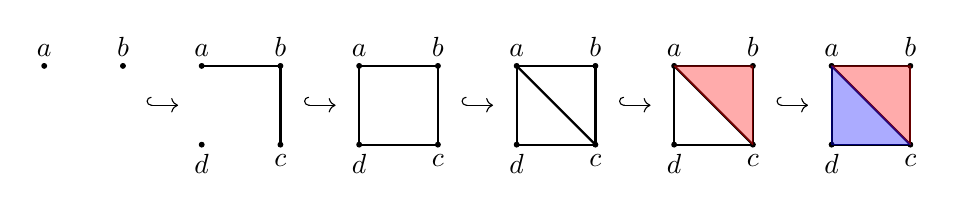
\begin{tikzpicture}[line join = round, line cap = round]
                % 1st
                \coordinate [label=above:$a$] (0) at (0,1);
                \coordinate [label=above:$b$] (1) at (1,1);
                % arrow 1st to 2nd
                \coordinate (a1) at (1.3, 0.5);
                \coordinate (a2) at (1.7, 0.5);
                % 2nd
                \coordinate [label=above:$a$] (2) at (2,1);
                \coordinate [label=below:$d$] (3) at (2,0);
                \coordinate [label=above:$b$] (4) at (3,1);
                \coordinate [label=below:$c$] (5) at (3,0);
                % arrow 2nd to 3rd
                \coordinate (a3) at (3.3, 0.5);
                \coordinate (a4) at (3.7, 0.5);
                % 3rd
                \coordinate [label=above:$a$] (6) at (4,1);
                \coordinate [label=below:$d$] (7) at (4,0);
                \coordinate [label=above:$b$] (8) at (5,1);
                \coordinate [label=below:$c$] (9) at (5,0);
                % arrow 3rd to 4th
                \coordinate (a5) at (5.3, 0.5);
                \coordinate (a6) at (5.7, 0.5);
                % 4th
                \coordinate [label=above:$a$] (10) at (6,1);
                \coordinate [label=below:$d$] (11) at (6,0);
                \coordinate [label=above:$b$] (12) at (7,1);
                \coordinate [label=below:$c$] (13) at (7,0);
                % arrow 4th to 5th
                \coordinate (a7) at (7.3, 0.5);
                \coordinate (a8) at (7.7, 0.5);
                % 5th
                \coordinate [label=above:$a$] (14) at (8,1);
                \coordinate [label=below:$d$] (15) at (8,0);
                \coordinate [label=above:$b$] (16) at (9,1);
                \coordinate [label=below:$c$] (17) at (9,0);
                % arrow 5th to 6th
                \coordinate (a9) at (9.3, 0.5);
                \coordinate (a10) at (9.7, 0.5);
                % 6th
                \coordinate [label=above:$a$] (18) at (10,1);
                \coordinate [label=below:$d$] (19) at (10,0);
                \coordinate [label=above:$b$] (20) at (11,1);
                \coordinate [label=below:$c$] (21) at (11,0);

                \begin{scope}[decoration={markings,mark=at position 0.5 with {\arrow{to}}}]
                  \draw[fill] (0) circle [radius=0.03];
                  \draw[fill] (1) circle [radius=0.03];
                  \draw[fill] (2) circle [radius=0.03];
                  \draw[fill] (3) circle [radius=0.03];
                  \draw[fill] (4) circle [radius=0.03];
                  \draw[fill] (5) circle [radius=0.03];
                  \draw[fill] (6) circle [radius=0.03];
                  \draw[fill] (7) circle [radius=0.03];
                  \draw[fill] (8) circle [radius=0.03];
                  \draw[fill] (9) circle [radius=0.03];
                  \draw[fill] (10) circle [radius=0.03];
                  \draw[fill] (11) circle [radius=0.03];
                  \draw[fill] (12) circle [radius=0.03];
                  \draw[fill] (13) circle [radius=0.03];
                  \draw[fill] (14) circle [radius=0.03];
                  \draw[fill] (15) circle [radius=0.03];
                  \draw[fill] (16) circle [radius=0.03];
                  \draw[fill] (17) circle [radius=0.03];
                  \draw[fill] (18) circle [radius=0.03];
                  \draw[fill] (19) circle [radius=0.03];
                  \draw[fill] (20) circle [radius=0.03];
                  \draw[fill] (21) circle [radius=0.03];
                  % hooks
                  \draw [right hook->] (a1) -- (a2);
                  \draw [right hook->] (a3) -- (a4);
                  \draw [right hook->] (a5) -- (a6);
                  \draw [right hook->] (a7) -- (a8);
                  \draw [right hook->] (a9) -- (a10);
                  % 2nd
                  \draw[thick] (5)--(4);
                  \draw[thick] (2)--(4);
                  % 3rd
                  \draw[thick] (6)--(7);
                  \draw[thick] (6)--(8);
                  \draw[thick] (7)--(9);
                  \draw[thick] (8)--(9);
                  % 4th
                  \draw[thick] (10)--(11);
                  \draw[thick] (10)--(12);
                  \draw[thick] (11)--(13);
                  \draw[thick] (12)--(13);
                  \draw[thick] (10)--(13);
                  % 5th
                  \draw[thick] (14)--(15);
                  \draw[thick] (14)--(16);
                  \draw[thick] (15)--(17);
                  \draw[thick] (16)--(17);
                  \draw[thick] (14)--(17);
                  % 6th
                  \draw[thick] (18)--(19);
                  \draw[thick] (18)--(20);
                  \draw[thick] (19)--(21);
                  \draw[thick] (20)--(21);
                  \draw[thick] (18)--(21);
                \end{scope}
                \filldraw [opacity=.33,red] (8,1) -- (9,1) -- (9,0) -- cycle;
                \filldraw [opacity=.33,red] (10,1) -- (11,1) -- (11,0) -- cycle;
                \filldraw [opacity=.33,blue] (10,1) -- (10,0) -- (11,0) -- cycle;
              \end{tikzpicture}
              \end{center}

              \[
                \begin{tikzcd}[ampersand replacement=\&, sep=normal]
                  \& 0     \&\& 1    \&\& 2     \&\& 3     \&\& 4     \&\& 5\\
                  \& C_\bullet^0 \arrow[rr] \&\& C_\bullet^1 \arrow[rr] \&\& C_\bullet^2 \arrow[rr] \&\& C_\bullet^3 \arrow[rr] \&\& C_\bullet^4 \arrow[rr] \&\& C_\bullet^5\\
                  2 \& 0 \arrow[d]  \arrow[rr]           \&\& 0 \arrow[d]  \arrow[rr]           \&\& 0 \arrow[d]  \arrow[rr]           \&\& 0 \arrow[d]  \arrow[rr]           \&\& \mathbb{Z} \arrow[rr] \arrow[d]  \&\& \mathbb{Z}^2 \arrow[d]\\
                  1 \& 0 \arrow[d]  \arrow[rr]           \&\& \mathbb{Z}^2 \arrow[rr] \arrow[d] \&\& \mathbb{Z}^4 \arrow[rr] \arrow[d] \&\& \mathbb{Z}^5 \arrow[rr] \arrow[d,"\partial_1^3"] \&\& \mathbb{Z}^5 \arrow[rr] \arrow[d] \&\& \mathbb{Z}^5 \arrow[d]\\
                  0 \& \mathbb{Z}^2 \arrow[rr] \arrow[d] \&\& \mathbb{Z}^4 \arrow[rr] \arrow[d] \&\& \mathbb{Z}^4 \arrow[rr] \arrow[d] \&\& \mathbb{Z}^4 \arrow[rr] \arrow[d] \&\& \mathbb{Z}^4 \arrow[rr] \arrow[d] \&\& \mathbb{Z}^4 \arrow[d]\\
                  \& 0 \&\& 0 \&\& 0 \&\& 0 \&\& 0 \&\& 0\\
                \end{tikzcd}
              \]
              \\
%               \underline{Exc} Compute explicitly some $H_k^{i,p}$\\
%               e.g. $H_1^{3,2} = Z_1^3 = B_1^5 \cap Z_1^3$\\
              Some explicit computations are: \\
              Here the matrix of $\partial_1^3$ is\\
              \begin{align*}
                M_1 = \left(\begin{array}{c|ccccc}
                        &ab&bc&cd&ad&ac\\\hline
                        d&0&0&1&1&0\\
                        c&0&1&-1&0&1\\
                        b&1&-1&0&0&0\\
                        a&-1&0&0&-1&-1\\
                      \end{array}\right)
              \end{align*}
              \end{Ex}
              \
              If we introduce the structure of a graded module over $k[t]$ (on $R[t]$) where degrees of a simplex signifiy the appearance in the filtration:\\
              \begin{itemize}
              \item $a,b \longleftrightarrow$ deg 0
              \item $c,d,ab,bc \longleftrightarrow$ deg 1
              \item $ab, dc \longleftrightarrow$ deg2
              \item $ac \longleftrightarrow$ deg 3
              \item $abc \longleftrightarrow$ deg 4
              \item $adc \longleftrightarrow$ deg 5
              \end{itemize}
              If we work in the graded PID ($\mathbb{Z}/2\mathbb{Z}$)$[t]$\\
              \begin{align*}
                M_1 = \left(\begin{array}{c|ccccc}
                        &ab&bc&cd&ad&ac\\\hline
                        d&0&0&t&t&0\\
                        c&0&1&t&0&t^2\\
                        b&t&t&0&0&0\\
                        a&t&0&0&t^2&t^3\\
                      \end{array}\right)
              \end{align*}
              
              
              * Everything mentioned in Remarks works similarly for $\mathbb{Z}[t]$ or $A[t]$, A - common ring. 
              
              In particular, consider the last simplicial complex in the filtration:

              \begin{center}
              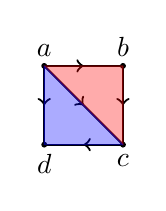
\begin{tikzpicture}[line join = round, line cap = round]
                \coordinate [label=above:$a$] (a) at (10,1);
                \coordinate [label=below:$d$] (d) at (10,0);
                \coordinate [label=above:$b$] (b) at (11,1);
                \coordinate [label=below:$c$] (c) at (11,0);

                \begin{scope}[decoration={markings,mark=at position 0.5 with {\arrow{to}}}]
                  \draw[fill] (a) circle [radius=0.03];
                  \draw[fill] (d) circle [radius=0.03];
                  \draw[fill] (b) circle [radius=0.03];
                  \draw[fill] (c) circle [radius=0.03];
                  % 6th
                  \draw[thick, postaction={decorate}] (a)--(b);
                  \draw[thick, postaction={decorate}] (a)--(d);
                  \draw[thick, postaction={decorate}] (b)--(c);
                  \draw[thick, postaction={decorate}] (c)--(d);
                  \draw[thick, postaction={decorate}] (a)--(c);
                \end{scope}
                \filldraw [opacity=.33,red] (10,1) -- (11,1) -- (11,0) -- cycle;
                \filldraw [opacity=.33,blue] (10,1) -- (10,0) -- (11,0) -- cycle;
              \end{tikzpicture}
              \end{center}
              
              The chain complex is $0 \rightarrow \mathbb{Z}^2 \xrightarrow{\partial_2} \mathbb{Z}^5 \xrightarrow{\partial_1} \mathbb{Z}^4 \rightarrow 0$. The matrices $M_2$ and $M_1$ of $\partial_2$ and $\partial_1$ without the indicated bases are:
              \begin{align*}
                M_2 = \begin{array}{c}\\ab\\bc\\cd\\ad\\ac\end{array}\left(\begin{array}{cc}abc&acd\\1&0\\1&0\\0&1\\0&-1\\-1&1\end{array}\right), M_1 = \begin{array}{c}\\d\\c\\b\\a\end{array}\left(\begin{array}{ccccc}ab&bc&cd&ad&ac\\0&0&1&1&0\\0&1&-1&0&1\\1&-1&0&0&0\\-1&0&0&-1&-1\end{array}\right)
              \end{align*}
              \\
              Then $\partial_1$ (ie $M_1$) induces a map of $\mathbb{Z}[t]$ - modules $\mathbb{Z}[t]^{\oplus5} \xrightarrow{M_1} \mathbb{Z}[t]^{\oplus4}$:
              \begin{align*}
                \underline{V} = \left(\begin{array}{c}p_1(t)\\p_2(t)\\p_3(t)\\p_4(t)\\p_5(t)\\\end{array}\right) \mapsto M_1 \underline{V}_\bullet
              \end{align*}
              \\
              Using the grading (filtration) on the simplicial complex we get a chain complex of graded $\mathbb{Z}[t]$ - modules\\
              $0 \rightarrow (t^4)\oplus(t^5) \xrightarrow{\partial_2^1} (t)^{\oplus2}\oplus(t^2)^{\oplus2}\oplus(t^3) \xrightarrow{\partial_1^1} (t)^{\oplus2}\oplus(1)^{\oplus2} \rightarrow 0$\\
              by the procedure defined on \cite{Zomorodian_Carlsson_2005}. The respective matrices are (without same bases)
              \begin{align*}
                M_2' = \begin{array}{c}\\ab\\bc\\cd\\ad\\ac\end{array}\left(\begin{array}{cc}abc&acd\\t^3&0\\t^3&0\\0&t^3\\0&-t^3\\-t^3&t^3\end{array}\right), M_1' = \begin{array}{c}\\d\\c\\b\\a\end{array}\left(\begin{array}{ccccc}ab&bc&cd&ad&ac\\0&0&t&t&0\\0&1&-t&0&t^2\\t&-t&0&0&0\\-t&0&0&-t^2&-t^2\end{array}\right)
              \end{align*}
              \\
              \underline{Note:} In Carlsson-Zomordian there is no difference in notation between $M_i$ and $M_i'$. Also, for the algorithm they order the elements such that the degree decreases down to rows. If we work in $\mathbb{R}[t]$, the matrices will be the same. In $\mathbb{Z}/2\mathbb{Z}[t]$ there won't be difference between $\pm 1$.\\
              
            \section{Computing Vietoris-Rips persistence barcodes using Ripser}

            In order to explicitly calculate persistence homology groups of point cloud data, I have created a Python scrip, that randomly generates points in a topological space, with and without noise, and then by
            using Ripser.py package, it calculates and plots Vietoris-Rips persistence barcodes. The library used is actually a wrapper around the original software written in C++. Before introducing details and results of my implementation, we will consider details in optimization, methodology, computation and implementation of the Ripser software.

            Ripser is a software design and implemented to calculate Vietoris-Rips persistence barcodes. The algorithm uses
            an implicit representation of the co-boundary operator and of the filtration order. Ripser has been optimized by
            avoiding any explicit construction and storage of the filtration co-boundary matrix, resulting in a significant improvement in time and memory usage.

            The predominant approach to persistence computation consist of two steps: the generation of a filtration
            boundary matrix, and the computation of persistence barcodes using matrix reduction. Often, the construction of the filtration boundary matrix becomes
                the bottleneck for the computation of Vietoris-Rips barcodes.

            That is why, Ripser takes a different approach by avoiding construction and storage of the whole filtration boundary matrix. The algorithm discards parts of the matrix and recomputes them when necessary. To reduce the memory usage, Ripser does not use an explicit matrix data structure, but uses a arithmetic operator,
            that recomputes the co-boundary map of a simplex whenever needed. The filtration is specified using another algorithmic operator for
            comparing simplices with respect to their appearance in the filtration order.

            The computation of persistent homology implemented in Ripser is based on matrix reduction and uses four key
            optimizations in order to achieve an efficient implementation:

            \begin{enumerate}
             \item Clearing birth columns:
             Avoid computation of unnecessary cycles, by using the spectral structure of a boundary matrix $D$, $D^2 = 0$
             \item Cohomology :
             Using Cohomology to compute persistence barcodes, since it is faster
             \item Implicit representation of boundary and reduced boundary matrices:
              Decouple the description of the filtration and of the boundary operator, representing the boundary matrix only algorithmically
                instead of explicitly, and to avoid the storage of the entire unreduced and reduced boundary matrices, retaining
                only the much smaller reduction matrix encoding the column operations
            \item Apparent and emergent pairs :
            The construction of the co-boundary matrix columns can be shortcut when a
            certain easily identified type of persistence pair, called an emergent co-face pair, is encountered
            \end{enumerate}

            To construct the algorithm, Ripser Software makes use of simplicial complexes and filtaration introduced in chapter \ref{chapter1}, with focus on the Vietoris Ripser complex, defined in \ref{rips}. Despite the Vietris -Rips filtration, a re-indexing and refinement of the filtration is used. In order to compute persistent homology, one needs to apply one further step of
            re-indexing, refining the essential filtration to an essential simplexwise one.

            To ease the computation of the Vietoris-Rips filtration, Ripser makes use of sub-level sets of functions and persistent homology. The Ripser package considers only simplicial homology with
            coefficients in prime field $\mathbb{F}_p$. The homology computation is made possible by using simplexwise refinement. A simplexwise filtration gives rise to a filtration boundary matrix,
            which is the matrix of the boundary operator of the chain complex $C_*(K)$ with respect to the ordered basis given by the oriented simplices in filtration order.

            During computation simplices are indexed in a combinatorial number system. Also, Ripser defines a refinement of the Vietoris-Rips filtration to an essential simplexwise filtration, as required for the computation of persistent homology. The simplexes are ordered by increasing diameter, then by increasing dimension and then by decreasing lexicographic vertex order. The result is called the
            \emph{lexicographically refined Vietoris-Rips filtration}.

            \subsection{Computation and Implementation}

            In the center of the algorithm for computing persistent homology, there is the matrix reduction method. The matrix reduction method is similar to the one introduced in the previous section. However, since the matrix reduction process can be expensive in time and memory usage, a technique for clearing columns is used.
            Another interesting approach is the choice to opt for computing persistence barcodes using co-homology instead of homology of Vietoris-Rips filtration. This approach is backed up by de Silva at all \cite{de_Silvia}, and it further optimizes the clearing of columns. Furthermore, as already mentioned before, the matrix reduction is done implicitly.
            Apart from the computation techniques mentioned above, there are several more optimizations that are
            presented in detail in \cite{Bauer_2019}

            In regards to the implementation, some important data structures of the C++ implementation of Ripser algorithm are:

            \begin{itemize}
             \item Input: The input for Ripser is a finite metric space $(X, d)$, encoded in a comma (or whitespace, or other nonnumerical character) separated list as either a distance matrix (full, lower, or upper triangular part), or as a list
of points in some Euclidean space
            \item Vertices and Simplices: Vertices are identified with natural numbers ${0, . . . , n ? 1}$, where n is the cardinality of
the input space. Simplices are indexed by natural numbers according to the combinatorial number system.
            \item Coefficients: Ripser supports the computation of persistent homology with coefficients in a prime field $\mathbb{F}_p$, for any prime number $p < 2^{16}$
            \item Column and matrix data structures: The basic data type for entries in a $(diameter_entry_t$) boundary or
coefficient matrix is a tuple consisting of a simplex index $(index_t)$, a floating point value $(value_t)$ caching
the diameter of the simplex with that index, and a coefficient $(coeff_t)$ if coefficients are enabled.

            \end{itemize}

            \subsection{Details and Results}

            The Python project is designed and implemented as a command line tool, that would allow the user to enter the name
            of a common space, the number of points, and the presence or absence of noise.

            The application can be supplied with 3 different options - ``space'', ``points'', and ''no\_noise``. The options ``space'' (--space or -s) stands for the different types of spaces that can be used. By default a sphere in $\RR^3$  shall be applied. Other options include a cylinder in $\RR^3$ (cylinder\_3), a torus in $\RR^3$ (torus\_3) and $\RR^4$ (torus\_4), klein bottle in $\RR^4$ (klein\_bottle\_4), projective plane in $\RR^4$ (pro\_plane\_4) and $\RR^6$ (pro\_plane\_6). After that, we have a ``points'' (--points or -p) parameter, indicating the number of points to be generated, where by default 500 shall be outputted. Last, the ``no\_noise'' (-n or --no-noise) parameter is whether or not to add noise to the generated points - it being enabled by default.

            The application uniformly generates the number of points inputted by the user into a square $1 \times 1$. Then the resulting points are saved in a $n$-dimensional array and used as a domain for the functions that are parameterizing surfaces that are included in the application. The points in the square are mapped on the surface of a common space. When the parameter "$-n$" is passed through the command line to the application, noise is introduced in the mapping of the points to the appropriate surface. The noise can generated randomly as uniform distribution or a Gaussian distribution, where the user can choose the $\sigma$ and standard deviation, or the bounds for the uniform segment.

            If the space is embedded in $\mathbb{R}^3$ the points generated on the surface will be plotted in a 3D graph. Regardless the generated points will be outputted on the console. Then the application will pop out a figure of the calculation of Vietoris-Rips persistence barcodes up to the homology specified in the code. Each persistent diagram is a pair (birth time, death time). After that another figure will pop up showing separately the computations of the Vietoris-Rips persistence barcodes in the respective homology. The last graph plots life time of each point instead of birth and death.


            \textbf{Sphere in $\mathbb{R}^3$}.\\
              Command: \textit{python generator.py --space sphere\_3 -points 500}

              \begin{figure}[H]
                \centering
                \begin{subfigure}[b]{0.45\linewidth}
                  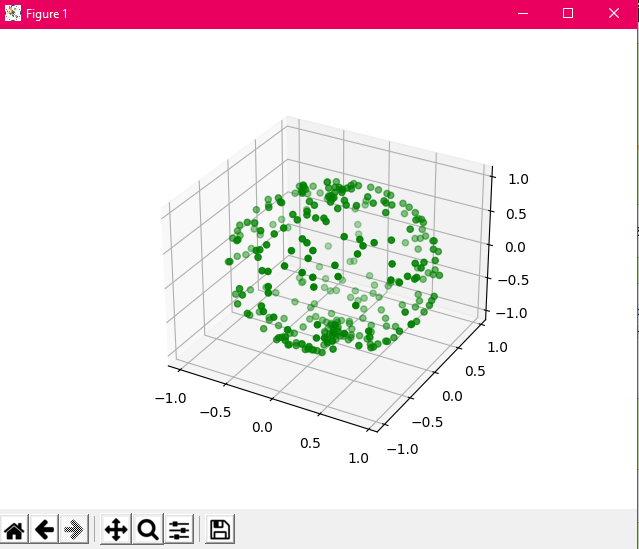
\includegraphics[width=\linewidth]{./ripser/on_sphere.PNG}
                  \caption{Plot.}
                \end{subfigure}
                \begin{subfigure}[b]{0.45\linewidth}
                  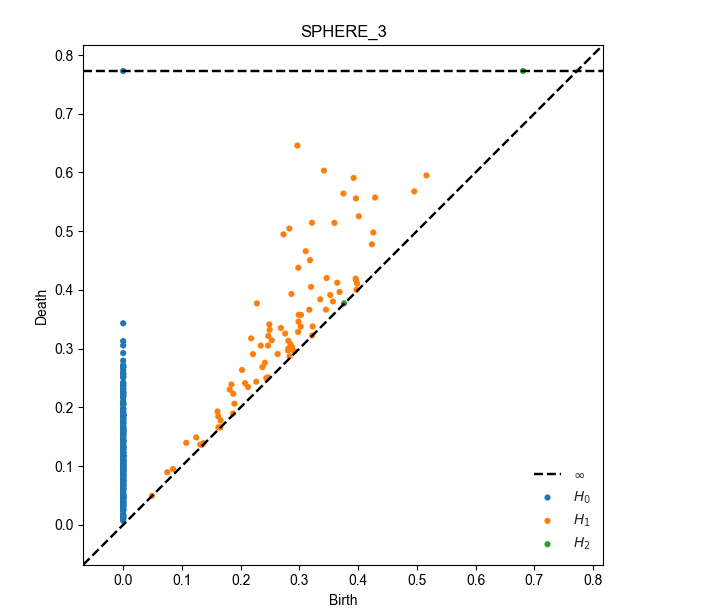
\includegraphics[width=\linewidth]{./ripser/on_sphere_homology.PNG}
                  \caption{Death birth all together.}
                \end{subfigure}
                \caption{Plot and Death birth graphs.}
                \label{fig: plot death}
              \end{figure}

              \begin{figure}[H]
                \centering
                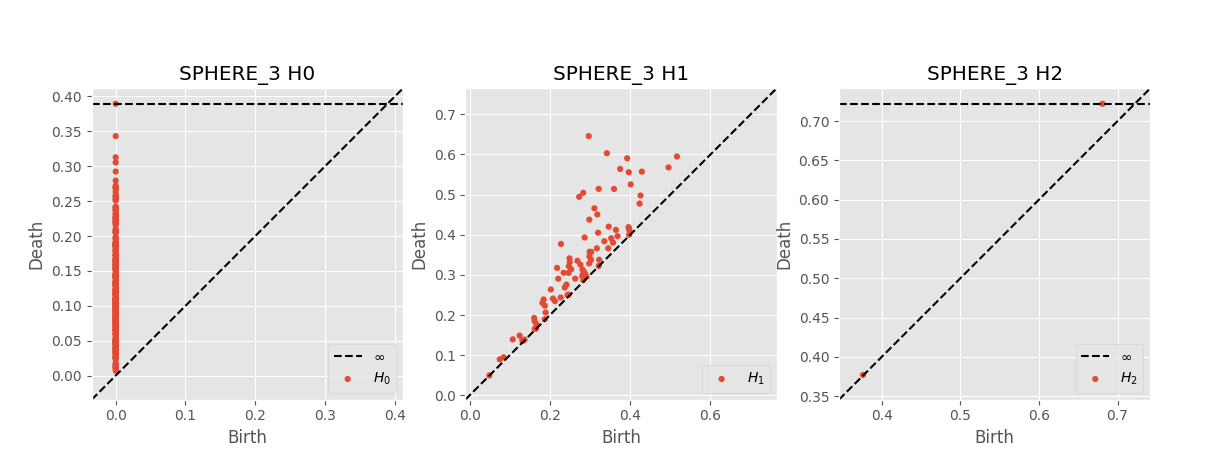
\includegraphics[width=\linewidth]{./ripser/on_sphere_sep_homology.PNG}
                \caption{Separate homology.}
                \label{fig:sep hom}
              \end{figure}

              \begin{figure}[H]
                \centering
                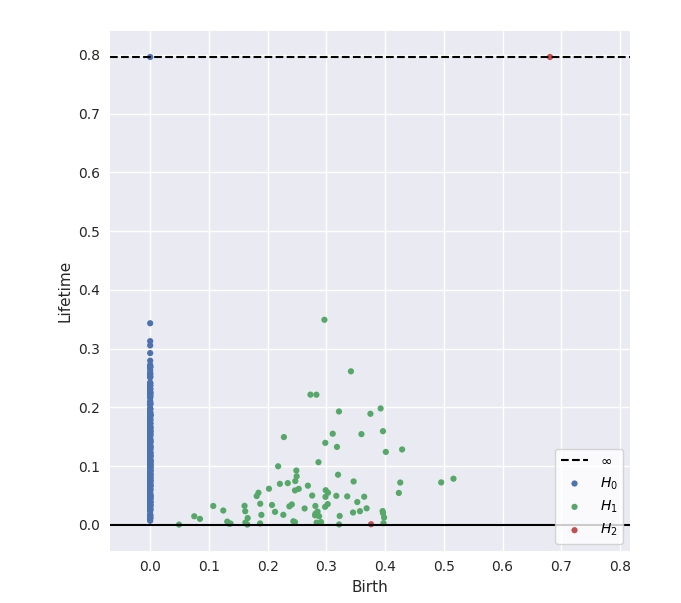
\includegraphics[width=0.5\linewidth, scale=0.5]{./ripser/on_sphere_lifetime.PNG}
                \caption{Lifetime persistent diagram.}
                \label{fig:sep hom}
              \end{figure}

              \textbf{Cylinder in $\mathbb{R}^3$}.\\
              Command: \textit{python generator.py --space cylinder\_3 -points 500}

              \begin{figure}[H]
                \centering
                \begin{subfigure}[b]{0.45\linewidth}
                  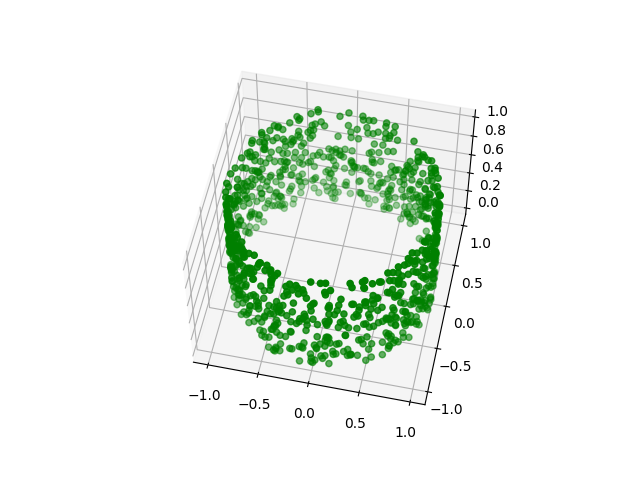
\includegraphics[width=\linewidth]{./ripser/on_cylinder.png}
                  \caption{Plot.}
                \end{subfigure}
                \begin{subfigure}[b]{0.45\linewidth}
                  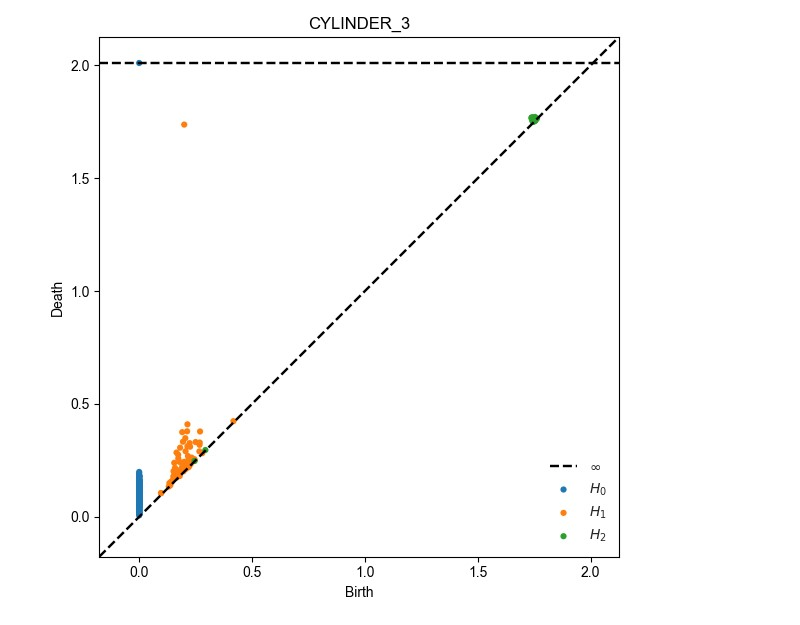
\includegraphics[width=\linewidth]{./ripser/on_cylinder_pers_homology.jpg}
                  \caption{Death birth all together.}
                \end{subfigure}
                \caption{Plot and Death birth graphs.}
                \label{fig: plot death}
              \end{figure}

              \begin{figure}[H]
                \centering
                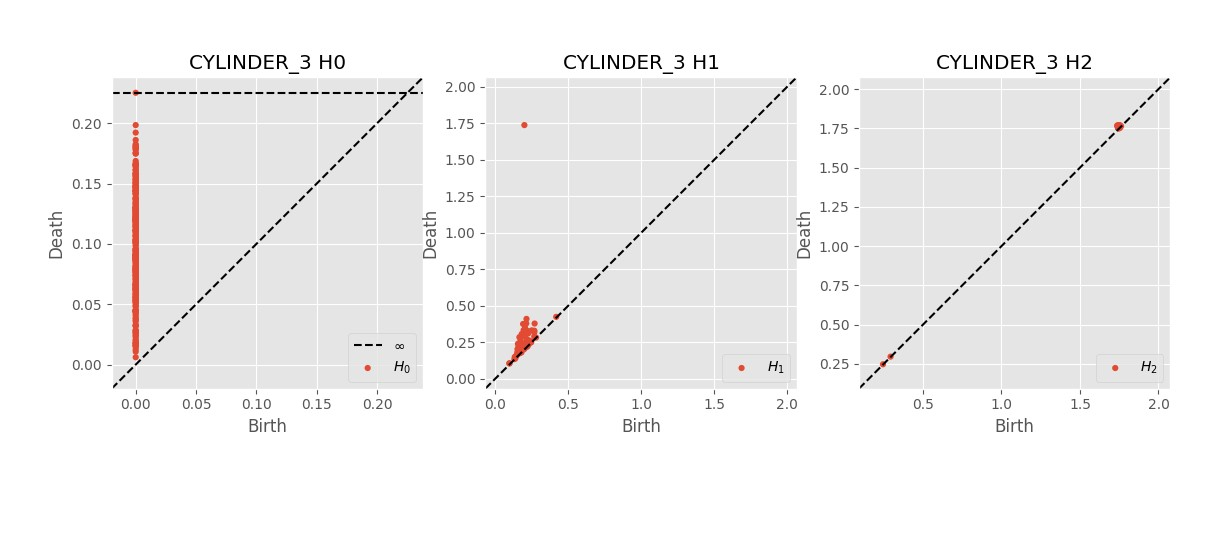
\includegraphics[width=\linewidth]{./ripser/on_cylinder_pers_homology_sep.jpg}
                \caption{Separate homology.}
                \label{fig:sep hom}
              \end{figure}

              \begin{figure}[H]
                \centering
                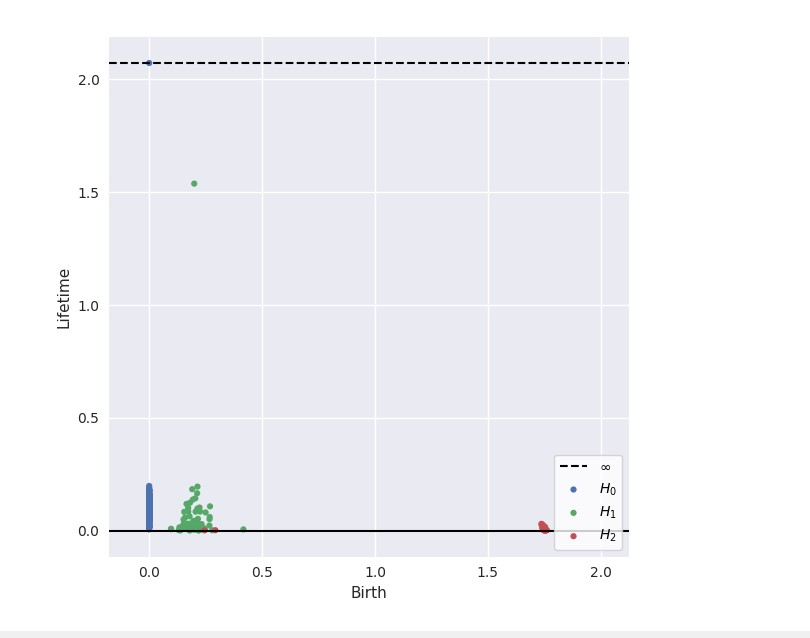
\includegraphics[width=0.5\linewidth, scale=0.5]{./ripser/on_cylinder_lifetime.jpg}
                \caption{Lifetime persistent diagram.}
                \label{fig:sep hom}
              \end{figure}

              \textbf{Random Sphere in $\mathbb{R}^3$}.\\
              Command: \textit{python generator.py --space sphere\_3 -points 500 -n}

              \begin{figure}[H]
                \centering
                \begin{subfigure}[b]{0.45\linewidth}
                  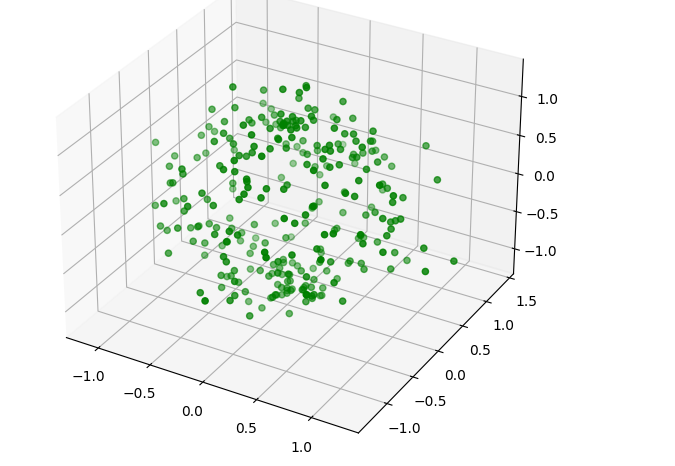
\includegraphics[width=\linewidth]{./ripser/rand_sphere.PNG}
                  \caption{Plot.}
                \end{subfigure}
                \begin{subfigure}[b]{0.45\linewidth}
                  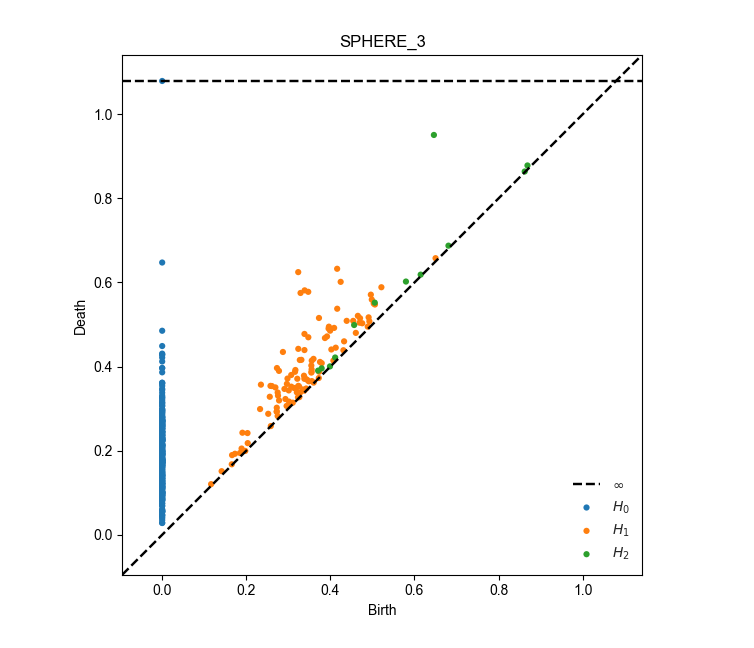
\includegraphics[width=\linewidth]{./ripser/rand_sphere_homology.PNG}
                  \caption{Death birth all together.}
                \end{subfigure}
                \caption{Plot and Death birth graphs.}
                \label{fig: plot death}
              \end{figure}

              \begin{figure}[H]
                \centering
                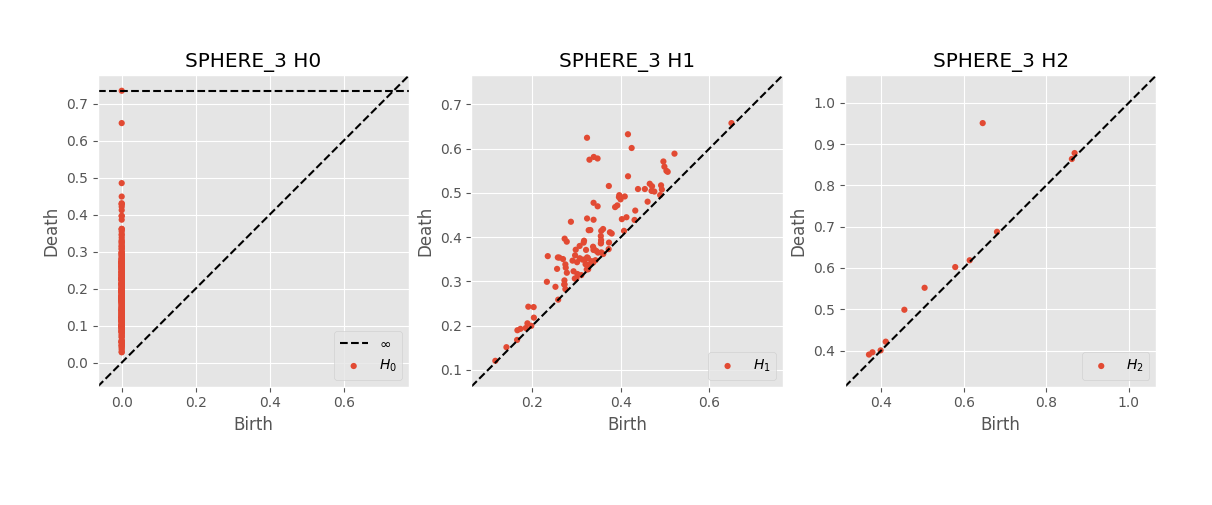
\includegraphics[width=\linewidth]{./ripser/rand_sphere_homology_seperate.PNG}
                \caption{Separate homology.}
                \label{fig:sep hom}
              \end{figure}

              \begin{figure}[H]
                \centering
                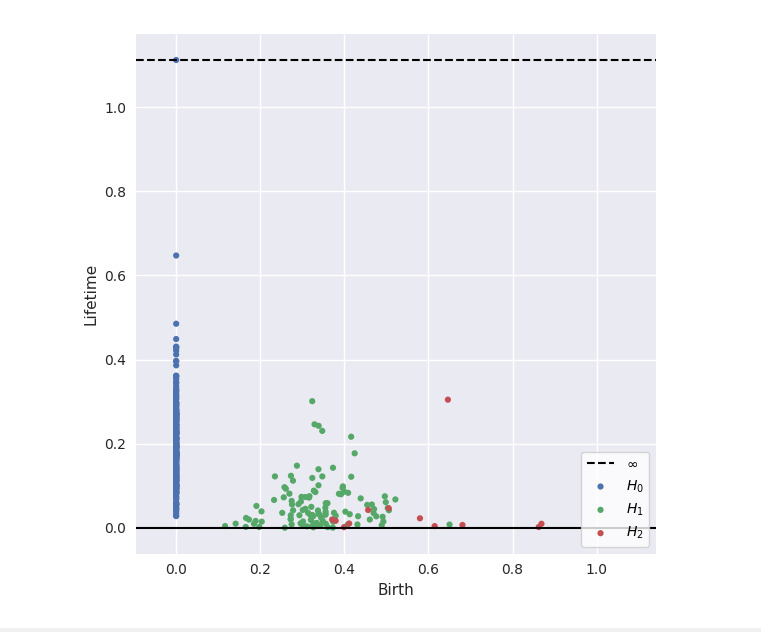
\includegraphics[width=0.5\linewidth, scale=0.5]{./ripser/rand_sphere_lifetime.PNG}
                \caption{Lifetime persistent diagram.}
                \label{fig:sep hom}
              \end{figure}

              \textbf{Random Cylinder in $\mathbb{R}^3$}.\\
              Command: \textit{python generator.py --space cylinder\_3 -points 500 -n}

              \begin{figure}[H]
                \centering
                \begin{subfigure}[b]{0.45\linewidth}
                  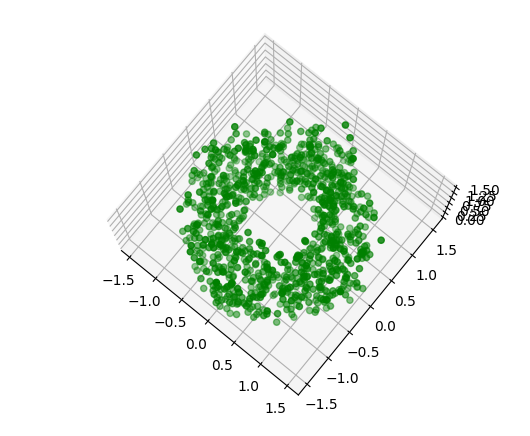
\includegraphics[width=\linewidth]{./ripser/rand_cyl.PNG}
                  \caption{Plot.}
                \end{subfigure}
                \begin{subfigure}[b]{0.45\linewidth}
                  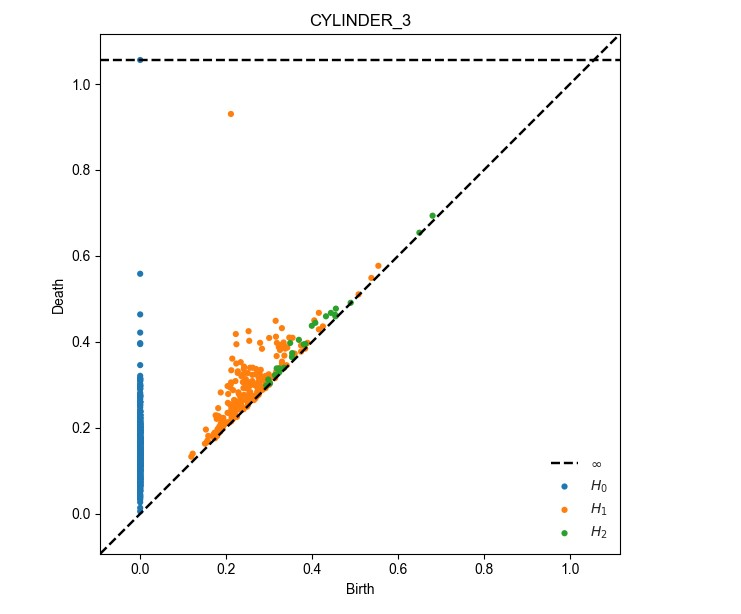
\includegraphics[width=\linewidth]{./ripser/rand_cyclinder_per_homology.jpg}
                  \caption{Death birth all together.}
                \end{subfigure}
                \caption{Plot and Death birth graphs.}
                \label{fig: plot death}
              \end{figure}

              \begin{figure}[H]
                \centering
                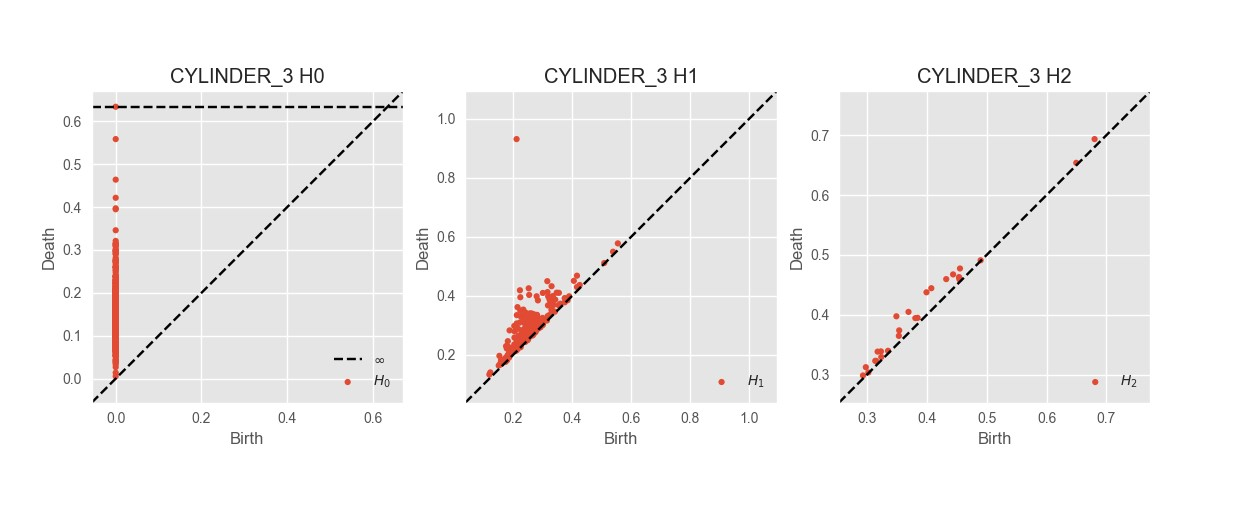
\includegraphics[width=\linewidth]{./ripser/rand_cyclinder_per_homology_seperate.jpg}
                \caption{Separate homology.}
                \label{fig:sep hom}
              \end{figure}

              \begin{figure}[H]
                \centering
                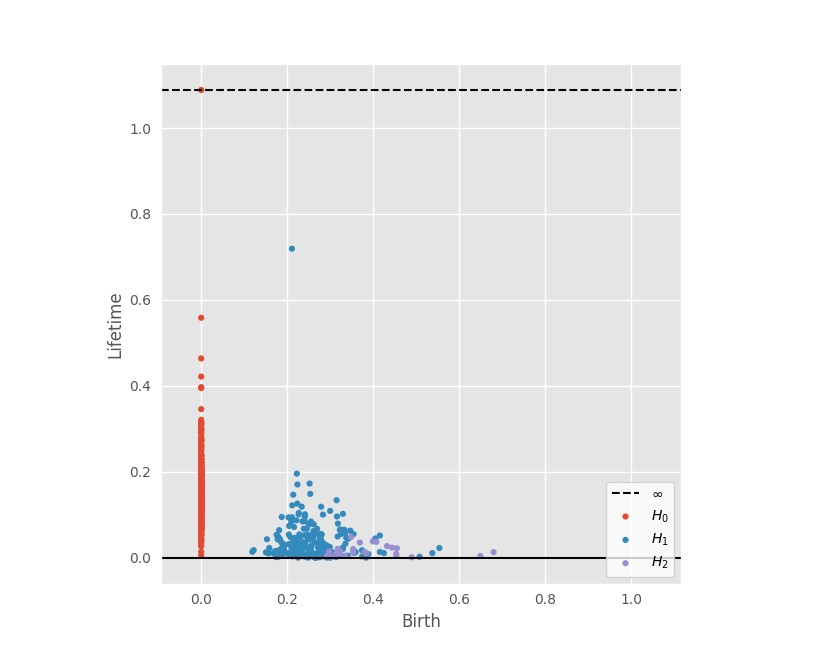
\includegraphics[width=0.5\linewidth, scale=0.5]{./ripser/rand_cylinder_lifetime.jpg}
                \caption{Lifetime persistent diagram.}
                \label{fig:sep hom}
              \end{figure}





\bibliographystyle{alpha}
\bibliography{biblio}



\end{document}
